\documentclass{scrreprt}

\usepackage[utf8]{inputenc}
\usepackage[ngerman]{babel}
\usepackage{amsmath}
\usepackage{amsthm}
\usepackage{amssymb}
\usepackage{mathtools}
\usepackage{graphicx}


\newtheorem{defi}{Definition}
\newtheorem{satz}{Satz}

\allowdisplaybreaks
\parskip 12pt

\begin{document}


\thispagestyle{empty}

\begin{center}

    %\rule{0mm}{3cm}

    \vspace{3cm}

    
\includegraphics[width=.8\textwidth]{uos.png}

    \vspace{1cm}

    {\huge\textbf{Synchrone Flow-Shop-Probleme mit Ressourcen und Rüstkosten}}

    \vspace{2ex}

    \vspace{1cm}



    \vspace{2ex}

    {\Large\textsc{Sebastian Brockmeyer}}

    \vspace{3cm}

    {\Large\textsc{M A S T E R A R B E I T}}

    \vspace{2cm}

    {\Large{September 2014}}

    \vspace{1cm}

    {Gutachter:}

    \vspace{2ex}

    {\Large{Prof. Dr. Sigrid Knust \\ Dipl.-Math. Stefan Waldherr}}

\end{center}

\chapter*{Vorwort}
Ich möchte in erster Linie meinen beiden Betreuern und Gutachtern, Prof. Dr. Sigrid Knust und Stefan Waldherr,
für ihre außerordentlich umfangreiche Unterstützung beim Erstellen dieser Arbeit danken.
Es ist nicht leicht, sich vorzustellen, wie die Betreuung einer Abschlussarbeit noch besser ablaufen kann.
Darüber hinaus möchte ich meiner Freundin ganz herzlich dafür danken,
dass sie vor allem in den letzten Tagen des Schreibens einen Großteil der häuslichen Pflichten auf sich genommen hat,
um mir ein relativ ungestörtes Arbeiten zu ermöglichen.
Diese Leistung gehört noch mehr gewürdigt, wenn man bedenkt, dass in dieser Zeit ein Umzug vorbereitet werden musste
und sie fast den gesamten Hausrat allein in Umzugskartons verstaut hat.

\chapter*{Kurzfassung}
Bei synchronen Flow-Shop-Problemen handelt es sich um Produktions\-planungs\-probleme, 
bei denen die Jobs immer nur synchron zur nächsten Maschine gelangen können.
D.h. ein Job kann erst dann zur nachfolgenden Maschine gelangen, wenn nicht nur diese, 
sondern auch alle anderen Maschinen mit ihrem jeweiligen Arbeitsschritt abgeschlossen haben.
Ziel ist es, die Jobs so anzuordnen, dass die gesamte Bearbeitungszeit minimiert wird.
Dazu werden einige Heuristiken entwickelt und mit bestehenden Verfahren verglichen.

Zusätzlich können die Jobs Ressourcen benötigen, die nur in begrenzter Menge vorhanden sind, aber wieder freigegeben werden, 
wenn der jeweilige Job die letzte Maschine passiert hat. 
Es kostet zusätzliche Zeit (Rüstkosten), wenn eine Ressource nach der Fertigstellung eines Jobs ausgetauscht werden muss.
In dieser Masterarbeit wird das Problem mit zwei Dekompositionsansätzen in mehreren Schritten gelöst. 
Dabei wird ein Spezialfall des Problems, der bei einem Küchenhersteller auftritt, besonders intensiv behandelt. 
Es werden sowohl exakte als auch heuristische Verfahren entwickelt und anschließend evaluiert.

\chapter*{Abstract}
Synchronous flow shop problems are production planning problems,
where the jobs can only get synchronously to the next machine.
I.e. a job cannot get to the following machine until then all machines, not only that one,
have completed their jobs.
The goal is to arrange the jobs in such a way that the makespan is minimized.
On that point, several heuristics are developed and compared to existing procedures.

Additionally, the jobs might need resources with only limited amounts at disposal, but they are reusable 
as soon as the respective job passed the last machine.
It takes additional setup time whenever a resource has to be exchanged after a job's completion.
In this master thesis the problem is solved in several steps with two decomposition approches.
A special case of this problem arising at a kitchen manufacturer is discussed in particular.
Both, exact and heuristic procedures are developed and, finally, discussed.


\tableofcontents


\chapter{Einleitung}
Bei synchronen Flow-Shop-Problemen handelt es sich um Produktions\-planungs\-probleme,
bei denen die Jobs sich immer nur synchron zur nächsten Maschine bewegen können.
Im Gegensatz zum klassischen (asynchronen) Flow-Shop, bei dem die Jobs immer sofort nach Fertigstellung an einer Maschine zur nächsten gelangen können,
müssen die Jobs beim synchronen Flow-Shop so lange warten, bis auch alle anderen Maschinen mit der Bearbeitung ihres jeweiligen Jobs fertig sind.
Die Komplexität synchroner Flow-Shop-Probleme wurde zuerst von Karabati und Sayin \cite{karabati} diskutiert.
Soylu et al. \cite{soylu} stellten einen Branch-and-Bound-Algorithmus vor, der die gesamte Fertigstellungsdauer minimiert, und liefern einen (fehlerhaften) Beweis, 
dass dieses Problem mit drei Maschinen $\mathcal{NP}$-schwer ist.
Waldherr und Knust korrigieren diesen Beweis in einem bis zum Zeitpunkt dieser Masterarbeit noch nicht veröffentlichten Paper \cite{preprint}.
Darüber hinaus betrachten sie einige Spezialfälle des synchronen Flow-Shops mit einer geringen Anzahl an dominierenden Maschinen.
Dominierende Maschinen zeichnen sich dadurch aus, dass ihre Prozesszeiten für alle Jobs mindestens so groß sind wie bei den übrigen Maschinen.

Das Konzept der dominierenden Maschinen aus der Arbeit von Waldherr und Knust basiert auf einer konkreten praktischen Anwendung von synchronen Flow-Shop-Pro\-ble\-men.
Es handelt sich dabei um einen in Bad Essen ansässigen Küchenhersteller.
In einer Fallstudie \cite{casestudy} haben Waldherr und Knust das bei diesem Küchenhersteller gegebene Optimierungsproblem genauer untersucht.
Es handelt sich dabei um einen synchronen Flow-Shop, wobei die zu produzierenden Jobs Ressourcen benötigen und die Produktionsanlage beim Einlegen eines Jobs
ggf. umgerüstet werden muss, was Rüstkosten verursacht.
U.a. durch dieses Praxisbeispiel ist auch diese Masterarbeit motiviert.

\section{Problembeschreibung}
\label{sec:Problembeschreibung}
Die Produktionsanlage be\-steht aus $m$ Stationen, in die die Jobs eingelegt werden.
Die Anlage bewegt die Stationen und die in ihnen befindlichen Jobs der Reihenfolge nach zu den Maschinen $M_1,\ldots,M_m$,
die außen, um die Anlage herum, aufgestellt sind und die einzelnen Produktionsschritte durchführen.
Dabei handelt es sich bei Maschine $M_1$ um das Einlegen des Jobs in die Anlage und nach der letzten Maschine $M_m$ wird das fertige Produkt entnommen.
Die Stationen stehen derart miteinander in Verbindung, dass sie sich immer nur gemeinsam fortbewegen können.
Die Anlage kann beispielsweise kreisförmig aufgebaut sein, wie in Abbildung \ref{abb:Anlage} dargestellt.
Aus diesem Grund wird die Fortbewegung der Stationen mit den Jobs zur jeweils nächsten Maschine als \textit{Rotation} bezeichnet,
auch wenn die Anlage nicht zwangsweise zyklische Gestalt haben muss.
\begin{figure}[h]
    \begin{center}
        \begin{tabular}{cc}
            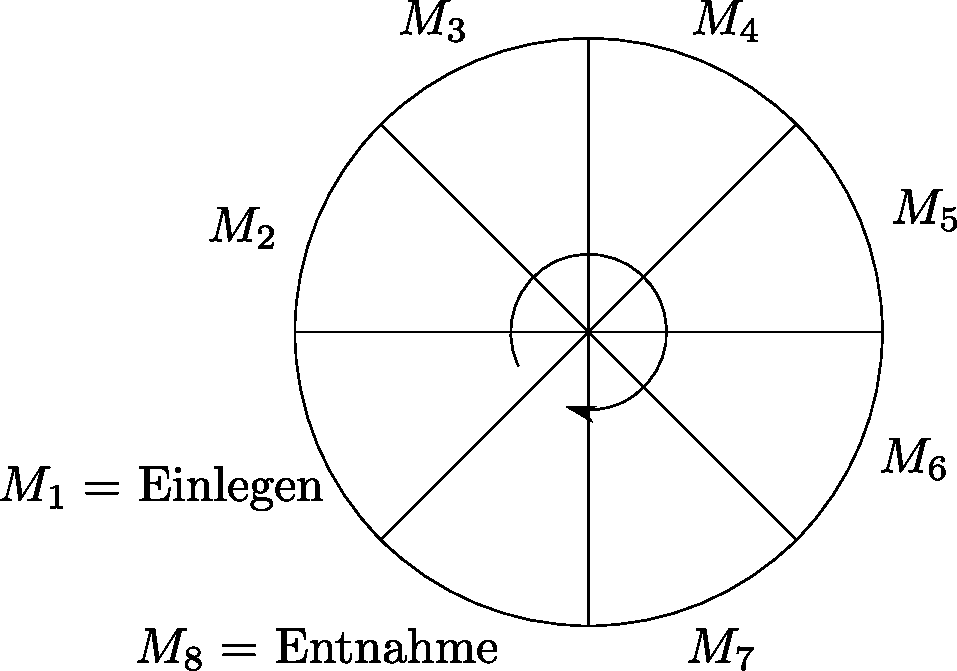
\includegraphics[width=.45\textwidth]{graphics/anlage.pdf}
            & 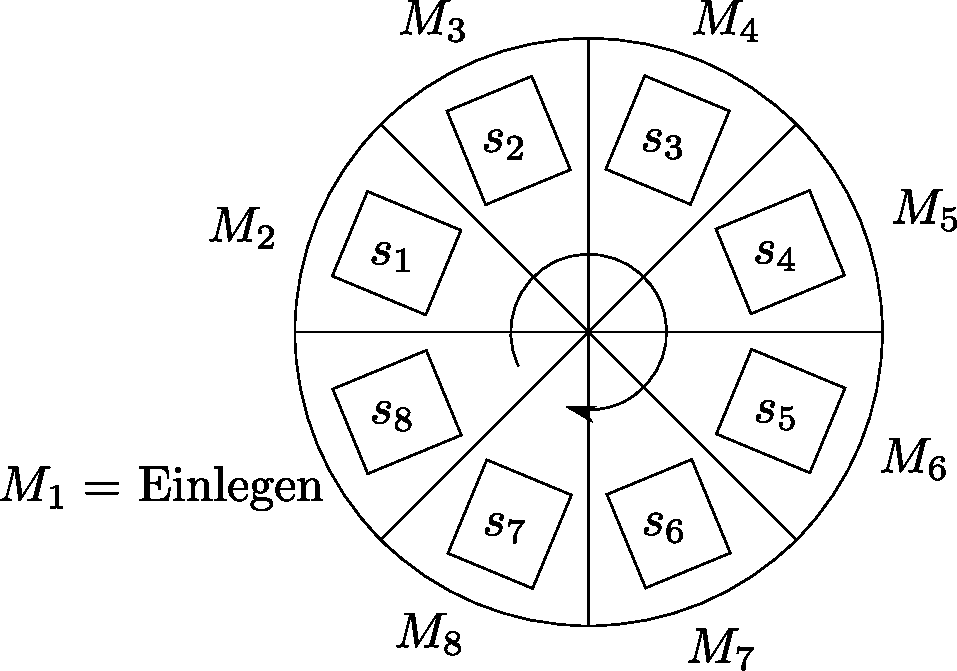
\includegraphics[width=.45\textwidth]{graphics/anlage2.pdf}
        \end{tabular}
    \end{center}
    \caption{
        \label{abb:Anlage}
        Kreisförmige Anlage mit $m=8$ Maschinen und Stationen, rechts nach einer Rotation. 
        Die Stationen, in die die Jobs eingelegt werden, drehen sich mit der Anlage zu den außen herum aufgestellten Maschinen.
    }
\end{figure}
Eine Rotation darf immer nur dann stattfinden, wenn alle Maschinen ihren Produktionsschritt an ihrem aktuellen Job
durchgeführt haben. Auf diese Weise können die Jobs, im Gegensatz zum klassischen (asynchronen) Flow-Shop, 
immer nur \textit{synchron} zur nachfolgenden Maschine gelangen.
Die Zeit, die zwischen zwei Rotationen vergeht, wird als \textit{Zykluszeit} bezeichnet.

Die zu produzierenden Jobs sind gegeben durch die Menge $N=\{1,\ldots,n\}$ 
und die Prozesszeiten von Job $j$ auf Maschine $M_i$ sind durch $p_{ij}$ gegeben.
Ein Plan für eine Beispielinstanz mit $n=5$ und $m=3$ ist in Abbildung \ref{abb:Bsp} zu sehen.
\begin{figure}[h]
    \begin{center}
        \begin{tabular}{c|ccccc}
                  & 1 & 2 & 3 & 4 & 5 \\ \hline
            $M_1$ & 4 & 1 & 2 & 5 & 4 \\ 
            $M_2$ & 6 & 5 & 5 & 2 & 5 \\
            $M_3$ & 5 & 6 & 4 & 4 & 4 
        \end{tabular}
    \end{center}
    \caption{
        \label{abb:Bsp}
        Beispielinstanz mit 5 Jobs und 3 Maschinen. Die Werte in der Tabelle sind die Prozesszeiten $p_{ij}$.
    }
\end{figure}
\begin{figure}
    \begin{center}
        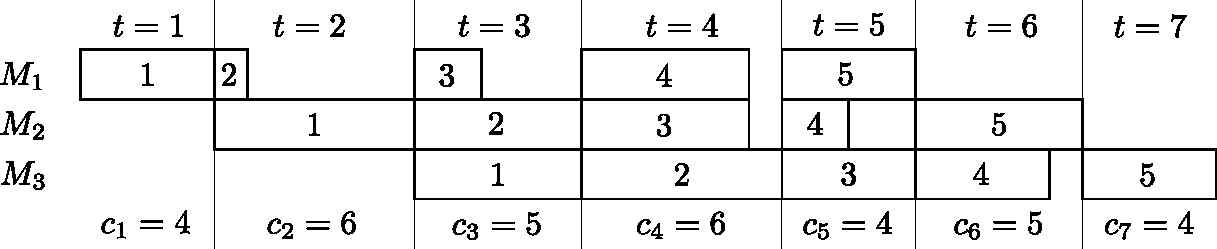
\includegraphics[width=.8\textwidth]{graphics/bspinit.pdf}
    \end{center}
    \begin{center}
        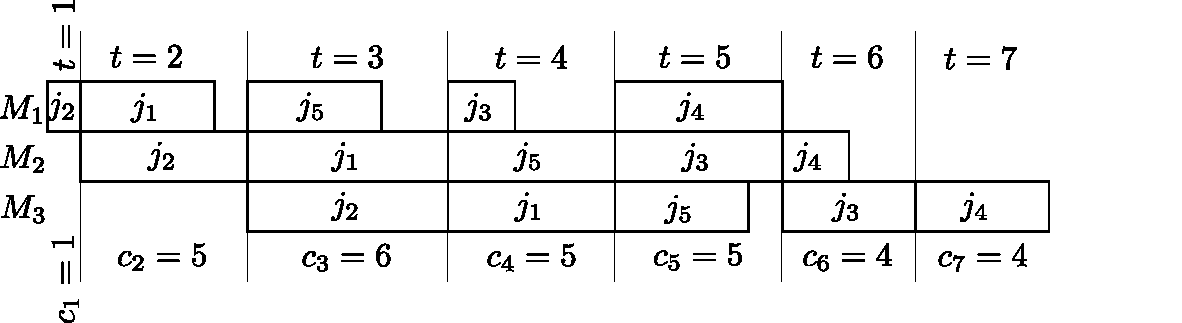
\includegraphics[width=.8\textwidth]{graphics/bspopt.pdf}
    \end{center}
    \caption{
        \label{abb:gantt}
        Gantt-Diagramme der initialen Reihenfolge der Beispielinstanz in Abb. \ref{abb:Bsp} mit $C_{\max}=34$
        und einer optimalen Reihenfolge mit $C_{\max}=30$.
    }
\end{figure}
Ziel ist es, eine Permutation $\pi$ der Jobs zu erstellen, die die gesamte Produktionsdauer minimiert.
Diese Zielfunktion wird mit $C_{\max}$ bezeichnet.
Die Beispielinstanz, deren Plan in Abbildung \ref{abb:Bsp} zu sehen ist, ist in Abbildung \ref{abb:gantt} als Gantt-Diagramm aufgetragen.
Oben sind die Jobs in der initialen Reihenfolge (1-2-3-4-5) und unten in einer bezüglich $C_{\max}$ optimalen Reihenfolge (2-1-5-3-4).
Die Zykluszeiten $c_t$ mit $1\leq t\leq n+m-1$ berechnen sich wie folgt:
\[ c_t = \max_{i=\max\{1,t-n+1\}}^{\min\{t,m\}} p_{i\pi_{t-i+1}} \]
Die Zielfunktion lässt sich also durch $C_{\max} = \sum_{t=1}^{n+m-1} c_t$ berechnen.
Andere Zielfunktionen werden in dieser Masterarbeit nicht betrachtet.

Eine Teilmenge $D \subseteq \{1,\ldots,m\}$ der Maschinen heißt \textit{dominierend}, wenn 
\[ p_{dj} \geq p_{ej} \quad \forall j\in N, d\in D, e\not\in D \] 
ist. 
Die Prozesszeiten aller Jobs auf dominierenden Maschinen sind also immer mindestens so groß wie die Prozesszeiten auf den restlichen Maschinen.
Treten dominierende Maschinen auf, müssen für die Berechnung der Zykluszeiten die Prozesszeiten auf den übrigen Maschinen also nicht betrachtet werden.
Dominierende Maschinen treten in der Praxis häufig auf. 
Bei dem Küchenhersteller aus Bad Essen sind z.B. zwei von acht Maschinen dominierend.
Diese beiden Maschinen sind dort außerdem benachbart, weshalb dieser Fall in dieser Masterarbeit besonders intensiv behandelt wird. 

Zusätzlich benötigen die Jobs unter Umständen Ressourcen (z.B. Paletten oder Klebeformen) aus einer Menge $R$, 
um in die Stationen eingelegt werden zu können. Diese Ressourcen können erst nach
Fertigstellung eines Jobs, also nachdem er nach Maschine $M_m$ aus der Anlage genommen wurde, wiederverwendet werden.
Sie sind allerdings nur in begrenzter Zahl vorhanden und im Allgemeinen ist nicht jede Ressource für jeden Job geeignet.
Für $j\in N$ sei $\rho_j\subseteq R$ die Menge der Ressourcen, die für $j$ geeignet ist.
Umgekehrt sei für $r\in R$ mit $\iota_r\subseteq N$ die Menge der Jobs bezeichnet, für die $r$ geeignet ist.
Wenn eine Station nach der Entnahme eines Jobs nach Maschine $M_m$ wieder an Maschine $M_1$ angelangt, kann es daher notwendig sein, 
vor dem Einlegen des nächsten Jobs die Ressource zu wechseln, 
wenn auf der Station zuvor Job $j\in N$ mit Ressource $r\in\rho_j$ fertiggestellt wurde 
und nun Job $j'\not\in\iota_r$ eingelegt werden soll.

Für die Ressourcen können folgende Situationen auftreten:
\begin{enumerate}
    \item Alle Ressourcen sind für alle Jobs geeignet, also $\rho_j=R$ für alle $j\in N$.
    \item Die Jobs lassen sich in disjunkte Gruppen unterteilen, so dass für alle Jobs aus einer Gruppe dieselbe Ressourcenmenge geeignet ist.
        Wenn also $\rho_i \cap \rho_j \neq \emptyset$, dann folgt $\rho_i=\rho_j$.
    \item Die Ressourcenmengen bilden Hierarchien. 
        D.h., wenn $\iota_q \cap \iota_r \neq \emptyset$, dann folgt $\iota_q \subseteq \iota_r$ oder $\iota_r \subseteq \iota_q$.
    \item Die $\rho_j$ sind beliebige Teilmengen von $R$.
\end{enumerate}%
Der erste Fall ist trivial, da niemals eine Ressource gewechselt werden muss.
Dies entspricht der Situation ohne Ressourcen und Rüstkosten.
In dieser Masterarbeit liegt der Fokus auf dem zweiten Fall.
Er ist dadurch motiviert, dass es in realen Anwendungsfällen häufig nicht der Fall ist, dass bei $n$ zu produzierenden Jobs alle $n$ Jobs unterschiedlich sind,
d.h. unterschiedliche Prozesszeiten und Ressourcen haben.
Stattdessen bietet ein Produzent eine gewisse Anzahl unterschiedlicher Güter an und ein Käufer gibt mehrere identische Güter auf einmal in Auftrag.
Diese identischen Jobs können dann als \textit{Jobgruppen} bezeichnet werden, für die es eine Menge an nur für sie geeigneten Ressourcen gibt.
Der dritte Fall ist vom Prinzip her vergleichbar mit einem Generalschlüssel, der in mehrere Schlüssellöcher passt,
wobei es für einzelne Schlüssellöcher auch speziell nur dafür passende Schlüssel gibt, die in die anderen Schlüssellöcher nicht passen.
Ressourcen können in ähnlicher Weise durch geringe Unterschiede für viele Jobs auf einmal oder nur für einzelne geeignet sein.
Der vierte Fall ist der allgemeinste und deckt alle anderen mit ab.
Er wird in dieser Arbeit nur kurz betrachtet (vgl. Abschnitt \ref{subsubsec:ZulaessigkeitBeiBeliebigenRessourcenteilmengen}).

Neben dem Wechsel von Ressourcen, der zusätzliche Zeit in Anspruch nimmt, können auch andere Formen von \textit{Rüstkosten}
auftreten. Z.B. kann es sein, dass an einer Station zunächst einige Umstellungen vorgenommen werden müssen, bevor der
neue Job eingelegt werden kann. Die Jobs können in Familien $\mathcal{F}$ eingeteilt werden, so dass beim Übergang
zwischen zwei Jobs aus den Familien $f$ und $g$ die Rüstkosten $s_{fg}$ auftreten.
Diese Rüstkosten können 
\begin{itemize}
    \item sowohl vom Vorgänger als auch vom Nachfolger abhängig sein ($s_{fg}$), 
    \item nur vom Nachfolger abhängig sein ($s_{fg} = s_{g}$) oder
    \item konstant sein ($s_{fg} = s > 0$).
\end{itemize}%
Dabei wird $s_{ff} = 0$ angenommen für alle $f\in\mathcal{F}$, es treten also keine Rüstkosten innerhalb einer Familie auf.
Wenn Ressourcen notwendig sind, können die Familien über die Ressourcen definiert werden:
Wenn $\rho_i=\rho_j$, dann gehören $i$ und $j$ zur gleichen Familie.
%Das setzt allerdings voraus, dass für $i$ und $j$ auf jeden Fall die selbe Ressource verwendet wird, falls sie in $\pi$ im Abstand von $m$ vorkommen.

Wenn Rüstkosten auftreten, soll nicht mehr nur die Summe aller Zykluszeiten minimiert werden, sondern zusätzlich noch die Summe aller auftretenden Rüstkosten.
Die Zielfunktion $C_{\max}$ lässt sich dann als 
\[ \min\left(\sum_{t=1}^{n+m-1}c_t +\sum_{i=1}^{n-m}s_{i,i+m}\right) \] 
formulieren, wobei hier die Rüstkosten direkt mit den Jobs statt mit den Familien indiziert sind.

\begin{figure}
    \begin{center}
        \begin{tabular}{c|ccccc}
            & $1$ & $2$ & $3$ & $4$ & $5$ \\ \hline
            $1$ & 0 & 8 & 5 & 9 & 4\\
            $2$ & 6 & 0 & 6 & 8 & 8\\
            $3$ & 4 & 7 & 0 & 5 & 4\\
            $4$ & 5 & 7 & 8 & 0 & 9\\
            $5$ & 4 & 5 & 8 & 9 & 0
        \end{tabular}
    \end{center}
    \caption{
        \label{abb:BspRes}
        Rüstkosten für die Beispielinstanz aus Tabelle \ref{abb:Bsp}.
        Beispielsweise treten Rüstkosten von $6$ auf, wenn von Job $2$ auf Job $1$ gewechselt werden muss.
    }
\end{figure}
In Abbildung \ref{abb:BspRes} ist eine mögliche Rüstkostentabelle für das Beispiel aus Abbildung \ref{abb:Bsp} gegeben.
Die initiale Reihenfolge (1-2-3-4-5) und eine optimale (4-2-3-1-5) sind in Abbildung \ref{abb:ganttres} als Gantt-Diagramm dargestellt.
\begin{figure}
    \begin{center}
        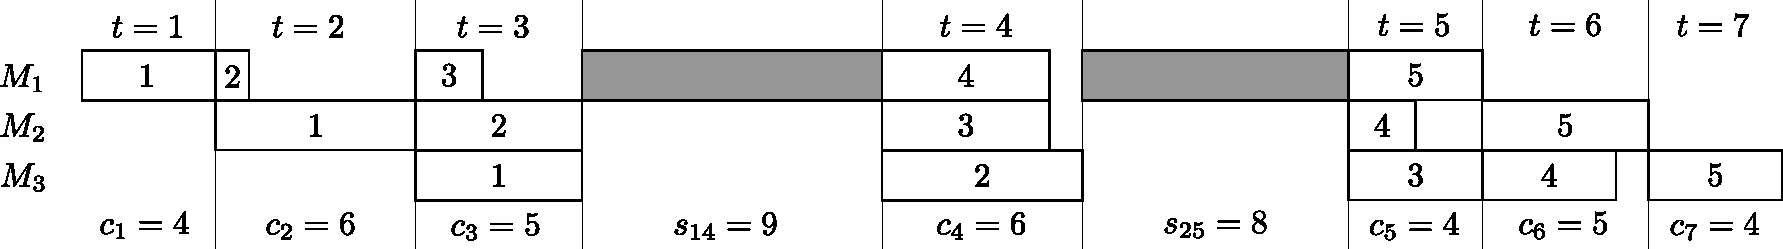
\includegraphics[width=\textwidth]{graphics/bspresinit.pdf}
    \end{center}
    \begin{center}
        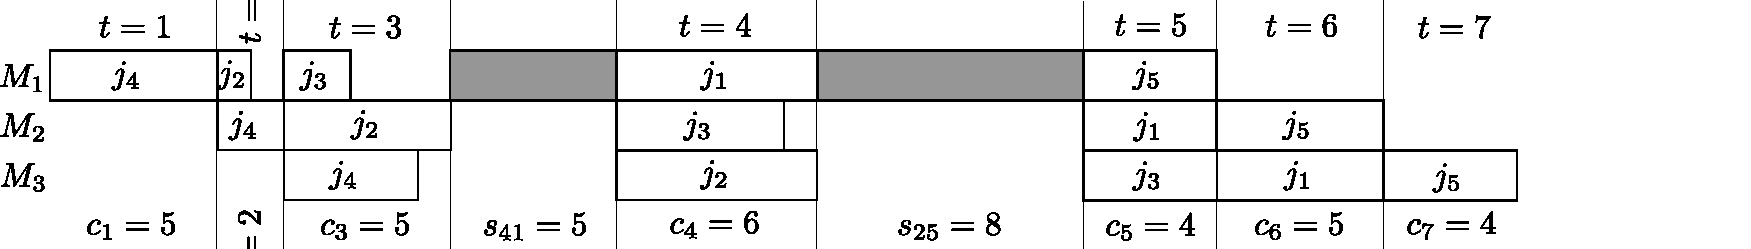
\includegraphics[width=\textwidth]{graphics/bspresopt.pdf}
    \end{center}
    \caption{
        \label{abb:ganttres}
        Initiale und eine optimale Lösung als Gantt-Diagramme für das Beispiel aus Abb. \ref{abb:Bsp} erweitert um Rüstkosten aus Abb. \ref{abb:BspRes}.
    }
\end{figure}

Insgesamt gilt es, neben der Reihenfolge $\pi$ auch ein Mapping $f:N\rightarrow R$ zu finden, 
das jedem Job $j\in N$ eine Ressource $r\in\rho_j$ zuweist und folgenden Ansprüchen genügt:
\begin{itemize}
    \item $f$ muss zulässig sein in dem Sinne, dass beim Einlegen jedes Jobs $j\in N$ eine Ressource $r\in\rho_j$ verfügbar ist
        (d.h., dass $r$ sich nicht gerade an anderer Stelle in der Anlage befindet).
    \item $f$ und $\pi$ zusammen sollen optimal sein in dem Sinne, dass die Summe aus den durch $\pi$ und $f$ definierten Zykluszeiten und 
        Rüstkosten minimal ist.
\end{itemize}

Im Folgenden wird ein Mixed Integer Linear Program (MIP) vorgestellt, dass das Gesamtproblem löst, allerdings ohne die Verfügbarkeit von Ressourcen zu beachten.
Dabei ist $N$ die Indexmenge der Jobs, also $N=\{1,\ldots,n\}$ und $T=\{1,\ldots,n+m-1\}$ ist die Indexmenge der Zykluszeiten.
Die Binärvariablen $x_{jk}$ geben für $j,k\in N$ an, an welcher Position $k$ in $\pi$
sich Job $j$ befindet. Es gilt $x_{jk}=1$ genau dann, wenn $j$ an Position $k$ ist ($\pi_k=j$). 
Die Binärvariablen $y_{jh}$ ($j,h\in N$) haben genau dann den Wert $1$, wenn Job $j$ genau $m$ Positionen vor Job $h$ in $\pi$ liegt ($\exists i:\pi_{i-m}=j \land \pi_i=h$).
Damit können in der Zielfunktion die Rüstkosten $s_{jh}$ aufsummiert werden, die beim Übergang von $j$ zu $h$ auftreten:
\begin{align}
    \text{min} \quad \sum_{t=1}^{n+m-1} &c_t + \sum_{j=1}^n \sum_{h=1}^n s_{jh} y_{jh} \label{allmip:obj}\\
    \text{s.t.}\quad \sum_{k=1}^n x_{jk} &= 1 & j\in N \label{allmip:1}\\
                     \sum_{j=1}^n x_{jk} &= 1 & k\in N \label{allmip:2}\\
    c_t &\geq \sum_{j=1}^n p_{t-k+1,j} \cdot x_{jk} & t\in T, k=\max\{1,t-m+1\},\ldots,\min\{n,t\} \label{allmip:3}\\
    y_{jh} + 1 &\geq x_{j,k-m} + x_{hk} & j,h\in N, k=m+1,\ldots,n \label{allmip:4}\\
    c_t &\geq 0 & t\in T \\
    x_{jk} &\in \{0,1\} & j,k\in N \\
    y_{jh} &\in \{0,1\} & j,h\in N
\end{align}
Die Nebenbedingungen (\ref{allmip:1}) und (\ref{allmip:2})
stellen sicher, dass sich jeder Job an genau einer Position in $\pi$ befindet und 
dass sich an jeder Position genau ein Job befindet.
In Nebenbedingung (\ref{allmip:3}) werden die Zykluszeiten bestimmt.
In (\ref{allmip:4}) werden die $y_{jh}$ auf $1$ gesetzt, wenn $x_{j,k-m}$ und $x_{hk}$ auf $1$ gesetzt sind.
In der Zielfunktion (\ref{allmip:obj}) wird die Summe aus allen
Zykluszeiten gebildet und die Summe aller auftretenden Rüstkosten $s_{jh}$.

Obwohl in diesem MIP nicht die Verfügbarkeiten von Ressourcen beachtet werden,
benötigt es schon bei $n=20$ mehrere Stunden zum Finden der optimalen Lösung.
Es ist also für Instanzen mit mehreren Tausend Jobs nicht geeignet.
Aufgrund dieser Tatsache ist eine heuristische Herangehensweise an 
synchrone Flow-Shop-Probleme mit Ressourcen und Rüstkosten eine gute Alternative.


\section{Motivation für Dekompositionsansätze}
In \cite{preprint} wird gezeigt, dass synchrone Flow-Shop-Probleme ohne Ressourcen und Rüstkosten $\mathcal{NP}$-schwer sind für $m>2$.
Versuche, dieses Problem -- oder auch einige Spezialfälle davon -- mit ganzzahliger linearer Programmierung optimal zu lösen, waren nur für sehr kleine Instanzen mit
$n<30$ in hinnehmbarer Zeit erfolgreich, was weit hinter praktischen Anforderungen zurückliegt (vgl. Abschnitt \ref{subsec:LineareProgrammierung}).
Aufgrund der Komplexität des Gesamtproblems (vgl. das MIP aus Abschnitt \ref{sec:Problembeschreibung}) sollen in dieser Arbeit zwei Dekompositionsansätze verfolgt werden,
die $C_{\max}$ in zwei Stufen getrennt nach Zykluszeiten und Rüstkosten optimieren:
\begin{enumerate}
    \item Zunächst wird eine Reihenfolge $\pi$ aufgestellt, ohne Ressourcen und Rüstkosten zu betrachten, so dass die Summe der Zykluszeiten möglichst gering ist.
        Anschließend wird ein zulässiges Mapping $f$ basierend auf $\pi$ erstellt, möglichst ohne nachträgliche Änderung an $\pi$ vorzunehmen,
        so dass die Summe der Rüstkosten minimiert wird.
    \item Es wird zuerst ein Mapping $f$ erstellt, so dass die Ressourcen zulässig zugewiesen sind und die durch die Ressourcenwechsel verursachten Rüstkosten minimal sind.
        Anschließend werden, ohne $f$ zu verändern, die Jobs so in einer Reihenfolge $\pi$ angeordnet, dass $C_{\max}$ möglichst minimal ist.
\end{enumerate}%
Beide Ansätze liefern natürlich im Allgemeinen keine optimalen Lösungen, da jeweils getrennt bezüglich $\pi$ und $f$ optimiert wird,
obwohl die optimale Lösung von beiden zusammen abhängig ist.
Außerdem sind selbst die aus den Ansätzen resultierenden Teilprobleme teilweise noch $\mathcal{NP}$-schwer.
Beispielsweise ist bei Ansatz (1) das Berechnen einer $C_{\max}$-optimalen Reihenfolge $\pi$ im Allgemeinen $\mathcal{NP}$-schwer. 
In dem Spezialfall, dass es nur eine dominierende Maschine gibt, ist es trivial, da $C_{\max}$ bei jeder Reihenfolge identisch ist.
Wenn es genau zwei benachbarte dominierende Maschinen gibt,
ist es mit dem Algorithmus von Gilmore und Gomory \cite{gg} in Polynomialzeit lösbar.
Bei der anschließenden Zuweisung von Ressourcen ist noch unbekannt, ob ein polynomieller Algorithmus existiert.
%Dies herauszufinden ist eines der Ziele dieser Arbeit.

Je nachdem, ob die Rüstkosten die Zykluszeiten dominieren oder umgekehrt, ist Ansatz (2) bzw. Ansatz (1) vielversprechender.


\chapter{Der erste Dekompositionsansatz}
\label{chap:DerErsteDekompositionsansatz}
Beim ersten Dekompositionsansatz wird zunächst eine (möglichst gute) Jobreihenfolge $\pi$ bestimmt.
Dabei werden Ressourcen und Rüstkosten außer Acht gelassen. 
Es wird also zunächst ausschließlich die Summe der Zykluszeiten optimiert. Anschließend wird ein Mapping $f$ aufgestellt,
so dass Ressourcen nur dann eingeplant werden, wenn sie auch zur Verfügung stehen, und darüber hinaus
möglichst selten ausgetauscht werden müssen, so dass geringe Rüstkosten auftreten.

In Abschnitt \ref{sec:BerechnenEinerJobreihenfolge} werden einige exakte und heuristische Verfahren für die
Berechnung einer bezüglich der Zykluszeiten optimalen Reihenfolge $\pi$ vorgestellt, was im Allgemeinen $\mathcal{NP}$-schwer ist.
Anschließend werden in Abschnitt \ref{sec:ZuweisungVonRessourcen} Verfahren vorgestellt, die ein möglichst gutes Mapping $f$ erzeugen.
Dabei wird darauf eingegangen, ob mit der gegebenen Reihenfolge $\pi$ und den gegebenen Ressourcen
überhaupt eine zulässige Lösung möglich ist und wie dann ggf. die Zulässigkeit durch nachträgliche Änderungen an $\pi$
erzeugt werden kann.

\section{Berechnen einer Jobreihenfolge}
\label{sec:BerechnenEinerJobreihenfolge}
Das Finden einer $C_{\max}$-optimalen Jobreihenfolge ist im Allgemeinen schon ohne Ressourcen und Rüstkosten $\mathcal{NP}$-schwer.
Daher wird im ersten Unterabschnitt \ref{subsec:LineareProgrammierung} zunächst ein MIP vorgestellt,
das solch eine Reihenfolge findet.
Anschließend wird in Unterabschnitt \ref{subsec:DerAlgorithmusVonGilmoreUndGomory} auf einen Spezialfall eingegangen, der in polynomieller Zeit lösbar ist.
Danach werden in \ref{subsec:HeuristischeVerfahren} einige heuristische Verfahren vorgestellt.

\subsection{Ganzzahlige Lineare Programmierung}
\label{subsec:LineareProgrammierung}
Zum Finden einer bezüglich Zykluszeiten optimalen Lösung wurde folgendes MIP aufgestellt, das in dieser Form auch schon in \cite{karabati} vorgestellt wurde.
Es ist identisch mit dem MIP in Abschnitt \ref{sec:Problembeschreibung} bis auf die Nichtberücksichtigung der Rüstkosten.
\begin{align}
    \text{min} \quad \sum_{t=1}^{n+m-1} &c_t \\
    \text{s.t.}\quad \sum_{k=1}^n x_{jk} &= 1 & j\in N \\
                     \sum_{j=1}^n x_{jk} &= 1 & k\in N \\
    c_t &\geq \sum_{j=1}^n p_{t-k+1,j} \cdot x_{jk} & t\in T, k=\max\{1,t-m+1\},\ldots,\min\{n,t\} \\
    c_t &\geq 0 & t\in T \\
    x_{jk} &\in \{0,1\} & j,k\in N
\end{align}
Dieses MIP liefert für Instanzen mit $n\leq 30$ eine optimale Lösung in unter einer Stunde.
Diese Laufzeiten sind zwar schon deutlich besser als die Variante mit Rüstkosten in Abschnitt \ref{sec:Problembeschreibung},
bei größeren Instanzen ist dieser Zeitaufwand allerdings immer noch nicht praktikabel. 

Für Instanzen mit $n\leq 500$ ist die beste nach einer halben Stunde gefundene Lösung (obere Schranke) in ihrer Güte vergleichbar mit den Heuristiken,
die in Unterabschnitt \ref{subsec:HeuristischeVerfahren} vorgestellt werden (für einen Vergleich s. \ref{subsec:VergleichDerHeuristiken}).
In diesem Sinne kann dieses MIP daher ebenfalls als Heuristik betrachtet werden.


\subsection{Der Algorithmus von Gilmore und Gomory}
\label{subsec:DerAlgorithmusVonGilmoreUndGomory}
Der Algorithmus von Gilmore und Gomory \cite{gg} löst in $\mathcal{O}(n\log n)$ einen speziellen Fall des gerichteten Travelling-Salesman-Problems (TSP),
bei dem alle Knoten $i$ zwei Parameter $a_i,b_i$ haben und die Kantenkosten $c_{ij}$ zwischen je zwei Knoten $i$ und $j$ nur von $a_i$ und $b_j$ abhängig sind.

Diese Situation liegt beim synchronen Flow-Shop vor, wenn es nur zwei benachbarte dominierende Maschinen gibt.
O.B.d.A seien dies $M_1$ und $M_2$.
Jobs können durch Knoten repräsentiert werden und die beiden Prozesszeiten auf den dominierenden Maschinen liefern die Parameter $a_i$ und $b_i$. 
Der Abstand zwischen zwei Knoten entspricht dann der Zykluszeit, die die entsprechenden Jobs verursachen, wenn sie nebeneinander liegen.
Die Berechnung der Zykluszeiten vereinfacht sich hier zu
$c_t = \max \{p_{2\pi_{t-1}},p_{1\pi_t}\}$ für $2\leq t\leq n$.
Sie sind also für je zwei Jobs $\pi_{t-1},\pi_{t}$ nur noch von der Prozesszeit des vorderen Jobs auf der zweiten Maschine ($p_{2\pi_{t-1}}$) 
und der Prozesszeit des hinteren Jobs auf der ersten Maschine ($p_{1\pi_t}$) abhängig.

Auf die Funktionsweise des Algorithmus soll in dieser Arbeit nicht näher eingegangen werden.
Eine Anwendung des Algorithmus von Gilmore und Gomory als Heuristik für ein Problem mit mehreren dominierenden Maschinen wird in
\ref{subsubsec:ggHeuristik} beschrieben.


\subsection{Heuristische Verfahren}
\label{subsec:HeuristischeVerfahren}
Aufgrund der $\mathcal{NP}$-Schwere der Optimierung von $C_{\max}$ im allgemeinen Fall und der schlechten Laufzeit des MIPs aus Abschnitt \ref{subsec:LineareProgrammierung}
bei Instanzen realer Größe werden hier einige heuristische Ansätze zur Berechnung von $\pi$ vorgestellt.

\subsubsection{Non-Full-Schedule-Heuristik}
\label{subsubsec:NonFullScheduleHeuristik}
Diese Heuristik ist eine konstruktive Greedy-Heuristik, die Schritt für Schritt einen Job an $\pi$ anhängt, beginnend mit einer leeren Reihenfolge.
Sie arbeitet ähnlich wie die Nearest-Neighbor-Heuristik beim TSP.
In jeder Iteration werden alle noch verbleibenden Jobs bewertet und der Job mit der besten Bewertung wird an $\pi$ angehängt.
Die Heuristik benötigt also genau $n$ Iterationen.
Die Bewertungsfunktion betrachtet die letzten $m-1$ Zykluszeiten der noch nicht fertigen Reihenfolge, 
wobei die Zykluszeiten am Anfang bei einer noch leeren Reihenfolge als $0$ angenommen werden.
Für jeden Job $j$, der noch nicht in $\pi$ ist, werden diese $m-1$ Zykluszeiten mit den ersten $m-1$ Prozesszeiten von $j$ verglichen.
Die Idee ist, dass diese möglichst übereinstimmen sollten. Ist eine Prozesszeit sehr viel größer als die aktuelle Zykluszeit,
zu der sie hinzugefügt werden würde, würde die Zykluszeit entsprechend um einen Wert $c_+$ ansteigen.
Ist umgekehrt die Zykluszeit sehr viel größer als die zugehörige Prozesszeit von $j$, dann würde diese kurze Prozesszeit verschenkt werden.
Die Differenz aus Zykluszeit und Prozesszeit wird mit $c_-$ bezeichnet.
Die Bewertungsfunktion berechnet für jeden Job die Summe aus den $m-1$ $c_+$-Werten.
Diese Summe ist die Bewertung für einen Job $j$. Der Job mit der kleinsten Bewertung wird an $\pi$ angehängt.
Falls mehrere Jobs eine optimale Bewertung haben, wird für diese Jobs als zweites Kriterium die Summe der $c_-$-Werte betrachtet.
Der Job, bei dem diese Summe am kleinsten ist, verschenkt am wenigsten Zeit und wird ausgewählt.
Das Vorgehen dieser Heuristik wird anhand der Beispielinstanz \ref{abb:Bsp} in Abbildung \ref{abb:nfsbsp} veranschaulicht.
\begin{figure}
    \begin{center}
        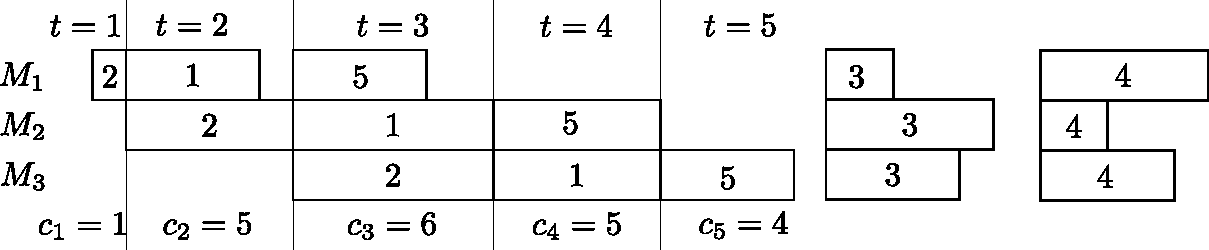
\includegraphics[width=.8\textwidth]{graphics/nfsbsp.pdf}
    \end{center}
    \caption{
        \label{abb:nfsbsp}
        Illustration der Non-Full-Schedule-Heuristik anhand der Beispielinstanz in Tabelle \ref{abb:Bsp}.
        Bislang wurden die Jobs $2$, $1$ und $5$ eingefügt. $3$ und $4$ müssen noch eingefügt werden.
        $2$ wurde zuerst eingefügt, da dieser mit $p_{12}+p_{22}=1+5$ die geringsten $c_+$-Werte auf den ersten $m-1=2$ Maschinen hat.
        $1$ und $5$ wurden eingefügt, weil ihre beiden ersten Prozesszeiten die beiden letzten Zykluszeiten nicht vergrößern.
        Als nächstes wird Job $4$ eingefügt, da weder seine Prozesszeit auf $M_1$ ($p_{14}=5$) die Zykluszeit $c_4=5$ vergrößern würde
        noch seine Prozesszeit auf $M_2$ ($p_{24}=2$) die Zykluszeit $c_5=4$ vergrößern würde.
        Job $3$ hingegen würde mit $p_{23}=5$ die Zykluszeit $c_5=4$ um $1$ vergrößern.
    }
\end{figure}

Da in jeder Iteration alle verbleibenden Jobs betrachtet werden und für jeden dieser Jobs $m-1$ Zeiten verglichen werden,
liegt die asymptotische Laufzeit dieser Heuristik in $\mathcal{O}(n^2m)$.

\subsubsection{Double Ended Non-Full-Schedule-Heuristik}
Diese Heuristik basiert auf der Non-Full-Schedule-Heuristik.
Der Unterschied besteht darin, dass $\pi$ nicht nur von vorne, sondern gleichzeitig auch von hinten zur Mitte hin aufgebaut wird.
Jeder noch nicht in $\pi$ enthaltene Job wird pro Iteration mit beiden Enden der bisherigen Reihenfolge verglichen.
Die Bewertungsfunktion für das hintere Ende arbeitet analog.
Es wird der beste Job für das vordere Ende und der beste für das hintere Ende gesucht und der mit der besseren Bewertung wird vorne bzw. hinten eingefügt.
Die asymptotische Laufzeit liegt hier ebenfalls in $\mathcal{O}(n^2m)$.

\subsubsection{Gilmore-Gomory-Heuristik}
\label{subsubsec:ggHeuristik}
Diese Heuristik wendet den Algorithmus von Gilmore und Gomory auf beliebige Instanzen an.
Es können zwei Fälle eintreten:
\begin{enumerate}
    \item Unter den dominierenden Maschinen $D$ gibt es zwei, die benachbart sind, also $\exists i\in\{1,\ldots,m-1\}$ mit $i,i+1\in D$.
    \item Es gibt keine benachbarten dominierenden Maschinen.
\end{enumerate}
Wenn Fall (2) eintritt, werden alle $m$ Maschinen als dominierend angesehen, da dies für den Algorithmus keine Einschränkung darstellt.
Nun werden zwei benachbarte dominierende Maschinen gewählt.
O.B.d.A seien dies die Maschinen $M_1$ und $M_2$. Seien 
\begin{align} 
    d_{\min} &\coloneqq \min_{\substack{i\in \{1,2\} \\ j\in N}} p_{ij} \\
    e_{\max} &\coloneqq \max_{\substack{i\not\in \{1,2\} \\ j\in N}} p_{ij} \\
    K &\coloneqq \frac{e_{\max}}{d_{\min}} \text{,}
\end{align}
wobei $d_{\min}=0$ und daraus folgend $K=\infty$ erlaubt sind. 
Nun wird aus der gegebenen Instanz $I$ eine neue Instanz $I'$ erzeugt, die sich nur dadurch von $I$ unterscheidet, dass die Prozesszeiten
auf allen dominierenden Maschinen außer auf $M_1$ und $M_2$ mit $\frac{1}{K}$ skaliert werden, also
\begin{align}
    p'_{ij} \coloneqq \begin{cases} \frac{p_{ij}}{K} &\text{für } i\in D\setminus\{1,2\} \\ p_{ij} &\text{sonst.} \end{cases}
\end{align}
Auf diese Weise sind $M_1$ und $M_2$ in $I'$ die einzigen dominierenden Maschinen und folglich kann $I'$ mit dem Algorithmus von Gilmore und Gomory optimal gelöst werden.
Die resultierende Reihenfolge $\pi$ wird als heuristische Lösung für die ursprüngliche Instanz $I$ verwendet.

Da die Prozesszeiten der in $I'$ vernachlässigten dominierenden Maschinen sich um den Faktor $K$ von denen in $I$ unterscheiden, 
können sich die aus $\pi$ ergebenen Zykluszeiten von $I$ und $I'$ auch maximal um den Faktor $K$ unterscheiden:
\begin{align}
    c_t \leq K\cdot c'_t \quad \forall 1\leq t\leq n+m-1
\end{align}
Da die optimale Lösung von $I'$ eine untere Schranke für die optimale Lösung von $I$ ist, also $C'_{\max} \leq C_{\max}$, folgt für die Lösung $L_{GG}$ der
Gilmore-Gomory-Heuristik:
\begin{align}
    L_{GG} \leq K\cdot C'_{\max} \leq K\cdot C_{\max}
\end{align}
Die Gilmore-Gomory-Heuristik hat also eine relative Gütegarantie von $K$.
Bei der Wahl der beiden benachbarten dominierenden Maschinen sollte darauf geachtet werden, dass $d_{\min}$ möglichst groß und $e_{\max}$ möglichst klein ist.
Dadurch ist dann auch der Gütefaktor $K$ am kleinsten.

Das Finden der geeigneten dominierenden Maschinen kann in $\mathcal{O}(nm)$ durchgeführt werden. 
Das Anpassen der Prozesszeiten der übrigen dominierenden Maschinen ist nur in der Theorie von Interesse.
Der Gilmore-Gomory-Algorithmus kann diese einfach ignorieren.
Die Gesamtlaufzeit beträgt daher $\mathcal{O}(nm + n\log n)$.

Für die weitere Analyse dieser Heuristik soll der Begriff der \textit{Semidominanz} eingeführt werden.
Die Semidominanz ist ein Maß dafür, wie weit eine Teilmenge von Maschinen davon entfernt ist, dominierend zu sein.
Eine Semidominanz von $0$ bedeutet, die Maschinen sind dominierend.
Für eine Teilmenge von Maschinen $D\subseteq\{1,\ldots,m\}$ sei 
\[d_{\min} = \min_{\substack{i\in D \\ j\in\{1,\ldots,n\}}} p_{ij}\] 
die kleinste ihrer Prozesszeiten, analog zur obigen Definition von $d_{\min}$.
Die Semidominanz ist dann definiert als
\[\mathcal{D}_{D} \coloneqq \sum_{i\not\in D} \sum_{j=1}^n \max\{0,p_{ij}-d_{\min}\} \text{.}\]
Unabhängig von der \textit{relativen} Gütegarantie $K$ liefert diese Heuristik auch eine \textit{absolute} Gütegarantie von $\mathcal{D}_{\{i,i+1\}}$, 
wenn $M_i$ und $M_{i+1}$ als benachbarte Maschinen ausgewählt werden.
Die Gilmore-Gomory-Heuristik liefert also besonders gute Näherungen, wenn zwei benachbarte Maschinen fast dominierend sind und nur wenige Prozesszeiten auf anderen
Maschinen dies verhindern.

\subsubsection{Nachbarschaftssuche}
\label{subsubsec:Nachbarschaftssuche}
Mit einer Nachbarschaftssuche können bereits existierende (nicht optimale) Reihenfolgen verbessert werden.
Mögliche Nachbarschaftsoperatoren sind
\begin{itemize}
    \item $\mathit{xch}_{jk}$: vertauscht die Jobs an den Positionen $j$ und $k$ miteinander,
    \item $\mathit{shift}_{jk}$: "`shiftet"' den Job an Position $j$ nach Position $k$. 
        Alle Jobs zwischen $j$ und $k$ rücken um eins nach links (falls $j<k$) bzw. nach rechts (falls $j>k$).
\end{itemize}
Auf Grundlage dieser Nachbarschaften lassen sich außerdem z.B. Iterative Improvement, eine Tabu-Suche oder Simulated Annealing implementieren.

Im Rahmen dieser Arbeit wurde ein Simulated Annealing Algorithmus auf Grundlage der $\mathit{xch}_{jk}$-Nachbarschaft implementiert.
Es wird mit einer zufälligen initialen Reihenfolge $\pi$ begonnen.
Die Funktion, die $C_{\max}$ von $\pi$ berechnet, sei mit $c$ bezeichnet.
Pro Iteration werden zufällige $j$ und $k$ bestimmt, mit denen eine benachbarte Lösung $\pi' = \mathit{xch}_{jk}(\pi)$ erzeugt wird.
Ist $\pi'$ besser als die aktuelle Lösung $\pi$, d.h. $c(\pi') < c(\pi)$, wird $\pi'$ als neue Lösung übernommen.
Ist $\pi'$ schlechter als $\pi$, wird $\pi'$ nur mit einer bestimmten Wahrscheinlichkeit übernommen.
Diese Wahrscheinlichkeit beträgt $e^{\frac{c(\pi)-c(\pi')}{t_i}}$, wobei $(t_i)_i$ eine Nullfolge ist 
und $i$ die Anzahl der bisher durchgeführten Iterationen angibt.
Die Folge $(t_i)_i$ wird auch als "`Temperatur"' bezeichnet, die im Laufe des Verfahrens abnimmt.
Es wurde mit unterschiedlichen Temperaturen experimentiert.
Es wurden 
\begin{itemize}
    \item $t_i = \alpha t_{i-1}$ für unterschiedliche $\alpha\in]0,1[$ und 
    \item $t_i = \frac{k}{i}$, 
    \item $t_i = \frac{k}{\log i}$ und 
    \item $t_i = k \frac{|\cos\frac{i}{30}|}{i}$
\end{itemize}
jeweils für unterschiedliche $k\in\mathbb{R}_+$ getestet. Die besten Resultate lieferte $t_i = 50\frac{|\cos\frac{i}{30}|}{i}$.
Durch den Cosinus schwankt die Temperatur, so dass abwechselnd verschlechternde Lösungen erlaubt bzw. nicht erlaubt werden.
Das Verfahren terminiert, sobald in 1000 aufeinander folgenden Iterationen keine neue beste Lösung gefunden werden konnte.

Dieser Simulated Annealing Algorithmus lieferte in Tests meist etwas bessere Ergebnisse als die übrigen Heuristiken.
Die Heuristiken werden in Kapitel \ref{chap:RechenergebnisseUndVergleiche} verglichen.

\subsubsection{Heuristiken von Soylu et al.}
Die oben beschriebenen Heuristiken werden in Kapitel \ref{chap:RechenergebnisseUndVergleiche} nicht nur untereinander verglichen, 
sondern auch mit drei Heuristiken von Soylu et al. \cite{soylu}, die hier kurz beschrieben werden.

\paragraph{$H_1$}
Diese Heuristik erstellt $m$ unterschiedliche Jobreihenfolgen und wählt anschließend die beste aus.
Die $k$-te dieser $m$ Reihenfolgen wird erstellt, indem für die Zyklen $k,\ldots,n+k-1$ die Anzahl der Jobs betrachtet wird,
die sich in diesem Zyklus in der Anlage befinden (diese Anzahl beträgt nur in den ersten und letzten $m-1$ Zyklen \textit{nicht} $m$).
Anschließend werden die Jobs den Zyklen so zugewiesen, dass der Job mit der $i$-t kleinsten Prozesszeit im Zyklus mit der $i$-t kleinsten Anzahl an Jobs liegt.
Es werden also $m-1$ Jobs einer wohldefinierten Position in $\pi$ zugewiesen (nämlich den Zyklen, in denen weniger als $m$ Jobs in der Anlage sind) 
und die übrigen $n-m$ Jobs werden wahllos eingefügt, da alle übrigen Zyklen $m$ Jobs enthalten und somit bezüglich dieser Metrik nicht unterscheidbar sind.

\paragraph{$H_2$}
Hier wird in einer Iteration ein Job in die anfangs leere Reihenfolge eingefügt.
Es wird unter allen noch nicht eingefügten Jobs jeweils derjenige ausgesucht, der die größte Prozesszeit hat.
Dieser Job wird dann so in die Reihenfolge eingefügt, dass diese Prozesszeit in den Zyklus fällt, dessen Zykluszeit bislang am größten war.
Sollte das nicht möglich sein, wird stattdessen die zweitgrößte Zykluszeit gewählt usw.
Auf diese Weise werden alle Jobs nacheinander eingefügt. 
Der erste Job, der die größte aller Prozesszeiten hat, wird so eingefügt, dass diese Prozesszeit in Zyklus $m$ liegt.

\paragraph{$H_3$}
Diese Heuristik ähnelt der Non-Full-Schedule-Heuristik (vgl. Abschnitt \ref{subsubsec:NonFullScheduleHeuristik}).
Der Unterschied besteht darin, dass zu der Summe der $c_+$-Werte noch die Prozesszeit auf der letzten Maschine des jeweiligen Jobs mit aufaddiert wird
und diese Gesamtsumme dann als Einfügekriterium dient.
Sollte es mehrere gleichwertige Jobs geben, wird kein zweites Kriterium zu Rate gezogen, sondern zufällig einer ausgewählt.


\section{Zuweisung von Ressourcen}
\label{sec:ZuweisungVonRessourcen}
In diesem Abschnitt geht es darum, den Jobs in der Reihenfolge $\pi$, die in Abschnitt \ref{sec:BerechnenEinerJobreihenfolge} aufgestellt wurde,
Ressourcen zuzuweisen. An diese Zuweisung werden zwei Anforderungen gestellt:
\begin{enumerate}
    \item Die Zuweisung muss zulässig sein. Das heißt, ist eine Ressource einem Job zugewiesen, darf sie den nachfolgenden $m-1$ Jobs nicht mehr zugewiesen werden.
        Das Problem der Zulässigkeit einer Zuweisung wird im ersten Unterabschnitt \ref{subsec:ZulaessigkeitDerZuweisung} betrachtet.
    \item Die Zuweisung soll möglichst gut sein. Wenn zwei Jobs, die im Abstand von $m$ in $\pi$ liegen, die selbe Ressource benutzen können,
        werden Rüstkosten eingespart, da die Ressource nicht ausgetauscht werden muss.
        Dieses Problem wird in Unterabschnitt \ref{subsec:OptimierungDerRessourcenzuweisung} diskutiert.
\end{enumerate}
Es ist natürlich möglich, dass bei gegebenem $\pi$ keine zulässige Zuweisung von Ressourcen möglich ist.
In diesem Fall muss $\pi$ nachträglich geändert werden, worauf in Unterabschnitt \ref{sec:UnzulaessigeReihenfolgen} eingegangen wird.

\subsection{Zulässigkeit der Zuweisung}
\label{subsec:ZulaessigkeitDerZuweisung}
Abhängig davon, welche Ressourcen für welche Jobs geeignet sind, kann das Zulässigkeitsproblem unterschiedlich schwer zu lösen sein.
Folgende Situationen werden hier betrachtet:
\begin{itemize}
    \item Alle Ressourcen sind für alle Jobs geeignet (trivial, es müssen $m$ Ressourcen vorhanden sein).
    \item Die Ressourcenmengen sind disjunkt ($\rho_i\cap\rho_j \neq \emptyset \enspace \Rightarrow \enspace \rho_i = \rho_j$).
    \item Die $\rho_i$ sind beliebige Teilmengen von $R$.
\end{itemize}
Der Fall, dass die Ressourcen für hierarchische Jobgruppen geeignet sind 
($\iota_q\cap\iota_r \neq \emptyset \enspace \Rightarrow \enspace \iota_q\subseteq\iota_r$ oder $\iota_r\subseteq\iota_q$),
wird nicht gesondert betrachtet.
Da dieser Fall aber natürlich auch ein Spezialfall der beliebigen Teilmengen ist, kann er mit demselben Verfahren gelöst werden.

\subsubsection{Zulässigkeit bei disjunkten Ressourcenmengen}
\label{subsubsec:ZulaessigkeitBeiDisjunktenRessourcenmengen}
Bei disjunkten Ressourcenmengen können die Jobs in Gruppen unterteilt werden, 
so dass zu jeder Jobgruppe eine für sie exklusive Menge an zulässigen Ressourcen zur Verfügung steht.
Für die Zulässigkeit reicht es aus, statt der Ressourcenmengen $\rho_i$ nur deren Größen $|\rho_i|$ zu betrachten.
Mit einem Greedy-Algorithmus kann eine gegebene Reihenfolge $\pi$ dann auf Zulässigkeit überprüft werden:
Der Algorithmus durchläuft $\pi$ von vorne nach hinten.
Jede Jobgruppe erhält einen Counter, der mitzählt, wie viele Ressourcen momentan für sie zur Verfügung stehen.
Diese Counter werden zu Beginn mit $|\rho_i|$ initialisiert.
An jeder Position in $\pi$ wird der Counter der zugehörigen Jobgruppe dekrementiert.
Nach $m$ Schritten wird dieser Counter wieder inkrementiert.
Sollte ein Counter einmal negativ werden, gibt es keine zulässige Ressourcenzuteilung.

%\subsubsection{Zulässigkeit bei hierarchischen Jobgruppen}
%Diese Situation kann mit einem ähnlichen Greedy-Algorithmus gelöst werden, wie bei disjunkten Ressourcenmengen.
%Die Ressourcen, die für eine Jobgruppe geeignet sind, können hier allerdings nicht als identisch angesehen werden,
%so dass es genügen würde, wieder nur die Anzahl der Ressourcen zu betrachten.
%Die Ressourcen unterscheiden sich dahingehend voneinander, dass sie für unterschiedlich viele andere Jobs ebenfalls geeignet sind.
%Der Greedy-Algorithmus muss so abgeändert werden, dass er jedem Job in $\pi$ immer die "`speziellste"' aktuell für diesen Job verfügbare Ressource zuweist.
%Soll einem Job $j$ eine Ressource zugeteilt werden, muss unter allen geeigneten Ressourcen $r\in\rho_j$, 
%wobei $r$ nicht schon einem anderen Job zugewiesen sein darf, diejenige mit minimalem $|\iota_r|$ ausgesucht werden.
%
%Dieser abgewandelte Greedy-Algorithmus ist korrekt, denn immer, wenn die Situation auftritt, dass für einen Job $j$ keine Ressource verfügbar ist,
%liegt das daran, dass alle potentiell geeigneten Ressourcen $\rho_j$ bereits an einen der $m-1$ direkten Vorgänger von $j$ vergeben worden sind.
%Sei $f$ das unvollständige Mapping, das der Algorithmus bis zu diesem Punkt aufgestellt hat.
%Sei $F\subseteq N$ die Menge der Vorgänger von $j$, denen eine Ressource $r\in\rho_j$ zugeteilt wurde.
%Angenommen, es existiert ein zulässiges Mapping $f'$, obwohl der Algorithmus $j$ keine Ressource zuweisen kann.
%Dann muss es einen Job $i\in F$ geben mit $f'(i)\not\in\rho_j$.
%Wegen der hierarchischen Eigenschaft muss entweder $\iota_{f'(i)}\subset\iota_{f(i)}$ sein oder $\iota_{f(i)}\subseteq\iota_{f'(i)}$.
%Da $f(i)\not\in\rho_j$ ist (und somit auch $j\not\in\iota_{f'(i)}$),
%muss hier $\iota_{f'(i)}\subset\iota_{f(i)}$ sein, denn sonst wäre $j\in\iota_{f(i)}\subseteq\iota_{f'(i)}$.
%Das wiederum bedeutet, dass auch der Algorithmus dem Job $i$ die speziellere Ressource $f'(i)$ zugewiesen hätte.
%Da er das aber nicht getan hat, muss er sie stattdessen einem der $m-1$ direkten Vorgänger von $i$ zugewiesen haben.
%Sei $h$ dieser Vorgänger von $i$.
%Es ist also $f(h)=f'(i)$ und somit $f'(h)\neq f'(i)$.


\subsubsection{Zulässigkeit bei beliebigen Ressourcenteilmengen}
\label{subsubsec:ZulaessigkeitBeiBeliebigenRessourcenteilmengen}
Es ist nicht bekannt, ob das Problem, zu entscheiden, ob es bei gegebenem $\pi$ und beliebigen Ressourcenmengen ein zulässiges Mapping $f$ gibt, 
$\mathcal{NP}$-vollständig ist oder ob es einen polynomiellen Algorithmus gibt.

Es besteht allerdings die Vermutung, dass es bei konstantem $m$ einen polynomiellen Algorithmus in $n$ gibt. Ein Indiz für diese Vermutung liefert das nachfolgende MIP.
O.B.d.A. sei hier $\pi_i=i$, d.h. Job $i$ ist an Position $i$.
Die Binärvariablen $x_{ir}$ geben hier an, ob dem Job $i\in N$ die Ressource $r\in\rho_i$ zugeteilt wird.
In diesem Fall ist $x_{ir}=1$ und sonst $x_{ir}=0$.
\begin{align}
    \text{max} \quad &0 \label{zulmip:obj} \\
    \text{s.t.}\quad \sum_{r\in\rho_i} x_{ir} &= 1 & i\in N \label{zulmip:1} \\
    x_{ir} + x_{jr} &\leq 1 & i\in N, j=i+1,\ldots,i+m-1 \, ,r\in\rho_i\cap\rho_j \label{zulmip:2} \\
    x_{ir} &\in \{0,1\} & i\in N, r\in\rho_i
\end{align}
Die erste Nebenbedingung (\ref{zulmip:1}) bewirkt, dass jedem Job genau eine Ressource zugewiesen wird.
Durch die zweite Nebenbedingung (\ref{zulmip:2}) kann jede Ressource jeweils nur einmal an $m$ aufeinander folgende Jobs vergeben werden.
Eine Zielfunktion ist nicht notwendig, da die Zulässigkeit nur durch die Nebenbedingungen entschieden wird.
Mit diesem MIP können selbst sehr große Instanzen mit $n\approx 100000$ (allerdings mit $m\leq 8$) in weniger als einer Sekunde gelöst werden.

Nebenbedingung (\ref{zulmip:2}) verhindert immer nur für Paare von Jobs, deren Abstand kleiner als $m$ ist, dass ihnen die selbe Ressource zugewiesen wird.
Das ist für die Korrektheit des MIPs zwar ausreichend, durch zusätzliche Nebenbedingungen, die dasselbe für Tripel, Quadrupel, bis hin zu $m$-Tupeln verhindern,
können aber einige fraktionale Lösungen der Relaxation "`abgeschnitten"' werden.
Für ein $k$-Tupel von Jobs, die alle in einem Abschnitt von $\pi$ der Länge $m$ stehen, sieht diese zusätzliche Nebenbedingung so aus:
\begin{align}
    \sum_{l=1}^k x_{i_lr} \leq 1 \quad i_l\in N, i_1<i_2<\ldots<i_k<i_1+m, r\in\bigcap_{l=1}^k \rho_{i_l}
\end{align}
Für $k=2$ ist diese Nebenbedingung identisch mit (\ref{zulmip:2}).
Die Anzahl dieser Nebenbedingungen lässt sich durch $\mathcal{O}(n(m-1)!|R|)$ abschätzen, was bei konstantem $m$ polynomiell ist.
Werden sie für $k=3,\ldots,m$ zu obigem MIP hinzugefügt, so war bei allen bislang getesteten 100 Instanzen die Relaxation bereits ganzzahlig.
Ein Beweis, dass dies tatsächlich bei allen Instanzen der Fall ist, ist noch nicht gelungen.
Gelingt er, ist bewiesen, dass es in polynomieller Zeit (bei konstantem $m$) möglich ist, zu entscheiden, ob es für eine gegebene Jobreihenfolge $\pi$ und 
gegebene (beliebige) Ressourcenteilmengen $\rho_i$ möglich ist, allen Jobs eine Ressource zuzuweisen.


\subsection{Optimierung der Ressourcenzuweisung}
\label{subsec:OptimierungDerRessourcenzuweisung}
Da unbekannt ist, ob das Finden \textit{irgendeiner} zulässigen Ressourcenzuweisung $\mathcal{NP}$-schwer ist,
ist es natürlich ebenfalls unbekannt, ob das Finden einer \textit{optimalen} Ressourcenzuweisung $\mathcal{NP}$-schwer ist.

Eine Ausnahme bildet der Fall von disjunkten Ressourcenteilmengen $\rho_i$.
Immer, wenn zwei Jobs aus einer Familie im Abstand $m$ aufeinander folgen, kann ihnen dieselbe Ressource zugewiesen werden.
Wenn zwei Jobs im Abstand $m$ nicht zur selben Familie gehören, gibt es auch keine Möglichkeit, Rüstkosten zu vermeiden oder zu verringern.

Für den allgemeinen Fall lässt sich das MIP aus Unterabschnitt \ref{subsubsec:ZulaessigkeitBeiBeliebigenRessourcenteilmengen} erweitern.
Hinzu kommen für $i\in \{m+1,\ldots,n\}$ und $r\in\rho_i\cap\rho_{i-m}$ Binärvariablen $y_{ir}$, für die gilt: 
$y_{ir}=1$ genau dann, wenn den Jobs an den Positionen $i$ und $i-m$ in $\pi$ die selbe Ressource $r$ zugeteilt ist.
Auch hier sei wieder o.B.d.A. $\pi_i=i$.
\begin{align}
    \text{max} \quad \sum_{i=m}^n\sum_{r\in\rho_i\cap\rho_{i-m}} &y_{ir} \label{optmip:obj} \\
    \text{s.t.}\quad \sum_{r\in\rho_i} x_{ir} &= 1 & i\in N \label{optmip:1} \\
    x_{ir} + x_{jr} &\leq 1 & i\in N, j=i+1,\ldots,i+m-1 \, ,r\in\rho_i\cap\rho_j \label{optmip:2} \\
    y_{ir} &\leq x_{ir} & i=m,\ldots,n \, ,r\in\rho_i\cap\rho_{i-m} \label{optmip:3}\\
    y_{ir} &\leq x_{i-m,r} & i=m,\ldots,n \, ,r\in\rho_i\cap\rho_{i-m} \label{optmip:4}\\
    x_{ir} &\in \{0,1\} & i\in N, r\in\rho_i \\
    y_{ir} &\in \{0,1\} & i=m,\ldots,n \, ,r\in\rho_i\cap\rho_{i-m}
\end{align}
Durch die Nebenbedingungen (\ref{optmip:3}) und (\ref{optmip:4}) wird erzwungen, dass die $y_{ir}$ die oben beschriebenen Werte annehmen.
In der Zielfunktion (\ref{optmip:obj}) wird die Anzahl der $y$-Variablen, die auf $1$ gesetzt sind, maximiert, da so die wenigsten Rüstkosten auftreten.
Dieses MIP liefert genau wie jenes aus \ref{subsubsec:ZulaessigkeitBeiBeliebigenRessourcenteilmengen} in weniger als einer Sekunde auch für sehr große Instanzen eine Lösung.
%Dieser Umstand lässt vermuten, dass auch das Optimierungsproblem der Ressourcenzuteilung in polynomieller Zeit lösbar ist.

\section{Unzulässige Reihenfolgen}
\label{sec:UnzulaessigeReihenfolgen}
Für den Fall, dass für eine gegebene Reihenfolge $\pi$ kein zulässiges Mapping $f$ erstellt werden kann, muss $\pi$ nachträglich verändert werden.

%\subsection{Nachbarschaftssuche}
Eine Nachbarschaftssuche ist eine Möglichkeit zur nachträglichen Änderung von $\pi$:
Mit einer Vertauschung zweier Jobs kann $\pi$ unter Umständen so abgeändert werden, dass doch ein zulässiges Mapping existiert.
Es wird dazu eine Matrix erstellt, deren Einträge $r_{ij}$ angeben, wie viele Ressourcen für Job $j$ an Position $i$ in $\pi$ zur Verfügung stehen
(d.h. sich nicht gerade in der Anlage befinden).
Initial ist $r_{ij}=|\rho_j|$ für alle Positionen $i$.
Indem für alle $i$ die $m$ zuletzt eingelegten Jobs $j$ ermittelt werden (also die an den Positionen $i-m+1,\ldots,i$),
können jeweils die Einträge $r_{ij}$ um $1$ verringert werden.
Sobald einer der Einträge negativ wird, bedeutet das, dass eine Ressource zugewiesen wurde, obwohl sie an dieser Position $i$ nicht mehr verfügbar ist.
Es kann dann ein Job $j'$ an einer anderen Position in $\pi$ gesucht werden, dessen Ressource an Position $i$ noch verfügbar ist.
Dafür muss $r_{ij'}>0$ sein.
Wenn solch ein Job existiert, wird er mit dem Job an Position $i$ getauscht und die Matrix wird angepasst.
Falls mehrere solcher Jobs existieren, wird derjenige ausgewählt, durch dessen Tausch sich die Summe der Zykluszeiten am wenigsten verschlechtert.\footnote{
Es ist nicht ausgeschlossen, dass sich die Summe der Zykluszeiten dadurch sogar verbessert.}
Sollte kein solcher Job gefunden werden, terminiert die Nachbarschaftssuche mit dem Ergebnis, dass kein zulässiges Mapping gefunden werden konnte.
Dabei ist zu beachten, dass dieser Algorithmus nicht garantiert, ein zulässiges Mapping zu finden, falls eines existiert.


%\subsection{Idle-Jobs}
%Falls mit der Nachbarschaftssuche keine Lösung gefunden werden kann, besteht die Möglichkeit sogenannte Idle-Jobs in $\pi$ einzufügen.
%Idle-Jobs sind Jobs, die auf allen Maschinen die Prozesszeit $0$ haben und keine Ressourcen benötigen.
%In der Praxis kann ein Idle-Job durch "`nichts"' realisiert werden, es wird also einfach kein Job in die Station eingelegt.
%Nach dem Einfügen eines Idle-Jobs kann erneut die Nachbarschaftssuche angewandt werden.
%Es können so lange Idle-Jobs eingefügt werden, bis eine gültige Ressourcenzuweisung gefunden wurde.



\chapter{Der zweite Dekompositionsansatz}
\label{chap:DerZweiteDekompositionsansatz}
In diesem Kapitel wird der zweite Dekompositionsansatz vorgestellt.
Hierbei wird erst jedem Job eine Ressource zugewiesen, also ein Mapping $f$ erzeugt,
und anschließend werden die Jobs in eine Reihenfolge $\pi$ gebracht.
Neben der reinen Ressourcenzuteilung wird im ersten Schritt auch teilweise schon festgelegt, welche Jobs in der späteren Reihenfolge einen Abstand von $m$ haben sollen.
So wird sichergestellt, dass die durch das Mapping $f$ vorgeschriebenen Ressourcenzuteilungen auch dazu führen, dass Rüstkosten eingespart werden.

In Abschnitt \ref{sec:Ressourcenzuweisung} wird erklärt, wie ein optimales Mapping $f$ mit möglichst wenigen Rüstkosten mit einem Binpacking-Ansatz erstellt werden kann.
Anschließend wird in Abschnitt \ref{sec:AnordnungDerJobgruppen} beschrieben, wie basierend auf dem gegebenen Mapping $f$ eine Reihenfolge $\pi$ erstellt wird,
so dass die Summe der Zykluszeiten und Rüstkosten ($C_{\max}$) minimal ist.

In den meisten nachfolgend genannten Verfahren wird nur der Spezialfall mit konstanten Rüstkosten ($s_{fg}=s$),
disjunkten Ressourcenmengen $\rho_i$ und zwei dominierenden Maschinen betrachtet
vor dem Hintergrund des gegebenen Praxisbeispiels des Küchenherstellers.


\section{Ressourcenzuweisung}
\label{sec:Ressourcenzuweisung}
In diesem Abschnitt wird die Konstruktion des Mappings $f$ erläutert.
Dabei wird davon ausgegangen, dass Rüstkosten einzig durch einen Ressourcenwechsel verursacht werden.
In Unterabschnitt \ref{subsec:RessourcenzuweisungMitBinpacking} wird auf den Spezialfall $s_{fg}=s$, der mit einem Binpacking-Ansatz gelöst werden kann,
eingegangen. Allgemeinere Fälle der Ressourcenzuweisung beim zweiten Dekompositionsansatz werden in dieser Arbeit nicht gesondert betrachtet.

Wie in Abschnitt \ref{sec:Problembeschreibung} erläutert, ist im Folgenden von \textit{Jobgruppen} die Rede, 
wobei eine Jobgruppe $g$ aus $n_g\in\mathbb{N}$ identischen Jobs besteht.
$n_g$ ist also die Größe einer Jobgruppe $g$.
Die Anzahl der Jobgruppen wird mit $\tilde{n}$ bezeichnet.
Für die Gesamtanzahl an Jobs gilt dann $n = \sum_{g=1}^{\tilde{n}} n_g$.

%\subsection{Bekannte Laufzeitschranken und Verfahren}
%\label{subsec:BekannteLaufzeitschrankenUndVerfahren}

\subsection{Ressourcenzuweisung mit Binpacking}
\label{subsec:RessourcenzuweisungMitBinpacking}
Bei $\tilde{n}$ gegebenen Jobgruppen, wobei alle Jobs aus einer Gruppe die gleichen Ressourcen verwenden können,
ist es naheliegend, die Jobs einer Gruppe immer im Abstand von $m$ in die Anlage einzulegen.
Auf diese Weise muss die Ressource in der entsprechenden Station so lange nicht ausgetauscht werden,
bis alle Jobs aus einer Jobgruppe fertiggestellt worden sind.
Erst danach, wenn Jobs aus einer anderen Gruppe eingelegt werden, muss einmalig die Ressource gewechselt werden,
so dass nur dann Rüstkosten auftreten.
Insgesamt muss dann nur $(\tilde{n}-m)$-mal ein Ressourcenwechsel stattfinden 
(beim Einlegen der ersten $m$ Jobs muss keine Ressource gewechselt werden, evtl. treten aber initiale Rüstkosten auf, was in dieser Arbeit aber nicht beachtet wird).
Dabei soll nur der Spezialfall mit disjunkten Ressourcenmengen und konstanten Rüstkosten ($s_{fg}=s$) betrachtet werden.

Zur Vereinfachung wird angenommen, dass $n$ ein Vielfaches von $m$ ist. 
Bei $\tilde{n}$ gegebenen Jobgruppen mit den Größen $n_g, \, g=1,\ldots,\tilde{n}$ ist das Ziel,
die Jobgruppen in $m$ gleichgroße Teilmengen zu unterteilen, möglichst ohne eine der Jobgruppen zu teilen.
Dieses Problem lässt sich als Binpacking-Instanz betrachten, wobei entschieden werden muss, ob $\tilde{n}$ Items 
mit den Größen $n_1,\ldots,n_{\tilde{n}}$ in $m$ Bins der Größe $\frac{n}{m}$ untergebracht werden können.
Jobs, die sich in einem Bin befinden, werden danach einer Station der Anlage zugewiesen.
Da eine Station sich nach genau $m$ Zyklen wieder an ihrer Ausgangsposition befindet,
werden die Jobs eines Bins immer im Abstand von $m$ in die Anlage eingelegt und wenn sie zur gleichen Jobgruppe gehören, treten keine Rüstkosten auf,
da die Ressource in der Station bleiben kann.

Für den Fall, dass die Binpacking-Instanz eine Lösung hat, müssen noch die Bins den Stationen zugeordnet werden und die Reihenfolge
der Jobgruppen in jedem Bin muss so bestimmt werden, dass die Zykluszeiten minimiert werden.
Dies wird in Abschnitt \ref{sec:AnordnungDerJobgruppen} beschrieben.
Falls die Binpacking-Instanz keine Lösung hat, bedeutet das, dass mindestens eine der Jobgruppen aufgeteilt werden muss auf zwei Bins,
so dass ein weiteres Mal Rüstkosten auftreten.

Um herauszufinden, welche Jobgruppe geteilt werden muss und wie groß die beiden Hälften sein müssen,
wird eine weitere Binpacking-Instanz\footnote{Streng genommen handelt es sich hierbei nicht mehr um eine Binpacking-Instanz wegen der unterschiedlichen Bingrößen.} 
gelöst, die bis auf eine Änderung identisch zur vorherigen ist:
Es gibt nicht mehr $m$ Bins, sondern nur noch $m-1$ und einer dieser Bins hat die Größe $2\frac{n}{m}$ (alle anderen haben weiterhin die Größe $\frac{n}{m}$).
Wenn hier eine Aufteilung möglich ist, kann der Bin mit doppelter Größe wieder halbiert werden,
wobei dann eine der Jobgruppen in ihm auch geteilt werden muss wie in Abbildung \ref{abb:2binbsp} veranschaulicht.
Sollte auch hier keine Lösung möglich sein, muss eine weitere Jobgruppe geteilt werden.
Dazu wird wiederum eine neue Binpacking-Instanz erzeugt.
Abbildung \ref{abb:binpart} zeigt, wie die Bingrößen in den weiteren Instanzen aussehen.
Es handelt sich dabei um die \textit{ungeordneten Zahlenpartitionen} von $m$.
Spätestens bei der Binpacking-Instanz, die nur noch einen Bin enthält mit der Größe $n$, gibt es eine Lösung,
bei der dann $m-1$ Jobgruppen aufgeteilt werden müssen, so dass $m-1$ weitere Ressourcenwechsel und damit Rüstkosten auftreten.
\begin{figure}
    \begin{center}
        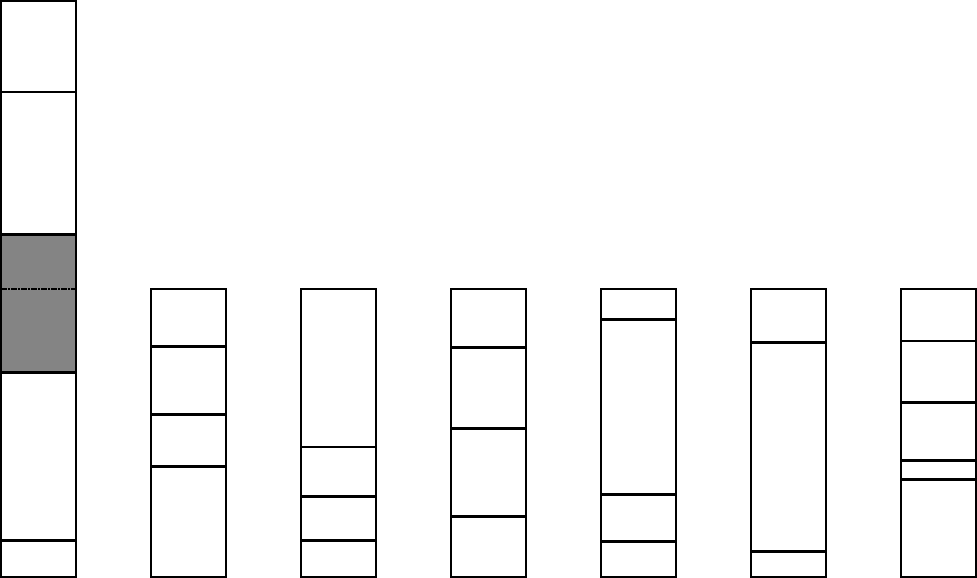
\includegraphics[width=.6\textwidth]{graphics/2binbsp.pdf}
    \end{center}
    \caption{
        \label{abb:2binbsp}
        Jobgruppen, die $m=8$ Bins zugeordnet werden.
        Da die ursprüngliche Binpacking-Instanz keine Lösung hatte, wurden zwei der Bins zu einem mit doppelter Größe verschmolzen.
        Auf diese Weise ist es möglich, die Jobgruppen passgenau zuzuordnen, wobei die grau markierte Jobgruppe
        getrennt werden muss und im Folgenden als zwei Jobgruppen angesehen wird.
    }
\end{figure}
\begin{figure}
    \begin{center}
        \begin{tabular}{cccccccc}
            1 & 1 & 1 & 1 & 1 & 1 & 1 & 1  \\ \hline
            2 & 1 & 1 & 1 & 1 & 1 & 1 & \\ \hline
            2 & 2 & 1 & 1 & 1 & 1 & &\\
            3 & 1 & 1 & 1 & 1 & 1 & &\\ \hline
            2 & 2 & 2 & 1 & 1 & & &\\
            3 & 2 & 1 & 1 & 1 & & &\\
            4 & 1 & 1 & 1 & 1 & & &\\ \hline
            2 & 2 & 2 & 2 & & & &\\
            3 & 2 & 2 & 1 & & & &\\
            3 & 3 & 1 & 1 & & & &\\
            4 & 2 & 1 & 1 & & & &\\
            5 & 1 & 1 & 1 & & & &\\ \hline
            3 & 3 & 2 & & & & &\\
            4 & 2 & 2 & & & & &\\
            4 & 3 & 1 & & & & &\\
            5 & 2 & 1 & & & & &\\
            6 & 1 & 1 & & & & &\\ \hline
            4 & 4 & & & & & &\\
            5 & 3 & & & & & &\\
            6 & 2 & & & & & &\\
            7 & 1 & & & & & &\\ \hline
            8 & & & & & & &
        \end{tabular}
    \end{center}
    \caption{
        \label{abb:binpart}
        Ungeordnete Zahlenpartitionen von $8$ bezüglich $m'$ gruppiert und sortiert.
        Jede Zeile stellt die Anzahl der Bins und deren Größe bei möglichen Binpacking-Instanzen dar.
        Die zweite Zeile beispielsweise stellt den Status der Instanz in Abbildung \ref{abb:2binbsp} dar.
    }
\end{figure}

Da das Binpacking-Problem in der hier dargebotenen Form nur schwach $\mathcal{NP}$-vollständig in der Anzahl der Jobgruppen $\tilde{n}$ ist,
lässt es sich trotzdem (theoretisch) polynomiell in der Eingabegröße $n$ lösen.
Im Rahmen dieser Arbeit wurde das nachfolgende MIP aufgestellt, um die Jobgruppen den Bins zuzuordnen.
%Das Binpacking-Problem ist zwar $\mathcal{NP}$-vollständig, da aber sowohl die Anzahl der Bins $m$ 
%als auch die Anzahl der Items bzw. Jobgruppen $\tilde{n}$ meist relativ klein sind (meist deutlich kleiner als die Anzahl Jobs $n$),
%lässt sich das Problem, die Jobgruppen den Bins zuzuordnen und ggf. geeignete Jobgruppen zu finden, die aufgeteilt werden müssen, 
%trotzdem in hinnehmbarer Zeit mit dem nachfolgenden MIP lösen. 
Für die Binärvariablen $x_{gj}$ gilt: $x_{gj}=1$ genau dann, wenn Jobgruppe $g$ Bin $j$ zugeordnet wird.
Die erste Nebenbedingung fordert, dass jede Jobgruppe in genau einem Bin ist 
und die zweite Nebenbedingung verlangt, dass jeder Bin exakt gefüllt ist.
Dabei sind $B_j$ die Größen der Bins, die zusammen mit der Anzahl der Bins $m'$ mit jedem Aufruf einer Zahlenpartition von $m$ entsprechen:
\begin{align}
    \text{max} \quad &0 \\
    \text{s.t.}\quad \sum_{j=1}^{m'} x_{gj} &= 1 &g=1,\ldots,\tilde{n}\\
    \sum_{g=1}^{\tilde{n}} n_g x_{gj} &= B_j &j=1,\ldots,m' \\
    x_{gj} &\in \{0,1\} &g=1,\ldots,\tilde{n}, \, j=1,\ldots,m'
\end{align}
%In Abbildung \ref{abb:binzeit} sind die Laufzeiten dieses MIPs aufgetragen.
%Dabei wurde das MIP in ZIMPL formuliert und mit CPLEX gelöst.
Die Partitionen von $m$ wurden der Reihenfolge nach (vgl. Abbildung \ref{abb:binpart}) mit kleiner werdendem $m'$ durchlaufen,
bis eine zulässige Aufteilung gefunden wurde.


\subsection{Zulässigkeit der Zuweisung}
\label{subsec:ZulaessigkeitDerZuweisung}
In Unterabschnitt \ref{subsec:RessourcenzuweisungMitBinpacking} wurde erläutert, wie Jobs bzw. Jobgruppen so angeordnet werden können,
dass möglichst selten eine Ressource gewechselt werden muss, was Rüstkosten verursacht.
Es wurde allerdings davon ausgegangen, dass immer genug Ressourcen vorhanden sind,
d.h. es wurde nur optimiert, ohne zu beachten, ob diese Zuweisung von Ressourcen überhaupt zulässig ist.
Für den Fall der disjunkten Ressourcenmengen wird im Folgenden beschrieben, unter welchen Umständen die Lösung des Binpackings zulässig ist
bezüglich der vorhandenen Ressourcen.
Dazu wird zunächst beschrieben unter welchen Voraussetzungen eine Unzulässigkeit überhaupt nur auftreten kann.
Anschließend wird erläutert, wie selbst dann teilweise doch noch Zulässigkeit erreicht werden kann.

\subsubsection{Voraussetzungen für Unzulässigkeit}
O.B.d.A. kann davon ausgegangen werden, dass es für jede Jobgruppe mindestens eine zulässige Ressource gibt.
Andernfalls könnten diese Jobs niemals produziert werden.
Unzulässigkeit tritt genau dann auf, wenn weniger Ressourcen für eine Jobgruppe $g$ vorhanden sind als sich Jobs aus $g$ gleichzeitig in der Anlage befinden.
Grundvoraussetzung dafür ist, dass $g$ beim Binpacking auf mehrere Bins aufgeteilt wurde.
Ist dies nicht der Fall, werden die Jobs aus $g$ immer im Abstand von $m$ in die Anlage eingelegt,
so dass nur genau eine Ressource benötigt wird, um alle Jobs aus $g$ zu produzieren.
Eine Jobgruppe, die nicht geteilt wird, kann also keine Unzulässigkeit verursachen.
Es müssen daher nur geteilte Jobgruppen betrachtet werden, von denen es maximal $m-1$ geben kann
(wenn die letzte Binpacking-Instanz mit nur noch einem Bin der Größe $n$ erreicht wurde).

\begin{figure}
    \begin{center}
        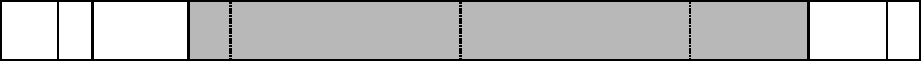
\includegraphics[width=.8\textwidth]{graphics/kteilung.pdf}
    \end{center}
    \caption{
        \label{abb:kteilung}
        Ein Bin der Größe $4\frac{n}{m}$ (ein $4$-Bin) mit $6$ Jobgruppen, von denen eine so groß ist,
        dass sie an drei Stellen geteilt werden muss.
        Alle mittleren Teilstücke haben dann die Größe $\frac{n}{m}$ und die Größen der beiden äußeren
        Teilstücke liegen im Intervall $[1,\frac{n}{m}]$.
    }
\end{figure}
Nun soll der Fall betrachtet werden, dass eine Jobgruppe mehrfach geteilt wurde 
(die Gesamtanzahl von Teilungen von allen Jobgruppen zusammen kann höchstens $m-1$ betragen).
Eine Jobgruppe $g$ kann nur dann mehr als einmal geteilt werden, wenn $n_g > \frac{n}{m}$ ist.
Bei einer $k$-fachen Teilung von $g$ gilt für die resultierenden Teilgruppen $n_{g_1},n_{g_k}\leq\frac{n}{m}$ und $n_{g_i}=\frac{n}{m}$ für $i=2,\ldots,k-1$
(vgl. Abbildung \ref{abb:kteilung}).
Allen Teilgruppen mit $g_i=\frac{n}{m}$ kann eine Ressource fest zugeteilt werden, da sich Jobs dieser Teilgruppen durchgehend auf einer Station befinden.
Sie können daher als eigenständige Jobgruppen mit genau einer zulässigen Ressource aufgefasst werden.
Für $g_1$ und $g_k$ stehen dann entsprechend weniger Ressourcen zur Verfügung.
Daher kann o.B.d.A. davon ausgegangen werden, dass jede Jobgruppe höchstens einmal geteilt werden kann, d.h. $k\leq 1$.

Die Lösung des Binpackings kann also nur dann unzulässig sein, wenn es für eine Jobgruppe $g$, die geteilt wird, nur eine Ressource gibt.
Denn wenn es für $g$ mehr als eine Ressource gibt, ist es kein Problem, wenn zwei Jobs aus $g$ gleichzeitig in der Anlage sind.

\subsubsection{Anordnen der Jobgruppen vor der Teilung}
Im vorigen Unterabschnitt wurde festgestellt, dass eine geteilte Jobgruppe nur dann
zu Unzulässigkeit führen kann, wenn es für sie nur eine Ressource gibt.
Wenn ein Bin der Größe $B_j = k\frac{n}{m}$ (im Folgenden ein $k$\textit{-Bin} genannt) 
mit den ihm zugewiesenen Jobgruppen aufgeteilt wird in $k$ Bins der Größe $\frac{n}{m}$, 
stellt sich daher die Frage, ob es möglich ist, die Jobgruppen des $k$-Bins vorher so anzuordnen, dass sich nur solche Jobgruppen an den "`Bruchstellen"' befinden, 
für die es mehr als eine Ressource gibt (vgl. Abbildung \ref{abb:resnp}), denn dann wäre die Lösung auf jeden Fall zulässig.
\begin{figure}
    \begin{center}
        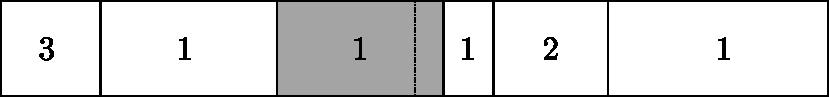
\includegraphics[width=.8\textwidth]{graphics/resnp.pdf}
    \end{center}
    \caption{
        \label{abb:resnp}
        Ein $2$-Bin mit $6$ Jobgruppen. Die Zahlen in den Jobgruppen geben an, wie viele Ressourcen für die Jobgruppe zur Verfügung stehen.
        Aktuell befindet sich eine Gruppe mit nur einer Ressource an der "`Bruchstelle"'.
        Durch Umordnung ist es evtl. möglich, dass eine der beiden Gruppen mit mehr als einer Ressource an diese Stelle gelangt.
    }
\end{figure}
\begin{satz}
    Das Problem zu entscheiden, ob die Jobgruppen in einem $k$-Bin (mit $k>1$) so angeordnet werden können,
    dass beim Zerlegen des $k$-Bins in $1$-Bins nur Jobgruppen mit mindestens zwei Ressourcen geteilt werden, ist $\mathcal{NP}$-vollständig.
\end{satz}
\begin{proof}
    Dieses Problem liegt trivialer Weise in $\mathcal{NP}$.
    Es muss also nur noch ein $\mathcal{NP}$-vollständiges Problem darauf reduziert werden.
    Es folgt die Reduktion des \textit{Partition}-Problems:
    Gegeben sei eine Instanz $J$ des \textit{Partition}-Problems mit Zahlen $a_1,\ldots,a_n$.
    Es sei $A\coloneqq\sum_{i=1}^{n}a_i$.
    Es wird eine Instanz $J'$ des gegebenen Problems erstellt mit $n+1$ Jobgruppen und einem $2$-Bin der Größe $A+2$.
    Es wird $g_i \coloneqq a_i$ für $1\leq i\leq n$ gesetzt und $g_{n+1}\coloneqq 2$.
    Für die Jobgruppen $1$ bis $n$ gibt es eine Ressource und für die Jobgruppe $n+1$ gibt es zwei Ressourcen.
    Die Jobgruppen müssen also so angeordnet werden, dass die Gruppe $n+1$ geteilt wird.
    Die resultierenden $1$-Bins haben dann jeweils die Größe $\frac{A}{2}+1$ und enthalten jeweils eine Jobgruppe der Größe $1$, die aus Gruppe $n+1$ hervorgehen.
    Wir zeigen: $J$ hat genau dann eine Lösung, wenn auch $J'$ eine hat.

    "`$\Rightarrow$"': $J$ habe eine Lösung, nämlich eine Teilmenge $T\subseteq\{1,\ldots,n\}$ mit $\sum_{i\in T}a_i = \frac{A}{2}$.
    Dann hat auch $J'$ eine Lösung: Alle $g\in T$ werden dem ersten $1$-Bin zugewiesen und alle $g\in\{1,\ldots,n\}\setminus T$ dem zweiten.
    In beiden $1$-Bins ist dann noch genau für eine Jobgruppe der Größe $1$ Platz, sodass jeweils eine Hälfte der Gruppe $n+1$ diesen ausfüllen kann.

    "`$\Leftarrow$"': Habe nun umgekehrt $J'$ eine Lösung. Da jeder $1$-Bin eine Jobgruppe der Größe $1$ enthält, die aus Gruppe $n+1$ hervorgegangen ist,
    müssen in beiden $1$-Bins die restlichen Jobgruppen zusammen jeweils die Größe $\frac{A}{2}$ haben.
    Diese Jobgruppen sind dann auch eine Lösung für $J$.
\end{proof}

In der Praxis kommt es allerdings selten vor, dass es nur eine Jobgruppe mit mehr als einer Ressource gibt.
Je mehr Jobgruppen mehr als eine Ressource haben, desto einfacher wird das Problem.
Der Fall, dass es keine Jobgruppe mit nur einer Ressource gibt ist trivial, da alle Jobgruppen ohne Bedenken geteilt werden können.

\subsubsection{Keine geeignete Anordnung möglich}
Es bleibt noch der Fall zu klären, dass in einem $k$-Bin keine geeignete Reihenfolge der Jobgruppen gefunden werden kann.
Es wird also mindestens eine Jobgruppe $g$ geteilt, obwohl es nur eine Ressource für sie gibt.

Zunächst kann versucht werden, das Binpacking und darauf aufbauend das Anordnen der Jobgruppen in den $k$-Bins zu wiederholen.
Evtl. besitzt eine Binpacking-Instanz mehrere Lösungen.
Dort werden dann ggf. andere Jobgruppen geteilt, so dass es evtl. keine möglichen Unzulässigkeiten mehr gibt.
Falls keine der Lösungen des Binpackings besser ist, kann die nächsten Zahlenpartition von $m$ getestet werden.
Je nachdem, ob in der nächsten Zahlenpartition $m'$ verringert wird (vgl. Abbildung \ref{abb:binpart}),
wird dadurch allerdings eine weitere Jobgruppenteilung und damit ein weiteres Mal Rüstkosten in Kauf genommen.

\begin{figure}
    \begin{center}
        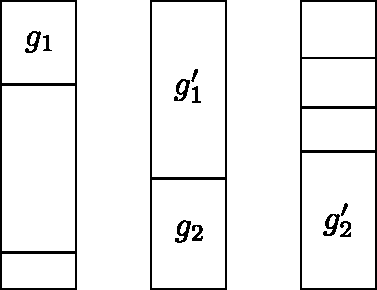
\includegraphics[width=.4\textwidth]{graphics/ueberlappen.pdf}
    \end{center}
    \caption{
        \label{abb:ueberlappen}
        Eine Instanz mit $m=3$ Bins, bei der die Jobgruppen $g$ und $g'$ geteilt wurden.
        Während es bei $g_1$ und $g_2$ immer möglich ist, sie so in ihren Bins anzuordnen, dass sie sich nicht überlappen
        (niemals gemeinsam in der Anlage sind), überlappen sich $g'_1$ und $g'_2$ zwangsweise immer.
    }
\end{figure}
Alternativ zum Anstieg der Rüstkosten können Bedingungen für die Nachfolgenden Verfahren, die $C_{\max}$ minimieren (s. Abschnitt \ref{sec:AnordnungDerJobgruppen}), 
formuliert werden:
Falls $n_g \leq \frac{n}{m}$ ist, ist es immer möglich, die beiden Teilgruppen, die aus $g$ hervorgehen,
so in den Bins anzuordnen, dass niemals zwei Jobs aus $g$ zur gleichen Zeit in der Anlage sind, indem beispielsweise
$g_1$ an den Anfang ihres Bins gelegt wird und $g_2$ ans Ende von ihrem Bin (vgl. Abbildung \ref{abb:ueberlappen}).
Falls mehrere Jobgruppen mit $n_g \leq \frac{n}{m}$ geteilt werden (es können höchstens $m-1$ sein), können in jedem Bin höchstens zwei resultierende 
Teilgruppen vorkommen, so dass es immer möglich ist, eine von beiden an den Anfang und die andere an das Ende des Bins zu legen.
Diese Bedingungen, dass die resultierenden Teilgruppen sich nicht \textit{überlappen} (vgl. Abbildung \ref{abb:ueberlappen}) dürfen, 
müssen dann in den nachfolgenden Verfahren beachtet werden.

Wenn $n_g > \frac{n}{m}$ ist,
gibt es keine Möglichkeit, $g$ so aufzuteilen, 
dass sich in jedem Zyklus höchstens ein Job aus $g$ in der Anlage befindet,
da nur $\frac{n}{m}$ Zyklen gemacht werden (vgl. Abbildung \ref{abb:ueberlappen}).
Da $g$ zu groß ist für einen Bin, muss $g$ aber zwangsweise irgendwo geteilt werden, so dass bei nur einer geeigneten Ressource definitiv keine zulässige Lösung existiert.
Dieser Umstand kann aber bereits im Voraus geprüft werden, so dass dieser Fall hier o.B.d.A. nicht auftritt.

\subsubsection{Zusammenfassung}
Insgesamt kann also nur sehr selten keine zulässige Ressourcenzuweisung gefunden werden.
Definitiv unzulässige Fälle sind häufig unabhängig von der Zuweisung der Jobgruppen an die Bins und können bereits im Voraus erkannt werden.
Da im Zweifelsfall sämtliche Lösungen von allen Zahlenpartitionen beim Binpacking durchprobiert werden, ist es ausgeschlossen, dass eine Lösung,
bei der nur solche Jobgruppen mit mehr als zwei Ressourcen geteilt werden, nicht gefunden wird, obwohl sie existiert.
Falls tatsächlich keine solche Lösung existiert, gibt es noch die Möglichkeit, in den nachfolgenden Verfahren mit zusätzlichen Nebenbedingungen darauf zu achten,
dass Teilgruppen sich nicht überlappen.


\section{Anordnung der Jobgruppen}
\label{sec:AnordnungDerJobgruppen}
In diesem Abschnitt werden Verfahren zur Anordnung der Jobgruppen in den Bins einerseits und
zum Zuordnen der Bins zu den Stationen andererseits vorgestellt.
Aus den vorangegangenen Verfahren (vgl. Abschnitt \ref{sec:Ressourcenzuweisung}) ist bekannt, zu welchen Bins die Jobgruppen gehören.
Geteilte Jobgruppen werden hier als eigenständige Gruppen betrachtet.
Auch eventuelle zusätzliche Restriktionen, dass die Teile einer geteilten Jobgruppe sich nicht überschneiden dürfen, sind bekannt.
Ziel ist es, $C_{\max}$ zu minimieren, ohne die Jobgruppen zu teilen und somit die bereits minimierten Rüstkosten zu verändern.

In Unterabschnitt \ref{subsec:MIPMitFixiertenBins} und \ref{subsec:MIPMitFreienBins} werden dazu zwei MIPs vorgestellt,
die allerdings der Einschränkung unterliegen, dass es nur zwei dominierende Maschinen geben darf.
Die in Unterabschnitt \ref{subsec:Nachbarschaftssuche} vorgestellte Nachbarschaftssuche hat diesbezüglich keine Einschränkungen.

\subsection{MIP mit fixierten Bins}
\label{subsec:MIPMitFixiertenBins}
Hier wird zunächst ein MIP vorgestellt, das lediglich die Jobgruppen in den Bins anordnet.
Die Bins sind dabei bereits fest den Stationen zugeordnet (der erste Bin zur ersten Station usw.).
Dieses MIP ist allerdings nur anwendbar bei zwei dominierenden Maschinen, die nicht notwendiger Weise benachbart sein müssen.
Ein MIP, das auch die Bins untereinander anordnet, d.h. den Stationen zuordnet, wird in Unterabschnitt \ref{subsec:MIPMitFreienBins} vorgestellt.

Die Idee des MIPs besteht darin, jeder Jobgruppe $i$ in ihrem Bin $b_i$ eine \textit{Startposition} $s_i$ zuzuweisen.
Aus der Startposition und der Länge $n_i$ einer Jobgruppe kann ihre \textit{Endposition} bestimmt werden.
Anhand dieser Start- und Endpositionen kann dann die Überlappung $o_{ij}$ mit einer anderen Jobgruppen $j$ aus einem anderen Bin $b_j$
berechnet werden.
Da die Bins den Stationen fest zugeordnet sind und es nur zwei dominierende Maschinen gibt, deren Abstand bekannt ist, 
müssen jeweils nur die Überlappungen von Jobs in Bins mit dem Abstand der dominierenden Maschinen berechnet werden.
Dazu ein Beispiel: Es gebe $m=8$ Maschinen, wobei $M_3$ und $M_4$ dominierend sind. 
Jobgruppe $1$ habe die Größe $n_1=10$ und liege im ersten Bin.
Jobgruppe $2$ habe die Größe $n_2=7$ und liege im zweiten Bin.
Da der Abstand der dominierenden Maschinen $1$ beträgt, wird der zweite Bin als \textit{Nachbarbin} von Bin 1 bezeichnet.
Bin 3 ist der Nachbarbin von Bin 2, Bin 4 ist der Nachbarbin von Bin 3, \ldots und Bin 1 ist der Nachbarbin von Bin 8.
Wenn der Abstand der dominierenden Maschinen hingegen z.B. $3$ betragen würde, dann wäre Bin 4 der Nachbarbin von Bin 1 usw.
Als erstes wird ein Job aus dem ersten Bin in die Anlage eingelegt, dann einer aus dem zweiten usw. 
Die Jobs im ersten Bin werden also immer genau in dem Moment von $M_4$ bearbeitet, wenn die Jobs im zweiten Bin von $M_3$ bearbeitet werden.
Die Startposition von Gruppe $1$ sei nun $s_1=0$ (als allererstes wird also ein Job aus Gruppe $1$ in die Anlage eingelegt)
und die Startposition von Gruppe $2$ sei $s_2=6$.
Die Überlappung der Gruppen $1$ und $2$ beträgt also $4$, wie auch in Abbildung \ref{abb:binfixbsp} zu sehen ist.
D.h. es kommt genau viermal vor, dass ein Job aus Gruppe $1$ von Maschine $M_4$ bearbeitet wird, während ein Job aus Gruppe $2$ von $M_3$ bearbeitet wird.
Da diese beiden Maschinen dominierend sind, beträgt die Zykluszeit in diesen vier Zyklen $\max\{p_{41},p_{32}\}$.
\begin{figure}
    \begin{center}
        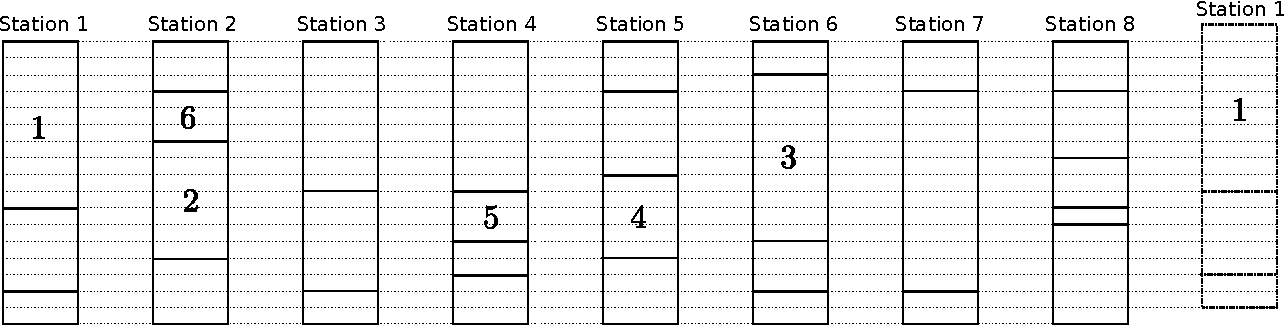
\includegraphics[width=\textwidth]{graphics/binfixbsp.pdf}
    \end{center}
    \caption{
        \label{abb:binfixbsp}
        Visualisierung einer Instanz mit $m=8$ Bins. 
        Rechts ist der Übergang von Station $8$ zu $1$ dargestellt, der um $1$ versetzt ist.
        Das liegt daran, dass nach dem $i$-ten Job im Bin auf Station $8$ der $i+1$-te Job im Bin auf Station $1$ folgt.
    }
\end{figure}

Ziel muss es also sein, den Jobgruppen Startpositionen in ihren Bins zuzuweisen und darauf basierend die Überlappungen mit Gruppen 
aus den Nachbarbins zu berechnen. 
Aus dem Maximum der Prozesszeiten der Jobgruppen und ihren Überlappungen kann dann $C_{\max}$ bestimmt werden.

Die Berechnung der Überlappungen $o_{ij}$ bildet den Kern dieses MIPs.
Es gibt fünf Möglichkeiten, wie sie berechnet werden müssen:
\begin{enumerate}
    \item $o_{ij} = s_i + n_i - s_j$, falls $s_i\leq s_j<s_i+n_i\leq s_j+n_j$ (z.B. $1$ und $2$ in Abb. \ref{abb:binfixbsp}),
    \item $o_{ij} = s_j + n_j - s_i$, falls $s_j\leq s_i<s_j+n_j\leq s_i+n_i$ (z.B. $3$ und $4$ in Abb. \ref{abb:binfixbsp}),
    \item $o_{ij} = n_i$, falls $s_j\leq s_i<s_i+n_i\leq s_j+n_j$ (z.B. $5$ und $4$ in Abb. \ref{abb:binfixbsp}),
    \item $o_{ij} = n_j$, falls $s_i\leq s_j<s_j+n_j\leq s_i+n_i$ (z.B. $1$ und $6$ in Abb. \ref{abb:binfixbsp}) und
    \item $o_{ij} = 0$, falls $s_i+n_i<s_j$ oder $s_j+n_j<s_i$.
\end{enumerate}
Dabei bezieht sich $i$ immer auf den Job im "`linken"' Bin und $j$ auf den im "`rechten"'.
Welche davon die passende ist, muss im MIP anhand einiger Hilfsvariablen und Nebenbedingung ermittelt werden.
Außerdem gibt es auch noch den Sonderfall, dass zwischen zwei Nachbarbins der Übergang von Station $m$ zu Station $1$ liegt.
Dieser Fall ist ebenfalls in Abbildung \ref{abb:binfixbsp} rechts veranschaulicht.
Wie dort zu sehen ist, muss dann die Berechnung der Überlappung leicht abgeändert werden, da Bin $1$ im Verhältnis zu Bin $m$ um 1 nach oben verschoben ist.
Die ersten beiden Möglichkeiten zur Berechnung der Überlappung ändern sich dann zu
\begin{enumerate}
    \item $o_{ij} = s_i + n_i + 1 - s_j$ und 
    \item $o_{ij} = s_j + n_j - s_i - 1$.
\end{enumerate}
Die Startpositionen von $i$ werden also jeweils um $1$ nach hinten verschoben, bzw. die von $j$ um $1$ nach vorn.
Zur Vereinfachung wird im MIP ein binärer Parameter $\sigma_{ij}$ benutzt, der genau dann den Wert $1$ hat, wenn dieser Sonderfall eintritt, und sonst $0$.
Auf diese Weise kann $\sigma_{ij}$ direkt in die Berechnung von $o_{ij}$ integriert werden:
\begin{enumerate}
    \item $o_{ij} = s_i + n_i + \sigma_{ij} - s_j$ und 
    \item $o_{ij} = s_j + n_j - s_i - \sigma_{ij}$.
\end{enumerate}

Um festzustellen, welche der Berechnungen für $o_{ij}$ benutzt werden muss, werden binäre Hilfsvariablen $y_{ij}$ und $z_{ij}$ verwendet.
Es ist $y_{ij}=1$ genau dann, wenn $s_j \geq s_i + \sigma_{ij}$ ist, d.h. $j$ "`startet"' gleichzeitig oder später als $i$.
Für $z_{ij}$ gilt in ähnlicher Weise: $z_{ij}=1$ genau dann, wenn $s_i + n_i + \sigma_{ij} \geq s_j + n_j$, 
d.h. die Endposition von $i$ liegt hinter der von $j$ oder gleichauf.
Aus den vier möglichen Kombinationen der Werte von $y_{ij}$ und $z_{ij}$ lässt sich bestimmen, 
welche der ersten vier Berechnungsmöglichkeiten für $o_{ij}$ gewählt werden muss.
Sollte diese Berechnung einen negativen Wert liefern, tritt der fünfte Fall ein.
Für die Jobs $1$ und $2$ in Abbildung \ref{abb:binfixbsp} wäre beispielsweise $y_{12}=1$ und $z_{12}=0$.

Im MIP wird mit $\tilde{N}=\{1,\ldots,\tilde{n}\}$ die Menge der Jobgruppen bezeichnet.
$B=\{1,\ldots,m\}$ ist die Menge der Bins und für $b\in B$ ist $\tilde{N}_b\subset \tilde{N}$ die Teilmenge der Jobgruppen, die in Bin $b$ liegen.
Für $i\in\tilde{N}$ gibt $b_i\in B$ den Bin an, in dem sich $i$ befindet.
$\tilde{N}_b^*\subset \tilde{N}$ bezeichnet die Menge der Jobgruppen im Nachbarbin von $b$.
$p_{1i}$ und $p_{2i}$ sind die Prozesszeiten von Jobgruppe $i$ auf der ersten bzw. zweiten dominierenden Maschine.
Für je zwei Jobgruppen $i,j\in N_b$, die im selben Bin $b$ liegen, gibt es
zwei Binärvariablen $x_{ij},x_{ji}$. Es ist $x_{ij}=1$ genau dann, wenn 
Jobgruppe $i$ vor $j$ in dem Bin liegt. Dabei muss $i$ nicht notwendiger
Weise direkt vor $j$ liegen, sondern an beliebiger Stelle davor.
Mithilfe der $x_{ij}$ lassen sich die Startpositionen $s_i$ bestimmen, mit denen wiederum die Überlappungen $o_{ij}$ wie oben beschrieben berechnet werden:
\begin{align}
    \text{min}\quad &\sum_{b\in B}\sum_{\substack{i\in \tilde{N_b}\\j\in \tilde{N}_b^*}} 
            \max\{p_{2i},p_{1j}\}o_{ij} \label{objfunc1}\\
			\text{s.t.} \quad x_{ij} + x_{ji} &= 1 &i\in \tilde{N}, j\in \tilde{N}_{b_i}, i<j \label{con1:reflex}\\
			x_{ij} + x_{jk} &\leq x_{ik} + 1 &i\in \tilde{N},\,\, j,k\in \tilde{N}_{b_i} \label{con1:transitiv} \\
			s_i &= \sum_{\substack{j\in \tilde{N}_{b_i}\\i\neq j}} n_j x_{ji} &i\in \tilde{N} \label{con1:start} \\
            My_{ij} &\geq s_j - s_i - \sigma_{ij} + \epsilon &i\in \tilde{N}, j\in \tilde{N}^*_{b_i} \label{con1:y1} \\
            M(1-y_{ij}) &\geq s_i - s_j + \sigma_{ij} &i\in \tilde{N}, j\in \tilde{N}^*_{b_i} \label{con1:y2} \\
            Mz_{ij} &\geq s_i + n_i - s_j - n_j + \sigma_{ij} + \epsilon &i\in \tilde{N}, j\in \tilde{N}^*_{b_i} \label{con1:z1} \\
            M(1-z_{ij}) &\geq s_j + n_j- s_i - n_i - \sigma_{ij} &i\in \tilde{N}, j\in \tilde{N}^*_{b_i} \label{con1:z2} \\
            o_{ij} &\geq s_i + n_i - s_j + \sigma_{ij} - M(1-y_{ij}+z_{ij}) &i\in \tilde{N}, j\in \tilde{N}^*_{b_i} \label{con1:o1} \\
            o_{ij} &\geq s_j + n_j - s_i - \sigma_{ij} - M(1-y_{ji}+z_{ji}) &i\in \tilde{N}, j\in \tilde{N}^*_{b_i} \label{con1:o2} \\
            o_{ij} &\geq n_j - M(2-y_{ij}-z_{ij}) &i\in \tilde{N}, j\in \tilde{N}^*_{b_i} \label{con1:o3} \\
            o_{ij} &\geq n_i - M(2-y_{ji}-z_{ji}) &i\in \tilde{N}, j\in \tilde{N}^*_{b_i} \label{con1:o4} \\
            o_{ij} &\geq 0 &i\in \tilde{N}, j\in \tilde{N}^*_{b_i} \label{con1:o5} \\
            x_{ij} &\in \{0,1\} &i\in \tilde{N}, j\in \tilde{N}_{b_i} \\
            y_{ij},z_{ij} &\in \{0,1\} &i\in \tilde{N}, j\in \tilde{N}^*_{b_i}
\end{align}
Mit (\ref{con1:reflex}) wird erreicht, dass immer entweder $i$ vor $j$ liegt
oder umgekehrt. (\ref{con1:transitiv}) stellt die Transitivität dieser Beziehung
her. Auf Grundlage der $x_{ij}$ und der Größen der Jobgruppen $n_i$ 
kann in (\ref{con1:start}) die Startposition jeder Jobgruppe berechnet werden.
Die Variablen $s_i$ dienen dabei nur der Übersicht und können in den übrigen 
Nebenbedingungen durch die Summe aus (\ref{con1:start}) ersetzt werden.
Über (\ref{con1:y1}) und (\ref{con1:y2}) wird den Indikatorvariablen $y_{ij}$ 
mit einem "`Big-M"' die oben beschriebene Bedeutung gegeben:
(\ref{con1:y1}) setzt $y_{ij}$ auf $1$, wenn $s_j-s_i-\sigma_{ij}+\epsilon > 0$ ist,
was äquivalent zu $s_j \geq s_i+\sigma_{ij}$ ist.
$\epsilon$ ist ein hinreichend kleiner Parameter, falls alle Prozesszeiten ganzzahlig sind, ist jeder Wert $\epsilon<1$ geeignet.
(\ref{con1:y2}) andererseits setzt $y_{ij}$ auf $0$, wenn $s_i-s_j+\sigma_{ij} > 0$ ist (oder äquivalent dazu: $s_j < s_i+\sigma_{ij}$).
Analog wird mit (\ref{con1:z1}) und (\ref{con1:z2}) der Wert der $z_{ij}$ entsprechend der obigen Bedeutung gesetzt.
Je nachdem, welche der $y_{ij}$ und $z_{ij}$ auf $1$ bzw. $0$ gesetzt sind, 
werden drei der vier Nebenbedingungen (\ref{con1:o1}) bis (\ref{con1:o4}) durch die "`Big-Ms"' faktisch bedeutungslos ($o_{ij}\geq \text{"`ein negativer Wert"'}$)
und nur eine bleibt bestehen, so dass genau die passende der vier Berechnungsmöglichkeiten für die $o_{ij}$ gewählt wird.
Für $y_{ij}=1$ und $z_{ij}=0$, wie bei den Jobs $1$ und $2$ in Abbildung \ref{abb:binfixbsp} der Fall, 
würde beispielsweise das "`Big-M"' aus (\ref{con1:o1}) verschwinden, so dass die Bedingung $o_{ij}\geq s_i+n_i-s_j$ "`übrigbleibt"'.
Da die Zielfunktion (\ref{objfunc1}) die Überlappungen (mit dem Maximum der jeweiligen Prozesszeiten multipliziert) minimiert,
wird daraus de facto $o_{ij}=s_i+n_i-s_j$ und die $o_{ij}$ müssen auch nicht per Nebenbedingung nach oben beschränkt werden.
Sie sind automatisch durch die Größe der Bins beschränkt.
Damit sie nicht negativ werden, sind sie allerdings durch (\ref{con1:o5}) nach unten durch $0$ beschränkt.
Dies bedeutet, dass die jeweiligen Jobgruppen sich nicht überschneiden.

Die Qualität der Lösung dieses MIPs ist stark von der gegebenen Zuordnung der Bins an die Stationen abhängig.
Bei einigen Zuordnungen kann es sehr gute Lösungen geben, und bei anderen dagegen nur sehr schlechte, was sich nur durch eine
Änderung der Zuordnung (bzw. der Binreihenfolge) verbessern lässt, wozu dieses MIP allerdings nicht in der Lage ist.
Im Folgenden wird daher ein weiteres MIP vorgestellt, das diese Fähigkeit besitzt, und heuristische Methoden,
die die Bins den Stationen zuweisen, um darauf basierend dieses MIP anzuwenden.


\subsection{MIP mit freien Bins}
\label{subsec:MIPMitFreienBins}
Das folgende MIP erweitert das MIP aus Unterabschnitt \ref{subsec:MIPMitFixiertenBins} um die Fähigkeit, die Bins untereinander zu vertauschen,
was dem Zuweisen der Bins an die Stationen entspricht.
Für die Berechnung der Überschneidungen zwischen den Jobgruppen sind daher weitere Variablen notwendig, die als Indikator dafür dienen,
ob die Bins der Jobgruppen auf benachbarten Stationen liegen.
Dazu dienen die Binärvariablen $\beta_{bd}$, die genau dann auf $1$ gesetzt werden, wenn Bin $b$ Station $d$ zugewiesen ist.
Weitere Binärvariablen $\nu_{bcd}$ werden auf $1$ gesetzt, wenn Bin $b$ Station $d$ zugewiesen ist und Bin $c$ der Nachbarstation von $d$ (mit $d^*$ bezeichnet).
Auf diese Weise können die $\nu_{bcd}$ die $\sigma_{ij}$ aus dem MIP in Unterabschnitt \ref{subsec:MIPMitFixiertenBins} ersetzen:
Wenn die beiden dominierenden Maschinen benachbart sind (also den Abstand $1$ haben), ist für zwei Jobgruppen $i$ und $j$ $\nu_{b_ib_jm}=1$ genau dann, 
wenn der Bin von $i$ der letzten Station $m$ zugewiesen ist und der Bin von $j$ der ersten Station (also genau dann, wenn im anderen MIP $\sigma_{ij}=1$ ist).
Außerdem gibt es weitere Binärvariablen $w_{ij}$, die als Indikator dafür dienen, ob die Bins der Jobgruppen $i$ und $j$ benachbarten Stationen zugewiesen sind.
Denn nur dann muss zwischen diesen Jobgruppen die Überlappung $o_{ij}$ berechnet werden.
\begin{align}
    \text{min}\quad &\sum_{\substack{i,j\in\tilde{N}\\b_i\neq b_j}} 
            \max\{p_{2i},p_{1j}\}o_{ij} \label{objfunc}\\
    \text{s.t.} \quad x_{ij} + x_{ji} &= 1 &i\in\tilde{N}, j\in\tilde{N}_{b_i} 
            \label{con:reflex}\\
    x_{ij} + x_{jk} &\leq x_{ik} + 1 &i\in\tilde{N},\,\, j,k\in\tilde{N}_{b_i} 
            \label{con:transitiv} \\
    s_i &= \sum_{\substack{j\in\tilde{N}_{b_i}\\i\neq j}} g_j x_{ji} &i\in\tilde{N} 
            \label{con:start} \\
	\sum_{b\in B}\beta_{bd} &= 1 &d\in B \label{con:binpos} \\
	\sum_{d\in B}\beta_{bd} &= 1 &b\in B \label{con:binpos2} \\
	\beta_{bd} + \beta_{cd^*} &\leq \nu_{bcd} + 1 &b,c,d\in B \label{con:nu} \\
	\nu_{bcd} &\leq \beta_{bd} &b,c,d\in B \label{con:nurev} \\
    \nu_{bcd} &\leq \beta_{bd^*} &b,c,d\in B \label{con:nurev2} \\
    My_{ij} &\geq s_j - s_i - \nu_{b_ib_jm} + \epsilon &i,j\in\tilde{N} \label{con:y1}\\
    M(1-y_{ij}) &\geq s_i + \nu_{b_ib_jm} - s_j &i,j\in\tilde{N} \\
    Mz_{ij} &\geq s_i + n_i + \nu_{b_ib_jm} - s_j - n_j + \epsilon &i,j\in\tilde{N} \\
    M(1-z_{ij}) &\geq s_j + n_j - s_i - n_i - \nu_{b_ib_jm} &i,j\in\tilde{N} \\
	w_{ij} &= \sum_{d\in B} \nu_{b_ib_jd} &i,j\in\tilde{N} \label{con:w} \\
    o_{ij} &\geq s_i + n_i + \nu_{b_ib_jm} - s_j \notag \\
		   &\phantom{\geq} - M(2-y_{ij}+z_{ij}-w_{ij}) &i,j\in\tilde{N} \label{con:o1} \\
    o_{ij} &\geq s_j + n_j - s_i - \nu_{b_ib_jm} \notag \\
           &\phantom{\geq} - M(2+y_{ij}-z_{ij}-w_{ij}) &i,j\in\tilde{N} \label{con:o2} \\
    o_{ij} &\geq n_j - M(3-y_{ij}-z_{ij}-w_{ij}) &i,j\in\tilde{N} \\
	o_{ij} &\geq n_i - M(1+y_{ij}+z_{ij}-w_{ij}) &i,j\in\tilde{N} \label{con:o4} \\
    o_{ij} &\geq 0 &i,j\in\tilde{N} \\
	\beta_{bd} &\in \{0,1\} &b,d\in B \\
	\nu_{bcd} &\in \{0,1\} &b,c,d\in B, b\neq c \\
    x_{ij} &\in \{0,1\} &i\in\tilde{N},j\in\tilde{N}_{b_i} \\
    y_{ij},z_{ij},w_{ij} &\in \{0,1\} &i,j\in\tilde{N}
\end{align}
Die Nebenbedingungen (\ref{con:binpos}) und (\ref{con:binpos2}) gewährleisten, dass jeder der $m$ Bins genau einer der $m$ Stationen zugewiesen wird.
Über die Nebenbedingungen (\ref{con:nu}), (\ref{con:nurev}) und (\ref{con:nurev2}) wird erzwungen, dass die Binärvariablen
$\nu_{bcd}$ genau dann auf $1$ gesetzt werden, wenn Bin $b$ Station $d$ zugewiesen ist und zugleich Bin $c$ der Nachbarstation $d^*$.
In (\ref{con:w}) wird $w_{ij}$ auf $1$ gesetzt, falls die Bins von $i$ und $j$ benachbarten Stationen zugewiesen sind.
Wenn $w_{ij}=0$ ist, verlieren die Nebenbedingungen (\ref{con:o1}) bis (\ref{con:o4}) ihre Bedeutung.
Davon abgesehen sind diese Nebenbedingungen aber identisch zu denen aus dem MIP im vorherigen Unterabschnitt.
Ähnlich wie die $s_i$ dienen die $w_{ij}$ nur der Übersicht und können durch die Summe in (\ref{con:w}) ersetzt werden.

In dieser Form verlangt das MIP, dass die beiden dominierenden Maschinen benachbart sein müssen.
Denn dann gibt es nur zwei Stationen, zwischen denen die Berechnung der Überlappung um $1$ versetzt stattfinden muss.
Wenn die dominierenden Maschinen beispielsweise einen Abstand von $2$ haben,
tritt dieser Sonderfall der Berechnung sowohl zwischen den Station $m-1$ und $1$ auf als auch zwischen $m$ und $2$,
was durch die Variablen $\nu_{b_i,b_j,m-1}$ bzw. $\nu_{b_ib_jm}$ erkannt werden kann.
Diese müssten dann auch beide in die Nebenbedingungen (\ref{con:y1}) bis (\ref{con:o2}) einfließen.
Da immer höchstens eine von beiden gleichzeitig auf $1$ gesetzt sein kann, 
bewirken dann diese beiden Variablen zusammen die um $1$ versetzte Berechnung der Überlappung.
Nebenbedingung (\ref{con:y1}) z.B. sähe dann so aus:
\[ My_{ij} \geq s_j - s_i - \nu_{b_ib_jm} - \nu_{b_i,b_j,m-1} + \epsilon \quad i,j\in\tilde{N} \]

Das Lösen dieses MIPs mit CPLEX dauert sehr viel länger als beim MIP mit fixierten Bins.
Allerdings ist die obere Schranke, also die aktuell beste gefundene Lösung, meist schon nach wenigen Minuten besser als die
beste Lösung mit fixierten Bins (abhängig davon, ob die gegebene Binreihenfolge dort zufällig "`gut"' ist).

\subsection{Mehrere fixierte Reihenfolgen}
Das MIP in Unterabschnitt \ref{subsec:MIPMitFreienBins} liefert zwar theoretisch optimale Lösungen, diese zu berechnen benötigt aber zu viel Zeit.
Schon bei kleinen Instanzen mit $\tilde{n}=10$ Jobgruppen und $m=8$ beträgt der LP-Gap nach einer Stunde Berechnung noch $20\%$.
Man beachte, dass es bei $10$ Jobgruppen und $8$ Bins mindestens $6$ Bins gibt mit genau einer Jobgruppe.
Es müssen also im Wesentlichen nur noch die Bins den Stationen zugeordnet werden und trotzdem ist die Laufzeit so lang.

Das MIP mit fixierten Bins hingegen findet erst ab Instanzen mit ca. $\tilde{n}=25$ nicht mehr die optimale Lösung innerhalb von einer Stunde.
Je nach Größe der Jobgruppen kann dies ein beträchtlicher Unterschied zu $\tilde{n}=10$ sein. 
Allerdings ist die Güte der Lösungen des MIPs mit fixierten Bins von der initialen Binreihenfolge abhängig.
Dazu wird in diesem Unterabschnitt versucht, solch eine initiale Binreihenfolge zu erzeugen, mit der das MIP dann arbeiten kann.

\subsubsection{Benutzung beider MIPs}
Beobachtungen der Leistung der beiden MIPs haben ergeben, dass das MIP mit freien Bins oft schon nach relativ kurzer Zeit eine bessere obere Schranke
(d.h. die beste bis zu diesem Zeitpunkt gefundene Lösung) liefert als das MIP mit fixierten Bins.
Daher ist ein Ansatz, das MIP mit freien Bins für eine gewisse Zeit laufen zu lassen und dann die Zuteilung der Bins zu den Stationen
auszulesen (diese ist in den $\beta_{bd}$-Variablen kodiert), um anschließend mit dieser Binreihenfolge das MIP mit fixierten Bins zu starten.
%hier noch ein bisschen mehr schreiben...


\subsubsection{Optimum zwischen zwei Bins}
Betrachtet man zwei beliebige Bins $a$ und $b$ auf benachbarten Stationen, ist es möglich, 
all jene Zyklen $t$ zu betrachten, in denen ein Job aus $a$ auf der zweiten dominierenden Maschine ist und ein Job aus $b$ auf der ersten.
Die zugehörigen Zykluszeiten $c_t$ werden dann durch die Prozesszeiten dieser Jobs auf den beiden dominierenden Maschinen definiert.%evtl ein Bild?
Die Summe dieser Zykluszeiten zwischen zwei benachbarten Bins $a$ und $b$ wird mit $C_{ab}$ bezeichnet.
\begin{satz}
    Seien $a$ und $b$ zwei Bins auf benachbarten Stationen.
    Wenn die Jobgruppen in $a$ absteigend nach ihren Prozesszeiten auf der zweiten dominierenden Maschine angeordnet werden
    und die Jobgruppen in $b$ absteigend nach ihren Prozesszeiten auf der ersten dominierenden Maschine,
    dann ist $C_{ab}$ minimal.
\end{satz}
\begin{proof}
    Für den Beweis werden nicht die Jobgruppen, sondern die einzelnen Jobs betrachtet, was aber für die zu betrachtende Sortierung keinen Unterschied macht.
    Sei $C_{ab}^*$ die Summe der Zykluszeiten zwischen $a$ und $b$, wenn diese wie gefordert sortiert sind.
    Wir nehmen an, es gäbe eine andere Anordnung der Jobs mit $C_{ab} < C_{ab}^*$ und führen dies zu einem Widerspruch.
    Da die gegeben Sortierung in der anderen Anordnung nicht vorliegt, muss es dort in $a$ oder $b$ zwei benachbarte Jobs entgegen dieser Sortierung geben.
    Seien $j_1^a$ und $j_2^a$ diese Jobs und o.B.d.A. seien sie in Bin $a$.
    Die Jobs die an gleicher Position in Bin $b$ sind, werden mit $j_1^b$ und $j_2^b$ bezeichnet.
    Falls auch $j_1^b$ und $j_2^b$ entgegen dieser Sortierung angeordnet sind, 
    vertauschen wir sowohl $j_1^a$ mit $j_2^a$ als auch $j_1^b$ mit $j_2^b$ und ändern dadurch $C_{ab}$ nicht.
    Insbesondere hat sich $C_{ab}$ nicht verschlechtert, dadurch, dass wir uns der gewünschten Reihenfolge der Jobs in den Bins annähern.

    Andernfalls, wenn $j_1^b$ und $j_2^b$ bereits in der gewünschten Reihenfolge sind,
    verwenden wir zur besseren Lesbarkeit die Abkürzungen 
    $p_{1a}\coloneqq p_{2j_1^a}, p_{2a}\coloneqq p_{2j_2^a}, p_{1b}\coloneqq p_{1j_1^b}$ und $p_{2b}\coloneqq p_{1j_2^b}$.
    Es gilt also nach Annahme $p_{1a} < p_{2a}$ und $p_{1b}\geq p_{2b}$.
    Die entsprechenden beiden Zykluszeiten werden über $c_{t_1}=\max\{p_{1a},p_{1b}\}$ und $c_{t_2}=\max\{p_{2a},p_{2b}\}$ berechnet.
    Werden nun $j_1^a$ und $j_2^a$ vertauscht, ändert sich der Wert von $C_{ab}$ zu
    \[ C'_{ab} = C_{ab} - \max\{p_{1a},p_{1b}\} - \max\{p_{2a},p_{2b}\} + \max\{p_{2a},p_{1b}\} + \max\{p_{1a},p_{2b}\} \text{.}\]
    Wir betrachten nun zwei Fälle:
    \begin{enumerate}
        \item $p_{1a}\geq p_{1b}$: Es ist dann $p_{2b}\leq p_{1b}\leq p_{1a} < p_{2a}$ und somit
            \[ C'_{ab} = C_{ab} - p_{1a} - p_{2a} + p_{2a} + p_{1a} = C_{ab} \text{.} \]
            $C_{ab}$ verschlechtert sich in diesem Fall also nicht.
        \item $p_{1a} < p_{1b}$: In diesem Fall unterscheiden wir wieder zwei Fälle:
            \begin{enumerate}
                \item $p_{2a}\leq p_{2b}$: Es ist dann $p_{1a} < p_{2a}\leq p_{2b}\leq p_{1b}$ und somit
                    \[ C'_{ab} = C_{ab} - p_{1b} - p_{2b} + p_{1b} + p_{2b} = C_{ab} \text{.} \]
                    $C_{ab}$ verschlechtert sich in diesem Fall also ebenfalls nicht.
                \item $p_{2a} > p_{2b}$: Es ist dann $p_{1b},p_{2a} \geq p_{1a},p_{2b}$ und somit
                \begin{align}
                C'_{ab} &= C_{ab} - p_{1b} - p_{2a} + \max\{p_{2a},p_{1b}\} + \max\{p_{1a},p_{2b}\} \notag \\
                        &= C_{ab} - \min\{p_{1b},p_{2a}\} + \max\{p_{1a},p_{2b}\} \notag \\
                        &\leq C_{ab} \text{.} \notag
                \end{align}
                Also verschlechtert sich $C_{ab}$ auch hier nicht.
            \end{enumerate}
    \end{enumerate}
    Insgesamt verschlechtert sich $C_{ab}$ also niemals, während die Jobs in den Bins absteigend nach ihren Prozesszeiten sortiert werden.
    Das ist ein Widerspruch zu der Annahme, dass die ursprüngliche Anordnung besser war als die sortierte ($C_{ab} < C_{ab}^*$).
\end{proof}
Wie auch schon im Beweis geschehen, wird die Bezeichnung $C_{ab}^*$ für ein minimales $C_{ab}^*$ verwendet.
Dieses Optimum zwischen zwei Bins ist auf die Anordnung aller $m$ Bins übertragen aber nur ein lokales:
Wird ein Bin bezüglich eines seiner Nachbarn in dieser Weise angeordnet, ist es im Allgemeinen nicht der Fall,
dass diese Anordnung auch bezüglich des anderen Nachbarn optimal ist.

In den folgenden Absätzen werden einige Anwendungen dieses lokalen Optimierens vorgestellt.

\subsubsection{Bestimmung einer unteren Schranke}
\label{subsubsec:BestimmungEinerUnterenSchranke}
Eine Anwendungsmöglichkeit der lokal optimalen Bins ist die Berechnung einer unteren Schranke für die Summe der Zykluszeiten im zweiten Dekompositionsansatz.
Eine mögliche untere Schranke lässt sich wie folgt berechnen:
\[LB_{\sum c_t} = \frac{1}{2} \sum_{b=1}^m \left( \min_{a\neq b} C_{ab}^* + \min_{c\neq b} C_{bc}^* \right) \]
Es werden also für jeden Bin $b$ sein optimaler linker Nachbar $a$ und sein optimaler rechter Nachbar $c$ gesucht.
Da in der Summe all dieser $C_{ab}^*$-Werte jeder Bin zweimal (einmal als linker und einmal als rechter Nachbar) auftaucht,
wird diese Summe noch halbiert.
Zusammen mit den auftretenden Rüstkosten, die nach der Zuweisung der Jobgruppen an die Bins feststehen (vgl. Abschnitt \ref{sec:Ressourcenzuweisung}),
ist dies eine untere Schranke für die Zielfunktion $C_{\max}$.

\subsubsection{Heuristik für initiale Binreihenfolge}
\label{subsubsec:HeuristikFuerInitialeBinreihenfolge}
Eine andere mögliche Anwendung der lokal optimalen Bins ist, eine initiale Binreihenfolge (bzw. eine initiale Zuweisung der Bins zu den Stationen)
auf heuristischem Wege zu finden, mit der dann das MIP mit fixierten Bins arbeiten kann.
Als erster Schritt wird unter allen möglichen $C_{ab}^*$-Werten (für alle Bins $a,b$) das Minimum gesucht.
Die zugehörigen Bins $a$ und $b$ werden der ersten Station und der Nachbarstation der ersten Station zugewiesen.
Anschließend wird unter allen noch nicht zugewiesenen Bins derjenige Bin $c$ gesucht, der den besten $C_{bc}^*$-Wert aufweist.
Da $c$ ein "`vielversprechender"' Nachbar für $b$ ist, wird er der Nachbarstation von $b$ zugewiesen.
Dieses Vorgehen wird so lange wiederholt, bis jeder Bin einer Station zugewiesen ist.

Falls der Abstand der dominierenden Maschinen $d_{\mathit{dom}}$($=$Abstand benachbarter Stationen) und die Anzahl der Maschinen $m$ nicht teilerfremd sind,
gibt es unter den Stationen disjunkte Gruppen, die untereinander nicht durch Nachbarschaft erreicht werden können.
Beispielsweise bilden bei $m=8$ und $d_{\mathit{dom}}=2$ die Stationen $1,3,5,7$ und $2,4,6,8$ solche disjunkten Gruppen.
In diesem Fall muss das obige Verfahren für jede dieser Gruppen separat durchgeführt werden.

\subsubsection{Heuristik zum Anordnen der Jobgruppen in den Bins}
\label{subsubsec:HzAdJidB}
Die lokal optimalen Bins können auch benutzt werden, um auf heuristischem Wege die Jobgruppen in den Bins bei gegebener Binreihenfolge anzuordnen.
Dazu werden jeweils vier direkt benachbarte Bins $a,b,c,d$ gesucht ($a$ ist linker Nachbar von $b$, $b$ ist linker Nachbar von $c$ und $c$ ist linker Nachbar von $d$).
Seien $C_{ab},C_{bc}$ und $C_{cd}$ die aktuellen Summen der Zykluszeiten zwischen diesen Bins.
Nun werden die Jobgruppen in $b$ und $c$ so sortiert, dass $C_{bc}=C_{bc}^*$ wird.
Dadurch ändern sich auch die Zykluszeiten zwischen $a$ und $b$ zu $C'_{ab}$ und die zwischen $c$ und $d$ zu $C'_{cd}$.
Wenn $C'_{ab}+C_{bc}^*+C'_{cd} < C_{ab}+C_{bc}+C_{cd}$ ist, wird die Änderung übernommen, andernfalls verworfen.
Dieses Vorgehen wird so lange wiederholt, bis keine benachbarten Bins $a,b,c,d$ mehr gefunden werden, die auf diese Weise optimiert werden können.


\subsection{Nachbarschaftssuche}
\label{subsec:Nachbarschaftssuche}
Als Alternative zu den MIPs mit freien oder fixierten Bins lassen sich Nachbarschaftsoperatoren beschreiben, 
die für diverse Nachbarschaftssuchverfahren benutzt werden können.
Naheliegende Operatoren sind:
\begin{itemize}
    \item $\mathit{bch}_{bc}$: vertauscht die Bins an den Stationen $b$ und $c$ miteinander,
    \item $\mathit{jch}_{bjk}$: vertauscht im Bin an Station $b$ die Jobgruppen $j$ und $k$ miteinander.
\end{itemize}
Es wurde ein Simulated Annealing Algorithmus implementiert, der diese beiden Nachbarschaften benutzt.
Dieser ähnelt dem Simulated Annealing aus Abschnitt \ref{subsubsec:Nachbarschaftssuche} und unterscheidet sich bloß in einem Punkt von diesem:
In jeder Iteration wird mit einer Wahrscheinlichkeit von $\frac{m}{\tilde{n}+m}$ eine neue Lösung aus der $\mathit{bch}_{bc}$-Nachbarschaft erzeugt 
(mit zufällig gewählten $b$ und $c$) und mit einer Wahrscheinlichkeit von $\frac{\tilde{n}}{\tilde{n}+m}$ eine Lösung aus der $\mathit{jch}_{bjk}$-Nachbarschaft
(mit ebenfalls zufälligen $b,j,k$).
Auf diese Weise wird je nach Verhältnis zwischen der Anzahl der Jobgruppen ($\tilde{n}$) und der Bins ($m$) der entsprechende Operator häufiger benutzt.

Im Gegensatz zu den beiden MIPs sind Lösungsansätze, die auf diesen Nachbarschaftsoperatoren basieren, nicht darauf angewiesen, 
dass nur zwei Maschinen dominierend sind. Ebenso müssen die Rüstkosten nicht konstant sein, wie von den MIPs verlangt, sondern können beliebig sein.


\section{Algorithmenvarianten}
\label{sec:Algorithmenvarianten}
Im ersten Abschnitt dieses Kapitels (\ref{sec:Ressourcenzuweisung}) wurde ein Verfahren vorgestellt, 
das die Jobgruppen $m$ Bins zuordnet und im Fall der Teilung einer Jobgruppe auf Zulässigkeit achtet,
um so die minimale Anzahl an Rüstkosten zu verursachen.
Dieser Schritt ist essenziell für den zweiten Dekompositionsansatz, da sämtliche Verfahren, die im zweiten Abschnitt \ref{sec:AnordnungDerJobgruppen} vorgestellt wurden,
auf dieser Zuordnung operieren und sie nachträglich nicht mehr ändern.
Da die Verfahren in Abschnitt \ref{sec:AnordnungDerJobgruppen} aber sehr vielfältig sind, 
werden hier noch einmal alle Varianten der Zuordnung der Bins an die Stationen und der Anordnung der Jobgruppen in den Bins zusammengefasst:
\begin{enumerate}
    \item Wende ausschließlich das MIP mit fixierten Bins an für eine Zeit $t$.%\textit{Güte der Lösung hängt stark von der initialen Zuweisung der Bins an die Stationen ab.}
    \item Wende das MIP mit freien Bins für eine Zeit $t_1$ an und lese die bis dahin berechnete Zuordnung der Bins an die Stationen aus.
        Wende das MIP mit fixierten Bins mit dieser Zuordnung für eine Zeit $t_2$ an.
    \item Wende die Heuristik für eine initiale Binreihenfolge (\ref{subsubsec:HeuristikFuerInitialeBinreihenfolge}) an.
        Wende das MIP mit fixierten Bins mit dieser Zuordnung für eine Zeit $t$ an.
    \item Wende das MIP mit freien Bins für eine Zeit $t$ an und lese die bis dahin berechnete Zuordnung der Bins an die Stationen aus.
        Wende die Heuristik zum Anordnen der Jobgruppen in den Bins (\ref{subsubsec:HzAdJidB}) an auf diese Zuordnung an.
    \item Wende die Heuristik für eine initiale Binreihenfolge (\ref{subsubsec:HeuristikFuerInitialeBinreihenfolge}) an.
        Wende die Heuristik zum Anordnen der Jobgruppen in den Bins (\ref{subsubsec:HzAdJidB}) an auf diese Zuordnung an.
    \item Wende den Simulated-Annealing-Ansatz (\ref{subsec:Nachbarschaftssuche}) an.
\end{enumerate}
Bis auf das Simulated-Annealing bestehen alle Ansätze aus zwei Stufen: 
In der ersten Stufe werden die Bins untereinander angeordnet und in der zweiten Stufe werden die Jobgruppen in den Bins angeordnet.
Diese Ansätze werden in Kapitel \ref{chap:RechenergebnisseUndVergleiche} evaluiert.



\chapter{Rechenergebnisse und Vergleiche}
\label{chap:RechenergebnisseUndVergleiche}
In diesem Kapitel werden Rechenergebnisse vorgestellt und miteinander verglichen.
Es wurden sowohl selbst generierte Instanzen getestet als auch solche aus der Praxis eines Küchenherstellers.
Getestet wurde auf einem PC mit Intel(R) Xeon(R) CPU E3-1230 v3, 8 Kerne @ 3.30GHz, und 16GB RAM unter Ubuntu 13.10.
Die MIPs wurden mit ZIMPL \cite{Koch2004} und CPLEX v12.6 gelöst.
Die übrigen Algorithmen wurden in C++ implementiert und mit dem GCC v4.8.1 mit O2-Optimierung kompiliert.

In Abschnitt \ref{subsec:VergleichDerHeuristiken} werden die in Abschnitt \ref{subsec:HeuristischeVerfahren} vorgestellten Heuristiken evaluiert
und mit drei Heuristiken verglichen, die Soylu et al. in ihrem Paper \cite{soylu} präsentieren.
In Abschnitt \ref{sec:VergleichDerDekompositionsansaetze} werden die beiden Dekompositionsansätze miteinander verglichen.


\section{Vergleich der Heuristiken}
\label{subsec:VergleichDerHeuristiken}
In diesem Abschnitt werden die Rechenergebnisse der Heuristiken aus Unterabschnitt \ref{subsec:HeuristischeVerfahren} vorgestellt und miteinander verglichen.
Es wurden vier eigene Testreihen mit zufälligen Instanzen erzeugt und auch eine Testreihe wie in \cite{soylu} beschrieben. 

\subsection{Eigene Testinstanzen}
Die vier hier vorgestellten Testreihen haben folgende Parameter: 
\begin{itemize}
    \item $m=8$ Maschinen und 
    \item $n=50,100,150,\ldots,5000$ Jobs.
\end{itemize}
In der ersten Testreihe sind die Maschinen $M_3,M_4,M_5$ dominierend.
Ihre Prozesszeiten wurden gleichverteilt aus dem Intervall $[10,100]$ gewählt.
Die Prozesszeiten der übrigen Maschinen wurden aus dem Intervall $[0,9]$ gleichverteilt gewählt.
In Abbildung \ref{abb:3dom} sind die Resultate aufgetragen.
\begin{figure}
    \begin{center}
        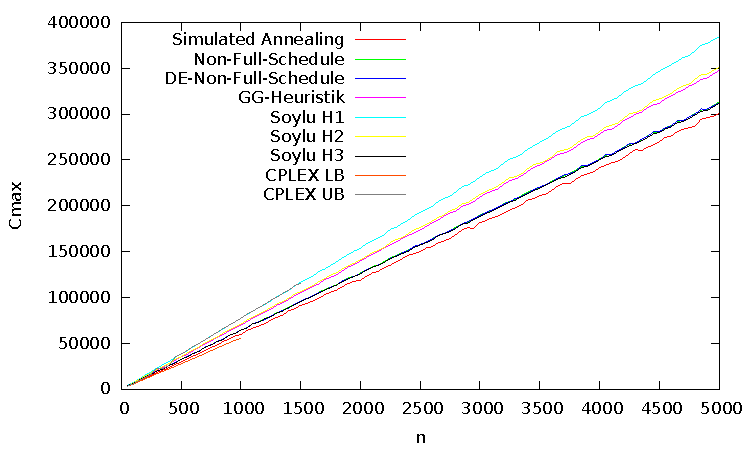
\includegraphics[width=.8\textwidth]{../instances/3dom/plot.pdf}
    \end{center}
    \begin{center}
        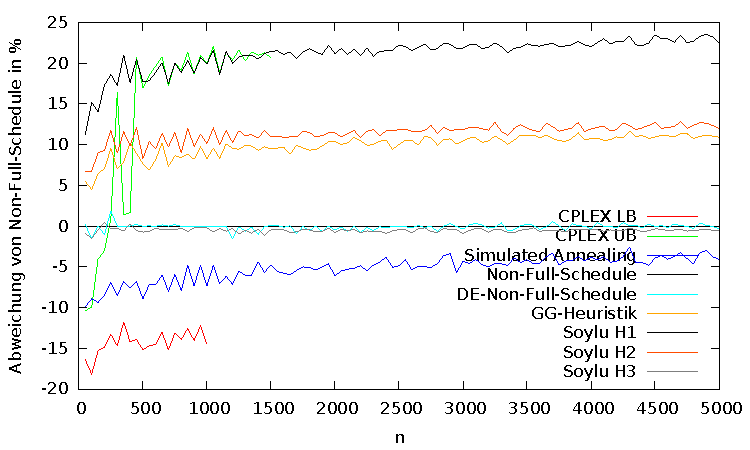
\includegraphics[width=.8\textwidth]{../instances/3dom/plotrel.pdf}
    \end{center}
    \caption{
        \label{abb:3dom}
        Resultate der Heuristiken für die Summe der Zykluszeiten (oben) 
        und relative Unterschiede zwischen der Non-Full-Schedule-Heuristik und den übrigen Heuristiken (unten) 
        bei drei dominierenden Maschinen (gleichverteilte Prozesszeiten).
    }
\end{figure}
Oben sind die Summe der Zykluszeiten in Abhängigkeit von der Instanzgröße $n$ aufgetragen.
Da die Resultate sehr ähnlich sind, so dass die Kurven teilweise sehr dicht beieinander liegen, 
sind unten jeweils die relativen Differenzen $\frac{C_{\max,h}-C_{\max,nfs}}{C_{\max,nfs}}$ der übrigen Heuristiken ($h$) zur Non-Full-Schedule-Heuristik ($nfs$) aufgetragen.
CPLEX LB und UB bezeichnen die untere und obere Schranke, die CPLEX nach 30 Minuten errechnet hat.
Dabei ist die obere Schranke der Zielfunktionswert einer tatsächlich errechneten Lösung und kann daher als Heuristik verwendet werden.
Zu sehen ist, dass die Lösungen des MIPs bei sehr kleinen Instanzen ($n<300$) nach einer halben Stunde Rechenzeit vergleichbar mit den Lösungen der übrigen Heuristiken sind.
Allerdings benutzt CPLEX alle 8 Prozessorkerne parallel, während die übrigen Heuristiken nicht parallel implementiert sind.
Außerdem liegen die Rechenzeiten der übrigen Heuristiken weit unter einer halben Stunde (s. Abbildung \ref{abb:3domtime}).
Aus diesen Gründen wurde das MIP auch nur bis zu Instanzgrößen von $n=1500$ berechnet.
\begin{figure}
    \begin{center}
        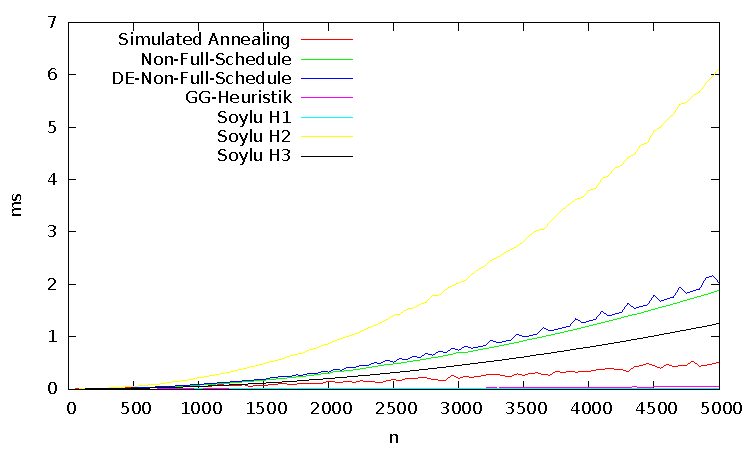
\includegraphics[width=.8\textwidth]{../instances/3dom/plottime.pdf}
    \end{center}
    \caption{
        \label{abb:3domtime}
        Laufzeiten der drei Heuristiken bei drei dominierenden Maschinen (gleichverteilte Prozesszeiten).
    }
\end{figure}

Außerdem ist zu erkennen, dass die Double Ended Non-Full-Schedule-Heuristik fast identische Resultate liefert im Vergleich zur Non-Full-Schedule-Heuristik.
$H_3$ von Soylu ist meist etwas besser als als diese beiden.
Die Gilmore-Gomory-Heuristik liefert hier relativ schlechte Resultate.
Schlechter sind nur $H_2$ von Soylu und mit einigem Abstand $H_3$.
Mit Simulated Annealing konnten hier offenbar die besten Lösungen erzeugt werden.
Der Plot der relativen Abweichungen zeigt außerdem, dass diese Abweichungen offenbar nahezu konstant sind zwischen den Heuristiken (nicht beim MIP) 
und nicht von der Instanzgröße abhängen.
Einzig die relative Abweichung des Simulated Annealings scheint mit zunehmender Instanzgröße leicht abzunehmen.

In Abbildung \ref{abb:3domtime} sind die Zeiten aufgetragen, die die Heuristiken benötigten, um die in Abbildung \ref{abb:3dom} dargestellten Resultate zu berechnen.
Deutlich zu erkennen ist der quadratische Anstieg der beiden Non-Full-Schedule-Heuristiken und Soylus $H_3$, wobei die Double Ended Variante etwas langsamer ist,
da pro Iteration immer zwei Jobs statt nur einem gesucht werden, und $H_3$ etwas schneller, da kein zweites Vergleichskriterium angewandt wird.
Außerdem treten in der Kurve der Double Ended Non-Full-Schedule-Heuristik teilweise kleine Ausreißer nach oben auf.
Eine plausible Begründung hierfür konnte nicht gefunden werden.
Die Kurve des Simulated Annealings ist, wie zu erwarten war, sehr chaotisch, was durch die nicht deterministische Funktionsweise des Algorithmus erklärt werden kann:
Die Laufzeit hängt stark vom Zufall ab und nur zweitrangig von der Instanzgröße.
Am schnellsten sind die Gilmore-Gomory-Heuristik und $H_1$, die dafür aber beide vergleichsweise schlechte Resultate liefern.
$H_2$ hingegen ist mit Abstand am langsamsten trotz der eher schlechten Resultate.

Die zweite Testreihe unterscheidet sich nur dadurch von der ersten, dass die Prozesszeiten der dominierenden Maschinen nicht gleichverteilt aus dem Intervall
$[10,100]$ ausgewählt wurden, sondern normalverteilt mit einem Erwartungswert von $\mu=50$ und einer Standardabweichung von $\sigma=20$.
Die Resultate sind analog zur ersten Testreihe in Abbildung \ref{abb:3domnorm} dargestellt und die Laufzeiten dazu in Abbildung \ref{abb:3domnormtime}.
\begin{figure}
    \begin{center}
        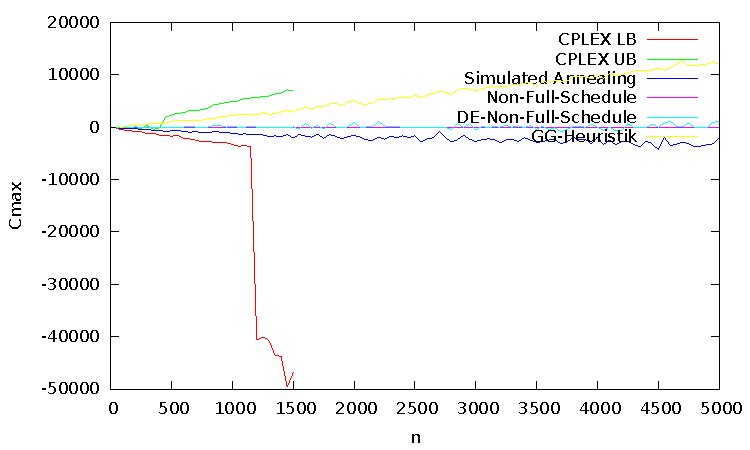
\includegraphics[width=.8\textwidth]{../instances/3dom_norm/plot.pdf}
    \end{center}
    \begin{center}
        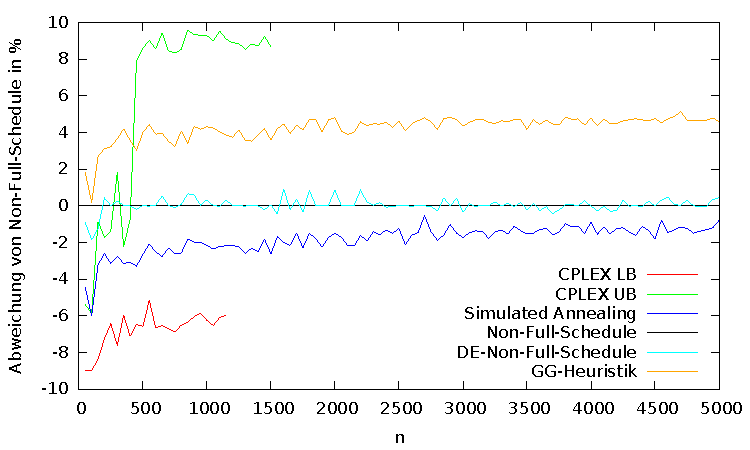
\includegraphics[width=.8\textwidth]{../instances/3dom_norm/plotrel.pdf}
    \end{center}
    \caption{
        \label{abb:3domnorm}
        Resultate der Heuristiken für die Summe der Zykluszeiten (oben) 
        und relative Unterschiede zwischen der Non-Full-Schedule-Heuristik und den übrigen Heuristiken (unten) 
        bei drei dominierenden Maschinen (normalverteilte Prozesszeiten).
    }
\end{figure}
\begin{figure}
    \begin{center}
        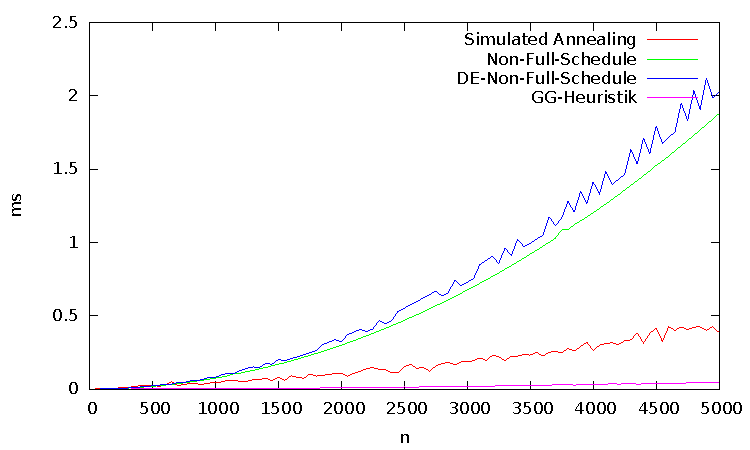
\includegraphics[width=.8\textwidth]{../instances/3dom_norm/plottime.pdf}
    \end{center}
    \caption{
        \label{abb:3domnormtime}
        Laufzeiten der drei Heuristiken bei drei dominierenden Maschinen (normalverteilte Prozesszeiten).
    }
\end{figure}

Die Laufzeiten der zweiten Testreihe unterscheiden sich nur marginal von denen der ersten, was zu erwarten war, 
da die Laufzeiten der Heuristiken nicht von den Prozesszeiten abhängig sind.
Die Kurven in Abbildung \ref{abb:3domnorm} unterscheiden sich im Verlauf kaum von denen in Abbildung \ref{abb:3dom}.
Allerdings sind diese Kurven im Vergleich zur ersten Testreihe in etwa um den Faktor $2$ gestaucht.
Die Resultate der Heuristiken unterscheiden sich hier also weniger.
Das muss daran liegen, dass die Prozesszeiten (da sie normalverteilt sind) weniger unterschiedlich sind.
Die beiden Non-Full-Schedule-Heuristiken, $H_2$ und $H_3$ ziehen daraus einen Vorteil, da sie nach eben diesem Prinzip vorgehen, möglichst ähnliche Prozesszeiten zu finden.
Auch die Gilmore-Gomory-Heuristik profitiert davon, da beim (theoretischen) Wiederhochskalieren der Prozesszeiten der dritten dominierenden Maschine 
nur vergleichsweise wenige Zykluszeiten mit vergrößert werden müssen.
Auch CPLEX kommt bei diesen Daten offenbar ebenfalls schneller zu besseren Schranken.
Selbst $H_1$ liefert bessere Ergebnisse, obwohl die Jobs hier im Wesentlichen (bis auf $m$ Jobs) zufällig angeordnet sind.
Durch die Normalverteilung ist es selbst bei zufälligen Reihenfolgen wahrscheinlich, dass in einem Zyklus ähnliche Prozesszeiten sind.


Die dritte Testreihe wurde mit einem identischen Verfahren wie die zweite Testreihe generiert.
Allerdings wurde der Erwartungswert der Prozesszeiten auf Maschine $M_3$ auf $\mu=30$ festgesetzt, also um $20$ weniger gegenüber $M_4$ und $M_5$.
Ziel sollte es sein, dass $M_4$ und $M_5$ nicht dominierend sind, sondern nur eine geringe Semidominanz haben, 
so dass die Vorzüge der Gilmore-Gomory-Heuristik zum Tragen kommen.
\begin{figure}
    \begin{center}
        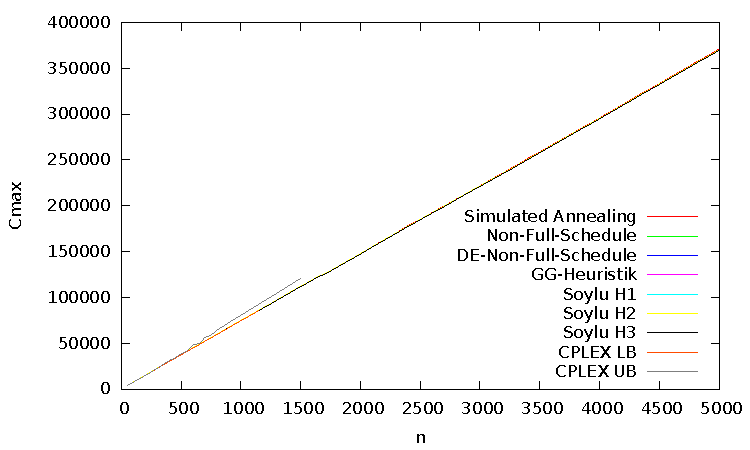
\includegraphics[width=.8\textwidth]{../instances/2quasidom/plot.pdf}
    \end{center}
    \begin{center}
        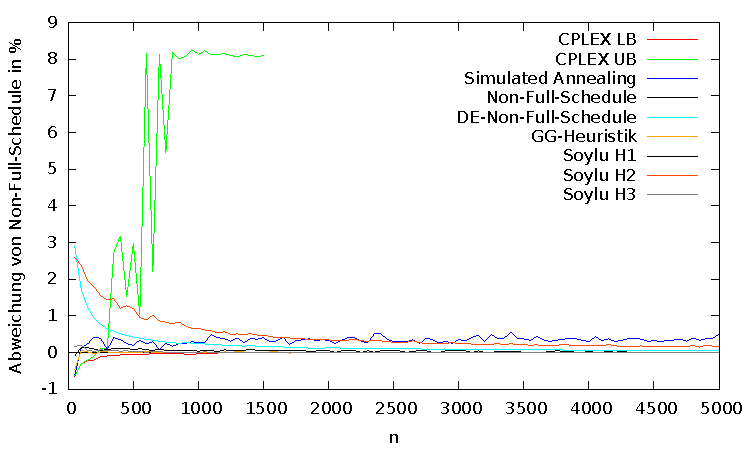
\includegraphics[width=.8\textwidth]{../instances/2quasidom/plotrel.pdf}
    \end{center}
    \caption{
        \label{abb:2quasidom}
        Resultate der Heuristiken für die Summe der Zykluszeiten (oben) 
        und relative Unterschiede zwischen der Non-Full-Schedule-Heuristik und den übrigen Heuristiken (unten) 
        bei zwei semidominierenden Maschinen (normalverteilte Prozesszeiten).
    }
\end{figure}
\begin{figure}
    \begin{center}
        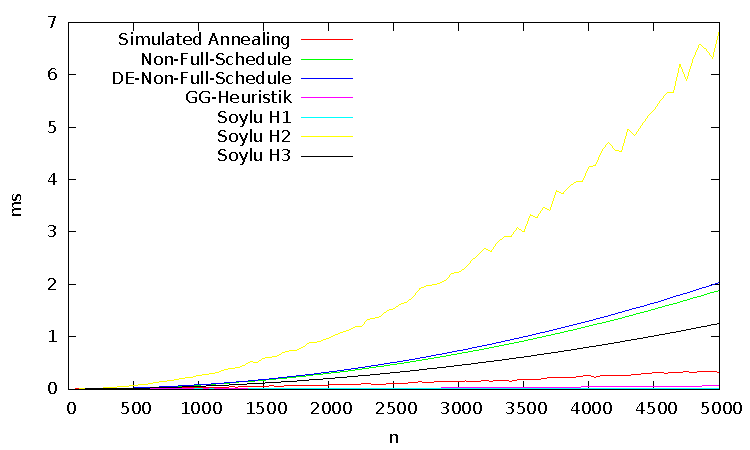
\includegraphics[width=.8\textwidth]{../instances/2quasidom/plottime.pdf}
    \end{center}
    \caption{
        \label{abb:2quasidomtime}
        Laufzeiten der drei Heuristiken bei zwei semidominierenden Maschinen (normalverteilte Prozesszeiten).
    }
\end{figure}

Und tatsächlich bestätigen die Rechenergebnisse diese Vermutung, wie in Abbildung \ref{abb:2quasidom} zu sehen ist.
Fast alle Heuristiken liefern bessere Ergebnisse als sie es bei den ersten beiden Testreihen tun (in der gleichen Zeit, s. Abbildung \ref{abb:2quasidomtime}).
Simulated Annealing ist hier allerdings nicht mehr die beste Heuristik.
Die besten Resultate liefern hier die Gilmore-Gomory-Heuristik, die die größte Verbesserung gegenüber den anderen Testreihen erfährt, 
und die Non-Full-Schedule-Heuristik. Die Resultate von beiden sind nahezu identisch.
Die Double Ended Non-Full-Schedule-Heuristik ist hier bei allen Instanzen schlechter als die Non-Full-Schedule-Heuristik, wenn auch nur um weniger als $1\%$
bzw. bis zu $3\%$ bei sehr kleinen Instanzen.
Bemerkenswert ist außerdem, dass die untere Schranke, die von CPLEX für Instanzen mit $n\leq 1500$ berechnet wurde,
oft bis an die Ergebnisse der Gilmore-Gomory- und der Non-Full-Schedule-Heuristik heranreicht.
Das bedeutet, dass die Resultate dieser beiden Heuristiken nahezu optimal sind.
Andererseits sind die oberen Schranken von CPLEX vergleichsweise weit von den Resultaten der Heuristiken entfernt.
%Als Ausblick könnten diese Heuristiken daher in CPLEX integriert werden, um die oberen Schranken zu verbessern.

Die vierte Testreihe wurde genau wie die erste generiert, allerdings mit nur zwei dominierenden Maschinen $M_3$ und $M_4$.
Da in diesem Fall die Gilmore-Gomory-Heuristik ein optimales Ergebnis liefert, wurde das MIP nicht auf diese Instanzen angewandt.
Ziel dieser Testreihe ist es, die Güte der Heuristiken anhand eines optimalen Vergleichswertes bestimmen zu können.
\begin{figure}
    \begin{center}
        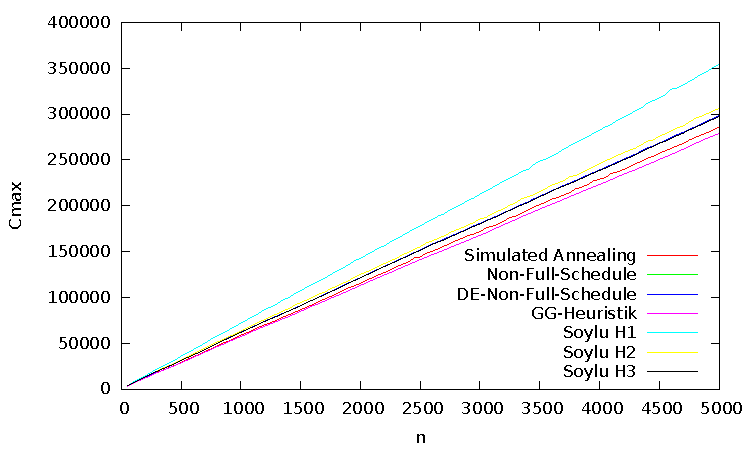
\includegraphics[width=.8\textwidth]{../instances/2dom/plot.pdf}
    \end{center}
    \begin{center}
        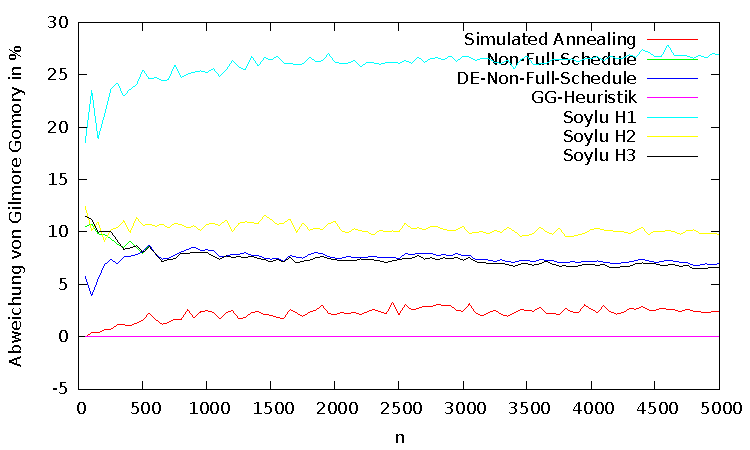
\includegraphics[width=.8\textwidth]{../instances/2dom/plotrel.pdf}
    \end{center}
    \caption{
        \label{abb:2dom}
        Resultate der Heuristiken für die Summe der Zykluszeiten (oben) 
        und relative Unterschiede zwischen der Gilmore-Gomory-Heuristik und den übrigen Heuristiken (unten) 
        bei zwei dominierenden Maschinen (gleichverteilte Prozesszeiten).
    }
\end{figure}
In Abbildung \ref{abb:2dom} sind analog zu den anderen Testreihen die Ergebnisse aufgetragen.
Wie zu sehen ist, liefert Simulated Annealing (abgesehen von Gilmore Gomory) die besten Ergebnisse mit nur etwa $2{,}5\%$ Abweichung vom Optimum.
Danach folgen fast gleich auf die beiden Non-Full-Schedule-Heuristiken und $H_3$.
Bei vielen Instanzen liefern $H_3$ und die Non-Full-Schedule-Heuristik sogar identische Resultate, 
während die Double Ended Non-Full-Schedule-Heuristik minimal schlechter ist.
Bis Instanzgrößen von $n=500$ ist sie allerdings besser als die anderen beiden.
Weit abgeschlagen sind $H_1$ und $H_2$.
Da die einzelnen Heuristiken unterschiedlich viel Nutzen aus dem Umstand ziehen, dass es zwei benachbarte dominierende Maschinen gibt,
sind die Resultate dieser Testreihe allerdings nur bedingt auf andere Instanzen mit mehr als zwei dominierenden Maschinen übertragbar.

\subsection{Instanzen von Soylu et al.}
In ihrem Paper \cite{soylu} generieren Soylu et al. ebenfalls einige Instanzen, mit denen sie ihre Heuristiken testen.
Da diese mit $n\leq 50$ eine sehr viel kleinere Größe haben als die bislang hier getesteten Instanzen, 
ist es sinnvoll einige davon im Rahmen dieser Arbeit zu generieren und die Heuristiken auch mit anhand dieser zu evaluieren.
Es wurden Instanzen mit $n=20,25,30,35$ Jobs generiert, die auf $\tilde{n}=2,3,\ldots,\frac{n}{5}$ Jobgruppen aufgeteilt sind.
Dabei hat jeweils eine Jobgruppe die Größe $n_g=\frac{n}{2}$ und die übrigen Jobs werden gleichmäßig auf die anderen Jobgruppen aufgeteilt.
Es gibt $m=2,3,4$ Maschinen und die Prozesszeiten $p_{ij}$ werden gleichverteilt aus dem Intervall $[1,10]$ gewählt.
In den Abbildungen \ref{abb:soylutest2}, \ref{abb:soylutest3} und \ref{abb:soylutest4} sind die Resultate aller Heuristiken für diese Instanzen aufgetragen.
An der Beschriftung der horizontalen Achse können die Eigenschaften der Instanz abgelesen werden.
Dabei ist $r$ Bezeichnung von Soylu et al. für die Anzahl der Jobgruppen ($\tilde{n}$).

\begin{figure}
    \begin{center}
        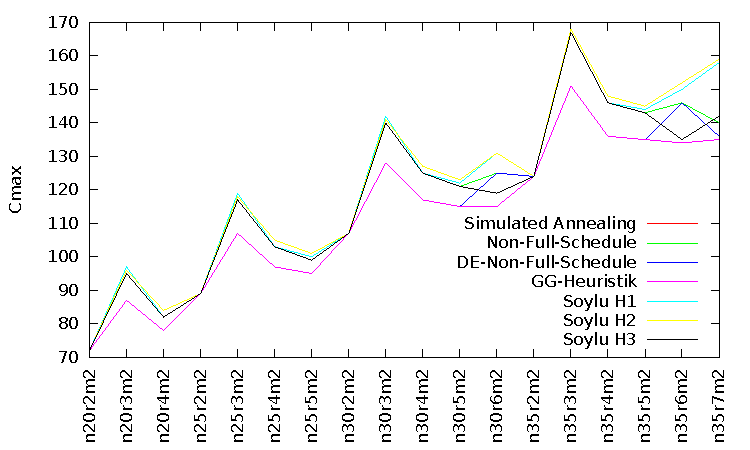
\includegraphics[width=.8\textwidth]{../instances/soylu/plotm2.pdf}
    \end{center}
    \caption{
        \label{abb:soylutest2}
        Resultate der Heuristiken auf den Instanzen von Soylu et al. mit $m=2$.
    }
\end{figure}
Für $m=2$ ist in Abbildung \ref{abb:soylutest2} zu sehen, dass Simulated Annealing immer die optimale Lösung gefunden hat, was daran zu erkennen ist,
dass die Kurven für Simulated Annealing und Gilmore Gomory sich vollständig überlagern (Gilmore Gomory ist bei $m=2$ optimal).
Alle übrigen Heuristiken liefern stehts sehr ähnliche Ergebnisse, wobei häufig $H_1$ oder $H_2$ am schlechtesten ist.
Interessant ist, dass jeweils bei Instanzen mit $r=\tilde{n}=2$ alle Heuristiken eine optimale Lösung finden.
Das kann dadurch erklärt werden, dass es bei zwei Maschinen und zwei Jobgruppen nicht viele sich wesentlich unterscheidende Möglichkeiten gibt, diese anzuordnen.

\begin{figure}
    \begin{center}
        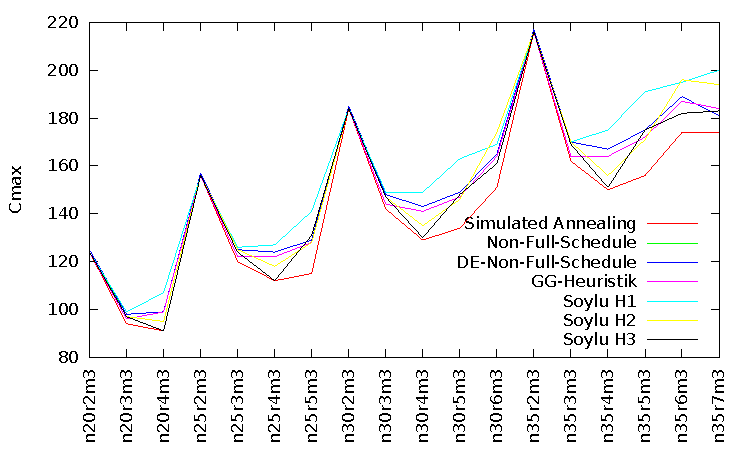
\includegraphics[width=.8\textwidth]{../instances/soylu/plotm3.pdf}
    \end{center}
    \caption{
        \label{abb:soylutest3}
        Resultate der Heuristiken auf den Instanzen von Soylu et al. mit $m=3$.
    }
\end{figure}
Auch bei Instanzen mit $m=3$ in Abbildung \ref{abb:soylutest3} liefern alle Heuristiken bei $r=\tilde{n}=2$ die gleichen Resultate.
Wie auch bei $m=2$ liefert Simulated Annealing immer die besten Lösungen.
Es kann allerdings nicht überprüft werden, ob diese optimal sind, da die Gilmore-Gomory-Heuristik hier keine optimalen Vergleichswerte liefern kann.
Da aber diese Instanzen mit $n\leq 35$ genauso klein sind wie die in Abbildung \ref{abb:soylutest2}, kann vermutet werden,
dass die Ergebnisse des Simulated Annealings auch hier nahezu optimal sind.
$H_1$ und $H_2$ schneiden auch hier häufig sehr schlecht ab. 
$H_3$ hingegen liefert bei Instanzen mit $r=\tilde{n}=4$ die zweitbeste Lösung und ist dort besser als die beiden Non-Full-Schedule-Heuristiken 
(diese liefern fast immer das gleiche Ergebnis, weshalb sich die Graphen überlagern und kaum zu unterscheiden sind)
obwohl diese nach einem ähnlichen Prinzip arbeiten.

\begin{figure}
    \begin{center}
        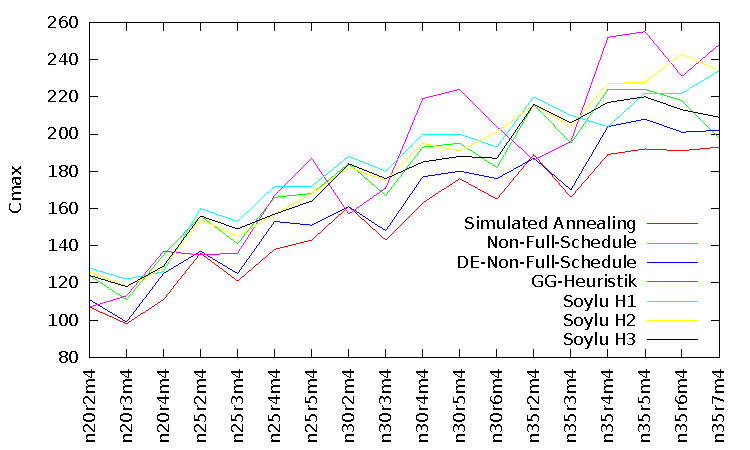
\includegraphics[width=.8\textwidth]{../instances/soylu/plotm4.pdf}
    \end{center}
    \caption{
        \label{abb:soylutest4}
        Resultate der Heuristiken auf den Instanzen von Soylu et al. mit $m=4$.
    }
\end{figure}
Bei Instanzen mit $m=4$ (s. Abbildung \ref{abb:soylutest4}) liefern alle Heuristiken deutlich verschiedene Ergebnisse.
Bis auf drei Ausnahmen bei $r=\tilde{n}=2$ ist wieder Simulated Annealing am besten.
Oft schneidet hier die Gilmore-Gomory-Heuristik besonders schlecht ab, da sie bei wenigen dominierenden Maschinen am besten ist.
Besonders gute Resultate liefert hier neben Simulated Annealing die Double Ended Non-Full-Schedule-Heuristik und ist im Gegensatz zu den Instanzen mit $m=2$ und $m=3$ nicht 
fast identisch mit der Non-Full-Schedule-Heuristik und $H_3$.

\subsection{Zusammenfassung}
Unter allen Heuristiken ist Simulated Annealing oft am besten, während $H_1$ und $H_2$ von Soylu et al. oft sehr schlecht abschneiden.
Das gilt sowohl für die selbst generierten Instanzen als auch für die von Soylu et al.
Die Gilmore-Gomory-Heuristik liefert nur dann gute Ergebnisse, wenn zwei benachbarte Maschinen dominierend sind (dann sind die Ergebnisse optimal)
oder semidominant. Sind diese Voraussetzungen nicht gegeben, sind auch keine guten Ergebnisse von der Gilmore-Gomory-Heuristik zu erwarten.
Die Double Ended Non-Full-Schedule-Heuristik, die Non-Full-Schedule-Heuristik und $H_3$ von Soylu et al. gehen sehr ähnlich vor, 
was sich auch in ihren Resultaten widerspiegelt.
Für jede der drei gibt es Instanzen, bei denen sie besser sind als die anderen beiden, so dass nur schwer vorausgesagt werden kann, welche wann am besten ist.

\section{Vergleich der Dekompositionsansätze}
\label{sec:VergleichDerDekompositionsansaetze} 
In diesem Abschnitt werden die beiden Dekompositionsansätze aus den Kapiteln \ref{chap:DerErsteDekompositionsansatz} und \ref{chap:DerZweiteDekompositionsansatz}
miteinander verglichen. Ziel ist es, eine Aussage darüber zu treffen, in welchen Situationen welcher Ansatz die besseren Ergebnisse liefert.
Da der zweite Dekompositionsansatz sich weitestgehend auf den Fall beschränkt, dass es zwei dominierende Maschinen gibt,
Rüstkosten konstant sind ($s_{fg}=s$) und die Ressourcenmengen der Jobgruppen disjunkt sind, werden hier auch nur solche Instanzen betrachtet.
Außerdem liegt diese Situation auch bei dem betrachteten Praxisfall des Küchenherstellers vor, der einige reale Instanzen zur Verfügung gestellt hat.

Im Fall von zwei benachbarten dominierenden Maschinen liefert der Algorithmus von Gilmore und Gomory eine optimale Lösung für den ersten Schritt des ersten
Dekompositionsansatzes, das Erstellen einer Jobreihenfolge $\pi$ ohne die Ressourcen und Rüstkosten zu berücksichtigen.
Da danach noch der zweite Schritt folgt, in dem $\pi$ auf Zulässigkeit bezüglich verfügbarer Ressourcen überprüft wird
und ggf. nachträglich noch geändert wird, ist es trotzdem sinnvoll, auch die Heuristiken aus Abschnitt \ref{subsec:HeuristischeVerfahren} anzuwenden.

In den folgenden Unterabschnitten werden zwei Testreihen betrachtet: In \ref{subsec:RealeInstanzen} werden Instanzen betrachtet, 
die von dem Küchenhersteller zur Verfügung gestellt wurden und daher direkten Praxisbezug haben.
In Unterabschnitt \ref{subsec:GenerierteInstanzen} werden zufällig erzeugte Instanzen betrachtet.

\subsection{Reale Instanzen}
\label{subsec:RealeInstanzen}
Die hier betrachteten Instanzen stammen aus einer realen Anwendung.
Die Instanzen haben eine Größe von 37-68 Jobgruppen, wobei jede Jobgruppe zwischen 1 und 1400 Jobs umfasst. Besonders große Jobgruppen sind dabei selten.
Die meisten Jobgruppen bestehen aus weniger als 100 Jobs.
Die Zeit für einen Ressourcenwechsel beträgt $s_{fg}=s=5$.
Es gibt $m=8$ Maschinen, von denen zwei benachbarte dominierend sind.
Die Prozesszeiten auf den dominierenden Maschinen liegen zwischen $0{,}5$ und $2$ Minuten und für jede Jobgruppe gibt es zwischen 1 und 15 geeignete Ressourcen.
Da es sich bei einer der beiden Maschinen in diesem Praxisfall um eine menschliche Arbeitskraft handelt, 
durften die Prozesszeiten dieser "`Maschine"' nicht herausgegeben werden.
Daher ist für beide Maschinen jeweils die gleiche Prozesszeit angegeben.
Um dies auszugleichen, wurde für jede Jobgruppe die Prozesszeit einer zufälligen Maschine um einen zufälligen Wert zwischen $0$ und $0{,}5$ Minuten verringert.
Die Daten sind also nicht mehr zu $100\%$ original.

\subsubsection{Resultate des ersten Dekompositionsansatzes}
\label{subsubsec:ResultateDKA1}
Zunächst soll der erste Dekompositionsansatz betrachtet werden.
Dabei werden erst die unterschiedlichen Heuristiken angewandt und anschließend wird $\pi$ wie in Abschnitt \label{sec:UnzulaessigeReihenfolgen} beschrieben korrigiert.
In Abbildung \ref{abb:kbheurplot} ist zu sehen, wie gut der von den Heuristiken erzeugte (noch nicht korrigierte) Wert für $C_{\max}$ in Abhängigkeit von $n$ ist.
Gilmore-Gomory liefert die optimale Lösung, die Lösungen von Simulated Annealing sind nahezu optimal und am schlechtesten schneidet $H_1$ ab.
\begin{figure}
    \begin{center}
        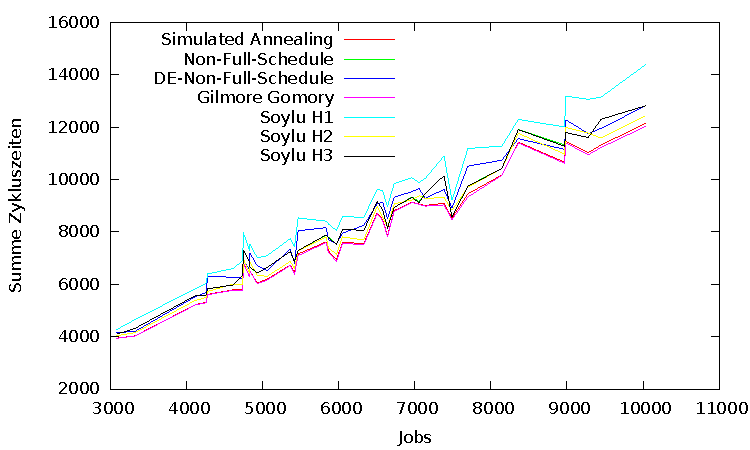
\includegraphics[width=.8\textwidth]{../prog/heuristics/plots/kbheurplot.pdf}
    \end{center}
    \caption{
        \label{abb:kbheurplot}
        Summe der Zykluszeiten, wenn $\pi$ mit der jeweiligen Heuristik erzeugt wurde.
    }
\end{figure}

In Abbildung \ref{abb:kbplot} sind die Summen der Zykluszeiten aufgetragen, \textit{nachdem} $\pi$ korrigiert worden ist.
Falls das Resultat einer Heuristik nicht so abgewandelt werden konnte, dass eine gültige Ressourcenzuweisung möglich ist, 
ist an der entsprechenden Stelle in der Kurve eine Lücke gelassen.
\begin{figure}
    \begin{center}
        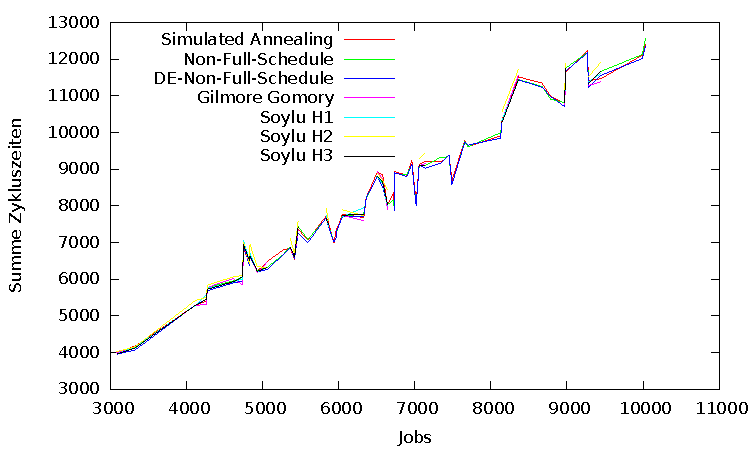
\includegraphics[width=.8\textwidth]{../prog/heuristics/plots/kbplot.pdf}
    \end{center}
    \caption{
        \label{abb:kbplot}
        Summe der Zykluszeiten, nachdem $\pi$ mit der jeweiligen Heuristik erzeugt und anschließend ggf. korrigiert wurde.
    }
\end{figure}
Wie zu sehen ist, sind die Resultate der Heuristiken nach der Korrektur nahezu identisch, obwohl die Heuristiken teilweise von sehr unterschiedlicher Güte sind
(s. Abbildung \ref{abb:kbheurplot}).
Allerdings treten einige Lücken in den Kurven auf, also nicht korrigierbare Ergebnisse (durch die Nähe der Kurven schwer zu erkennen).
Zum Vergleich sind in Abbildung \ref{abb:kbdiffplot} die Differenzen aufgetragen zwischen den Resultaten nach und vor der Korrektur.
\begin{figure}
    \begin{center}
        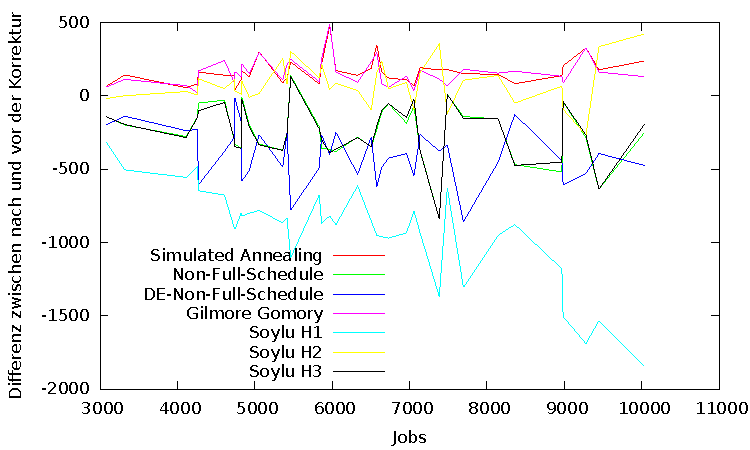
\includegraphics[width=.8\textwidth]{../prog/heuristics/plots/kbdiffplot.pdf}
    \end{center}
    \caption{
        \label{abb:kbdiffplot}
        Differenzen zwischen den Resultaten nach und vor der Korrektur.
    }
\end{figure}
Wie dort zu erkennen ist, werden die Resultate vieler Heuristiken durch die Korrektur nicht verschlechtert, sondern teils sogar erheblich verbessert.
Dieses Phänomen tritt vor allem bei den Heuristiken auf, deren Resultate vorher eher schlecht waren. 
Das kann dadurch erklärt werden, dass bei der Korrektur im Falle der Wahlmöglichkeit immer solche Jobs getauscht werden,
durch die die Summe der Zykluszeiten möglichst wenig verschlechtert -- oder eben sogar verbessert -- wird.
Das wiederum bedeutet, dass bei den Ergebnissen der jeweiligen Heuristiken (auch ohne Ressourcen und Rüstkosten zu betrachten)
teils noch enormes Verbesserungspotential besteht, das allein durch Iterative Improvement mit einer Vertausch-Nachbarschaft abgerufen werden kann.

In Abbildung \ref{abb:kbcoplot} sind die zugehörigen Rüstkosten aufgetragen, die nach der Korrektur noch in $\pi$ auftreten.
Lücken bedeuten wieder, dass keine Korrektur möglich war.
\begin{figure}
    \begin{center}
        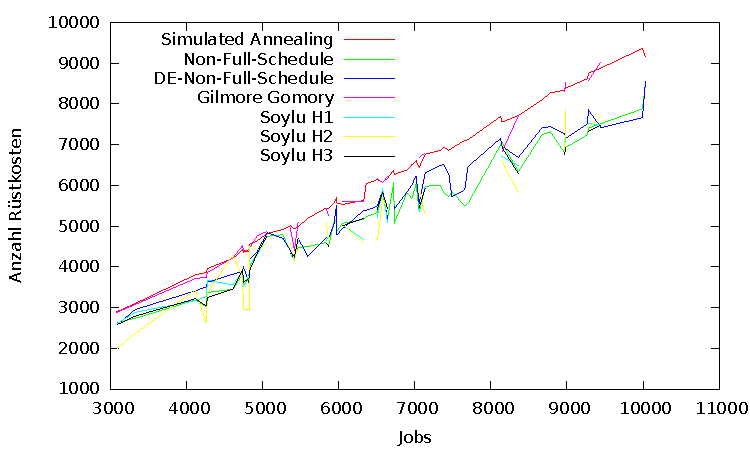
\includegraphics[width=.8\textwidth]{../prog/heuristics/plots/kbcoplot.pdf}
    \end{center}
    \caption{
        \label{abb:kbcoplot}
        Summer der Rüstkosten, die auftreten, nachdem $\pi$ mit der jeweiligen Heuristik erzeugt und anschließend ggf. korrigiert wurde.
        Jeder Ressourcenwechsel verursacht Rüstkosten in Höhe von $5$ Minuten.
    }
\end{figure}
Es ist zu sehen, dass gerade die Verfahren, die normalerweise sehr gute Ergebnisse liefern (z.B. Gilmore Gomory\footnote{
Wegen der zwei benachbarten dominierenden Maschinen ist die Gilmore-Gomory-Heuristik hier ein exaktes Verfahren.} oder Simulated Annealing)
hier besonders schlecht abschneiden, während $H_2$ hier (nach der Korrektur) vergleichsweise gute Resultate liefert.
Besonders auffällig ist, dass offenbar (bei allen Heuristiken) in fast jedem Zyklus die Ressource gewechselt werden muss.
Bei einer Instanzgröße von beispielsweise $n\approx 3000$ treten selbst bei dem dort besten Ergebnis ($H_2$) ca. 2000 Ressoucenwechsel auf.
Es fällt weiter auf, dass die Summe der Rüstkosten immer sehr viel größer ist als die zugehörige Summe der Zykluszeiten.

\subsubsection{Resultate des zweiten Dekompositionsansatzes}
\label{subsubsec:ResultateDKA2}
Beim zweiten Dekompositionsansatz muss zunächst die Zuordnung der Jobgruppen zu den Bins erfolgen.
Unmittelbar danach steht fest, wie oft eine Ressource gewechselt werden muss. 
Für den Fall, dass keine Jobgruppe geteilt wird, sind es genau $\tilde{n}-m$ Ressourcenwechsel, wenn eine Jobgruppe geteilt wird, sind es $\tilde{n}-m+1$, usw.
Da maximal $m-1$ Jobgruppen geteilt werden, können höchstens $\tilde{n}-1$ Ressourcenwechsel auftreten, was sehr viel weniger ist als beim ersten Dekompositionsansatz.
Die Laufzeiten des Binpackings für diese Instanzen betrugen jeweils unter 100 Millisekunden.
Die Summe der Rüstkosten ist in Abhängigkeit von $n$ in Abbildung \ref{abb:kbplotsetupsn} abgebildet.
\begin{figure}
    \begin{center}
        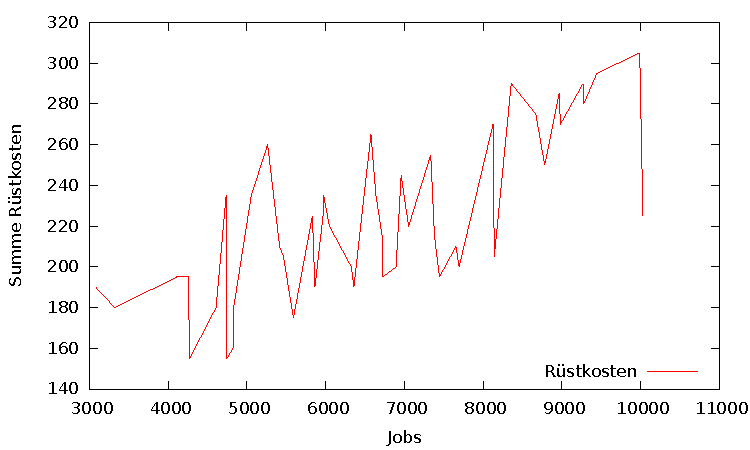
\includegraphics[width=.8\textwidth]{../prog/binpacking/results/kbplotsetupsn.pdf}
    \end{center}
    \caption{
        \label{abb:kbplotsetupsn}
        Summe der Rüstkosten.
    }
\end{figure}
Durchschnittlich mussten $1{,}113$ Jobgruppen geteilt werden und nur bei einer Instanz mussten $3$ Jobgruppen geteilt werden.

In Abbildung \ref{abb:kbplotn} sind die Resultate (Summe der Zykluszeiten) der einzelnen Algorithmenvarianten (s. Abschnitt \ref{sec:Algorithmenvarianten}) aufgetragen
bezogen auf die Anzahl der Jobs $n$.
Außerdem ist mit LB eine untere Schranke angegeben, die wie in Unterabschnitt \ref{subsubsec:BestimmungEinerUnterenSchranke} beschrieben berechnet wurde.
Bis auf des Simulated Annealing bestehen alle Varianten aus zwei Stufen: 
In der ersten Stufe werden die Bins den Stationen zugewiesen und in der zweiten werden die Jobgruppen in den Bins angeordnet.
\begin{figure}
    \begin{center}
        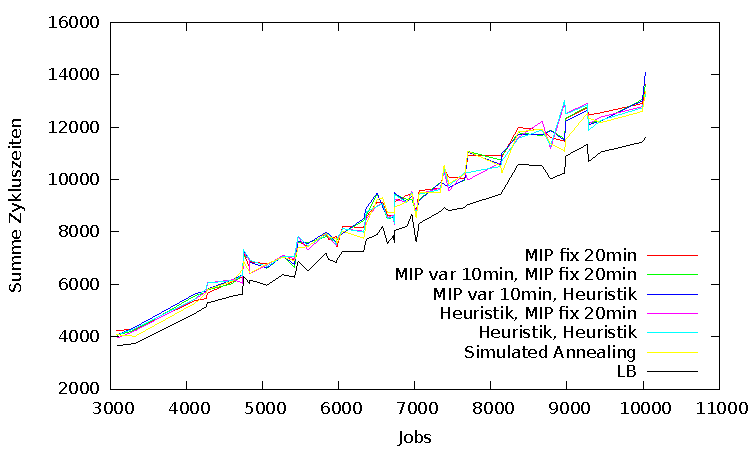
\includegraphics[width=.8\textwidth]{../prog/binpacking/results/kbplotn.pdf}
    \end{center}
    \caption{
        \label{abb:kbplotn}
        Summe der Zykluszeiten der einzelnen Algorithmenvarianten.
        Das MIP mit fixierten Bins (MIP fix) wurde in den jeweiligen Varianten 20 Minuten laufen gelassen
        und das mit freien Bins (MIP var) 10 Minuten.
    }
\end{figure}
Die Varianten liefern offenbar sehr ähnliche Ergebnisse, wobei keine Regelmäßigkeit zu erkennen ist, in welchen Situationen welche Variante am besten ist.
Es muss allerdings beachtet werden, dass einige Varianten dieses Ergebnis in sehr viel kürzerer Zeit erzielen als andere.
Die Laufzeit einer Algorithmenvariante wird im Wesentlichen durch die involvierten MIPs bestimmt.
Alle Verfahren, die nicht auf MIPs basieren terminierten jeweils in weniger als einer Sekunde.

In Abbildung \ref{abb:kbplotreln} sind dieselben Daten aufgetragen, allerdings als relative Differenz zur unteren Schranke.
\begin{figure}
    \begin{center}
        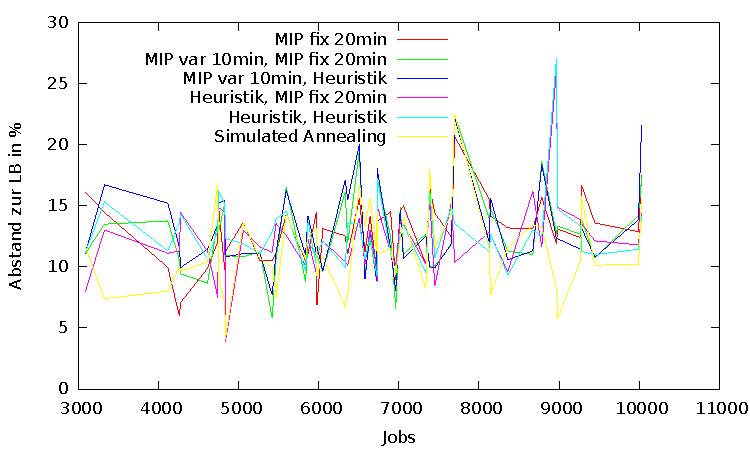
\includegraphics[width=.8\textwidth]{../prog/binpacking/results/kbplotreln.pdf}
    \end{center}
    \caption{
        \label{abb:kbplotreln}
        Unterschied zwischen den Algorithmenvarianten und der unteren Schranke (LB) in \%.
    }
\end{figure}
Dort ist zu erkennen, dass die untere Schranke und die Resultate der Algorithmenvarianten sich je nach Instanzgröße um ca. $5\%$ bis $25\%$ unterscheiden.
Wie zu erwarten war, ist dieser Abstand nicht optimal, aber auch nicht außerordentlich groß.
Es ist außerdem in Abbildung \ref{abb:kbplotreln} zu erkennen (besser als in \ref{abb:kbplotn}), dass in vielen Fällen Simulated Annealing die besten Resultate liefert.
Auch ist interessant, dass es einige wenige Fälle gibt, in denen das MIP mit fixierten Bins, also ohne vorherige Optimierung der Binreihenfolge, die beste Lösung liefert.
Das kann dadurch erklärt werden, dass per Zufall die initiale Binreihenfolge sehr gut sein kann und sogar besser als durch die Heuristik oder das MIP mit freien Bins 
(das in diesem Kontext auch eine Heuristik ist) ermittelte Reihenfolgen.

\begin{figure}
    \begin{center}
        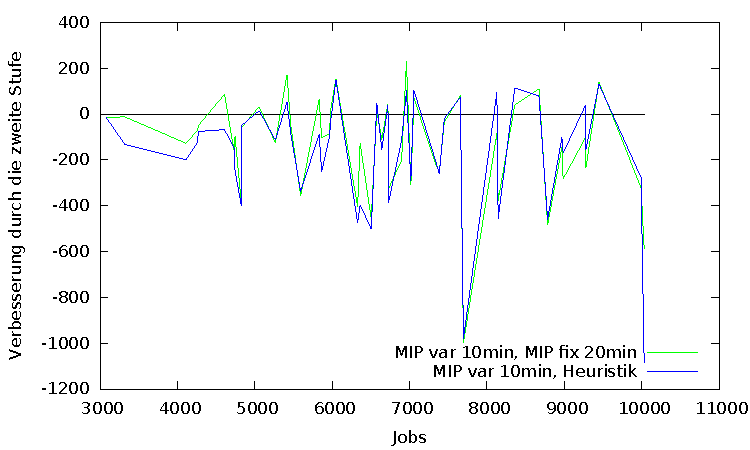
\includegraphics[width=.8\textwidth]{../prog/binpacking/results/kbplotmipdiffn.pdf}
    \end{center}
    \caption{
        \label{abb:kbplotmipdiffn}
        Vergleich der Algorithmenvarianten mit dem MIP mit freien Bins in erster Stufe.
    }
\end{figure}
Die beiden Algorithmenvarianten mit dem MIP mit freien Bins in der ersten Stufe benutzen dies jeweils nur, um eine Binreihenfolge zu generieren.
Die bis dahin gefundene beste Lösung des MIPs wird verworfen.
Es kommt daher vor, dass diese verworfene Lösung besser ist als die anschließend von der jeweils zweiten Stufe gefundene.
In Abbildung \ref{abb:kbplotmipdiffn} ist zu sehen, um wie viel das MIP mit fixierten Bins und die Heuristik 
eine durch das MIP mit freien Bins berechnete Lösung noch verbessern.
Negative Werte bedeuten, dass die zweite Stufe nicht in der Lage war, den Stand des MIPs mit freien Bins basierend auf dessen Binreihenfolge wieder zu erreichen.
Wie zu sehen ist, sind negative Werte häufiger als positive, was nicht erwartet wurde, 
da Tests dieser Algorithmenvarianten vielversprechend schienen.
Außerdem ist zu sehen, dass die Heuristik mit einer Laufzeit von unter einer Sekunde nur unwesentlich schlechtere und teilweise sogar bessere Ergebnisse liefert als 
das MIP mit fixierten Bins in 20 Minuten.

\subsubsection{Vergleich}
In Abbildung \ref{abb:kbcmaxplot} ist die Summe aus Zykluszeiten und Rüstkosten, also $C_{\max}$, des ersten Dekompositionsansatzes aufgetragen.
Da die Summe der Rüstkosten die der Zykluszeiten klar dominiert, weisen diese Kurven eine hohe Ähnlichkeit zu denen aus Abbildung \ref{abb:kbcoplot} auf,
sie sind im Wesentlichen lediglich nach oben verschoben.
\begin{figure}
    \begin{center}
        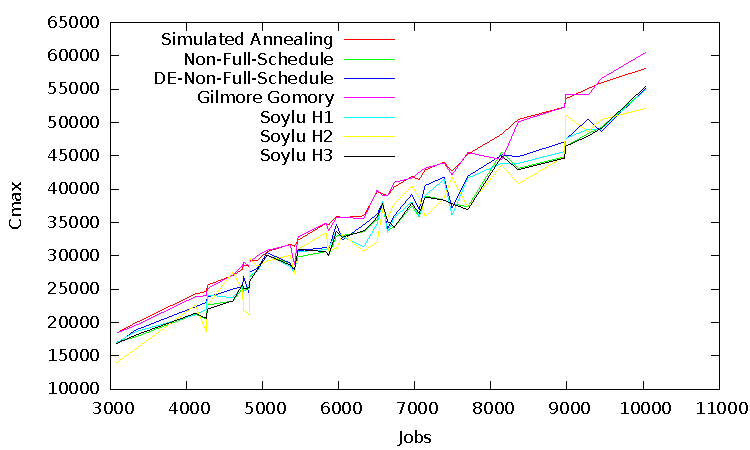
\includegraphics[width=.8\textwidth]{../prog/heuristics/plots/kbcmaxplot.pdf}
    \end{center}
    \caption{
        \label{abb:kbcmaxplot}
        Gesamtresultate der einzelnen Heuristiken im ersten Dekompositionsansatz.
    }
\end{figure}

In Abbildung \ref{abb:kbplotcmaxn} ist $C_{\max}$ für den zweiten Dekompositionsansatz aufgetragen.
Da die Rüstkosten verglichen mit den Zykluszeiten minimal sind, sehen die Abbildungen \ref{abb:kbplotcmaxn} und \ref{abb:kbplotn} sehr ähnlich aus.
\begin{figure}
    \begin{center}
        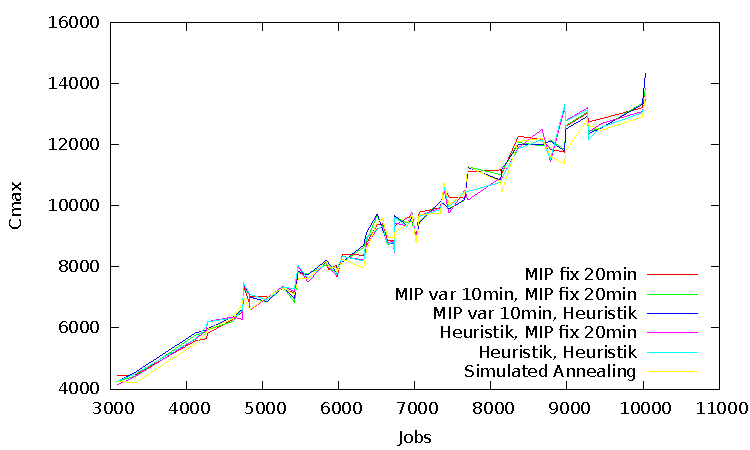
\includegraphics[width=.8\textwidth]{../prog/binpacking/results/kbplotcmaxn.pdf}
    \end{center}
    \caption{
        \label{abb:kbplotcmaxn}
        Gesamtresultate der einzelnen Algorithmenvarianten im zweiten Dekompositionsansatz.
    }
\end{figure}

Der Unterschied zwischen beiden Dekompositionsansätzen ist enorm.
Die Ansätze unterscheiden sich in etwa um den Faktor $4$.
Dieser große Unterschied war allerdings zu erwarten, da bei diesen Instanzen die Rüstkosten mit $s=5$ die Prozesszeiten mit $p_{ij}\in [0,2]$ dominieren.
Bei $s\approx 0{,}12$ würden beide Ansätze ähnliche Resultate liefern.


\subsection{Generierte Instanzen}
\label{subsec:GenerierteInstanzen}
Zusätzlich zu den Datensätzen des Küchenherstellers wurden zufällige Instanzen generiert, die im folgenden bezüglich der beiden Dekompositionsansätze evaluiert werden.
Diese Testreihe besteht aus 30 Instanzen mit $\tilde{n}=10,11,\ldots,40$ Jobgruppen.
Die Größen der Jobgruppen wurden jeweils gleichverteilt aus dem Intervall $[1,5\tilde{n}]$ gewählt und die Anzahl der zulässigen Ressourcen aus $[1,10]$.
Die Prozesszeiten auf den beiden dominierenden Maschinen liegen gleichverteilt zwischen $0{,}5$ und $2$.
Da jeder Wert für $\tilde{n}$ nur einmal vorkommt, wird auf den horizontalen Achsen der hier präsentierten Diagramme die Anzahl der Jobgruppen aufgetragen
statt wie in Unterabschnitt \ref{subsec:RealeInstanzen} die Anzahl der Jobs.

\subsubsection{Resultate des ersten Dekompositionsansatzes}
Die Resultate der Heuristiken, die eine initiale Jobreihenfolge $\pi$ generieren, sind in Abbildung \ref{abb:heurplot} dargestellt.
\begin{figure}
    \begin{center}
        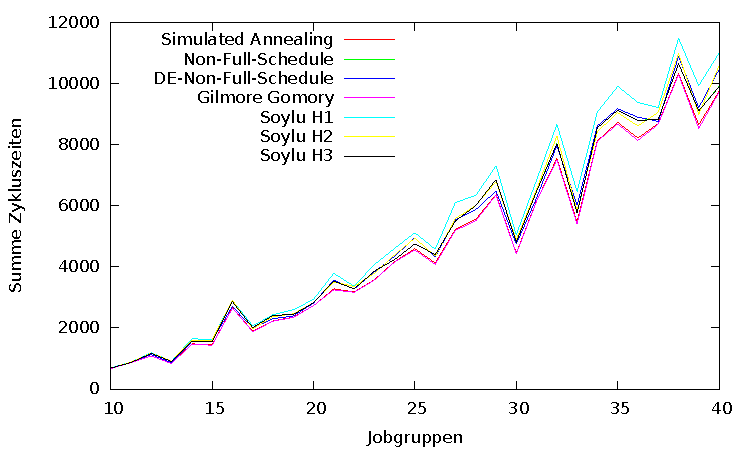
\includegraphics[width=.8\textwidth]{../prog/heuristics/plots/heurplot.pdf}
    \end{center}
    \caption{
        \label{abb:heurplot}
        Resultate der einzelnen Heuristiken vor der Korrektur.
    }
\end{figure}
Wie zu erwarten war, ist die Gilmore-Gomory-Heuristik (die hier optimale Ergebnisse liefert) am besten, Simulated Annealing am zweitbesten und $H_1$ am schlechtesten.
Allerdings sind die Unterschiede etwas geringer als bei den realen Instanzen (vgl. Abbildung \ref{abb:kbheurplot}).

In Abbildung \ref{abb:plot} sind die Resultate nach der Korrektur dargestellt.
\begin{figure}
    \begin{center}
        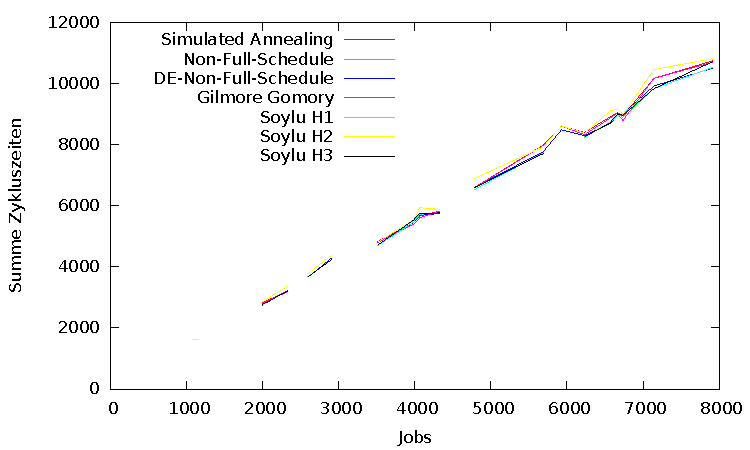
\includegraphics[width=.8\textwidth]{../prog/heuristics/plots/plot.pdf}
    \end{center}
    \caption{
        \label{abb:plot}
        Resultate der einzelnen Heuristiken nach der Korrektur.
    }
\end{figure}
Es fällt sofort auf, dass bei sehr vielen Instanzen keine zulässige Ressourcenzuweisung gefunden werden konnte (zu erkennen an den Lücken in den Graphen).
Während bei den realen Instanzen (vgl. Abbildung \ref{abb:kbplot}) aber immer mindestens eine Heuristik eine Reihenfolge generiert hat, 
für die eine zulässige Ressourcenzuweisung gefunden werden konnte, gibt es hier einige Instanzen, bei denen dies keine Heuristik schafft.
%TODO Dass aber für all diese Instanzen eine zulässige Zuweisung existiert, beweisen die Resultate des zweiten Dekompositionsansatzes (vgl. Abbildung \ref{abb:...}
Davon abgesehen sind die Lösungen wieder sehr ähnlich.
Die Differenz zwischen den Resultaten nach und vor der Korrektur sind in Abbildung \ref{abb:diffplot} zu sehen.
\begin{figure}
    \begin{center}
        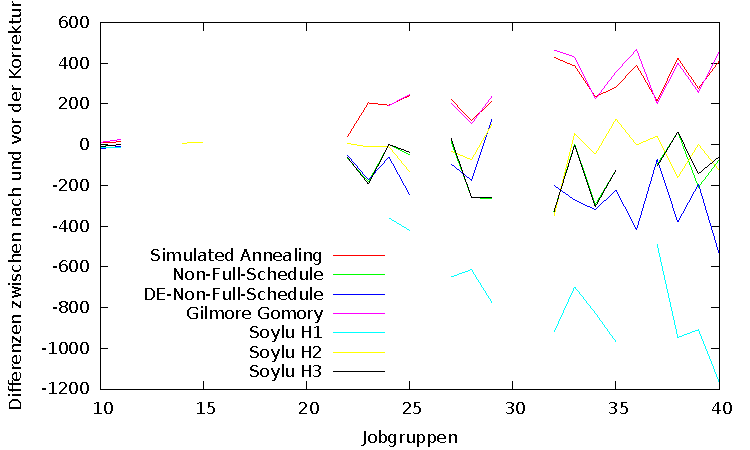
\includegraphics[width=.8\textwidth]{../prog/heuristics/plots/diffplot.pdf}
    \end{center}
    \caption{
        \label{abb:diffplot}
        Differenz zwischen den Resultaten nach und vor der Korrektur.
    }
\end{figure}
Auch bei diesen Instanzen wird die Lösung einiger Heuristiken durch die Korrektur sogar noch verbessert.
Die Rüstkosten, die nach der Korrektur der jeweiligen Heuristik verursacht werden, sind in Abbildung \ref{abb:coplot} dargestellt.
Da die Rüstkosten $s$ nicht vorgegeben sind, sind dort nur die Anzahl der Ressourcenwechsel und nicht die Höhe der Rüstkosten selbst zu sehen.
Außerdem ist in diesem Fall auf der horizontalen Achse die Anzahl der Jobs und nicht der Jobgruppen aufgetragen, 
da diese eine bessere Relation zu den Ressourcenwechseln bietet.
\begin{figure}
    \begin{center}
        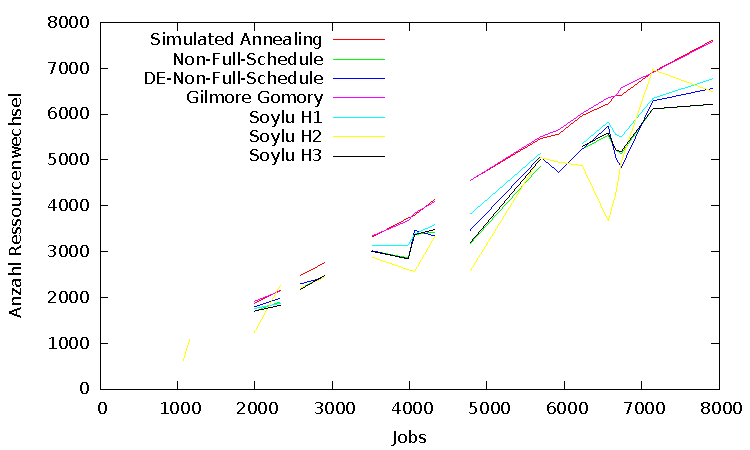
\includegraphics[width=.8\textwidth]{../prog/heuristics/plots/coplot.pdf}
    \end{center}
    \caption{
        \label{abb:coplot}
        Anzahl der Umrüstvorgänge, die auftreten, wenn $\pi$ mit der jeweiligen Heuristik erzeugt und anschließend korrigiert wurde.
    }
\end{figure}
%TODO siehe Vergleich
Wie zu sehen ist, sind wieder sehr viele Ressourcenwechseln notwendig.
Die Heuristiken, die ursprünglich die besten Ergebnisse lieferten (Gilmore Gomory und Simulated Annealing), schneiden hier deutlich am schlechtesten ab.
Ihre Kurven verlaufen nahezu linear und es muss offenbar fast in jedem Zyklus die Ressource gewechselt werden.
Relativ wenige Ressourcenwechsel werden offenbar durch die Resultate von $H_2$ verursacht.

\subsubsection{Resultate des zweiten Dekompositionsansatzes}
Bei den generierten Instanzen müssen beim Binpacking durchschnittlich $1{,}27$ Gruppen geteilt werden.
Dabei kommen Instanzen mit vielen Jobgruppen häufig ohne Teilung aus, während kleinere Instanzen bis zu $6$ Teilungen benötigen,
wie in Abbildung \ref{abb:plotsplits} zu sehen ist.
\begin{figure}
    \begin{center}
        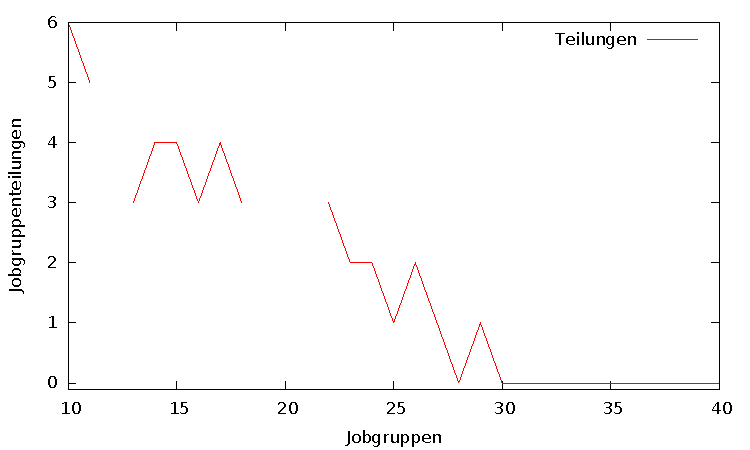
\includegraphics[width=.8\textwidth]{../prog/binpacking/results/plotsplits.pdf}
    \end{center}
    \caption{
        \label{abb:plotsplits}
        Anzahl der benötigten Jobgruppenteilungen.
    }
\end{figure}
Dort ist außerdem zu sehen, dass bei einigen Instanzen keine Lösung gefunden werden konnte.
Es war dort also nicht möglich, die Jobgruppen so anzuordnen, dass nur solche mit mehr als zwei Ressourcen geteilt werden.
Die Möglichkeit, mit zusätzlichen Bedingungen in der zweiten Stufe dafür zu sorgen, 
dass zwei Teilgruppen einer geteilten Jobgruppe mit nur einer Ressource sich nicht überlappen, wurde hier nicht weiter verfolgt.

In Abbildung \ref{abb:plot2} werden die Resultate der Algorithmenvarianten präsentiert.
\begin{figure}
    \begin{center}
        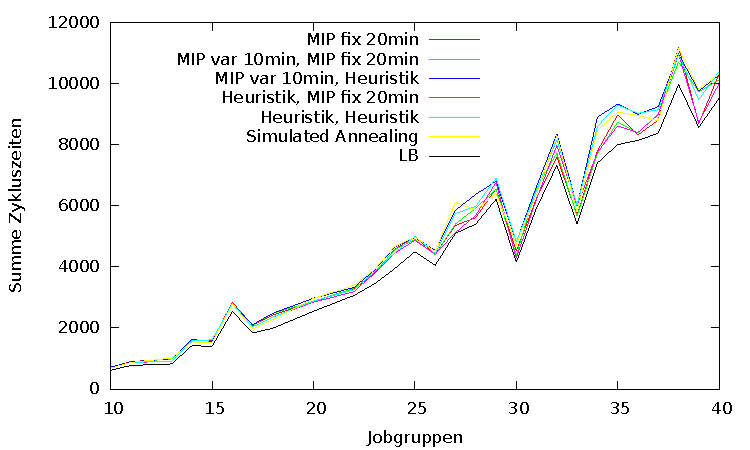
\includegraphics[width=.8\textwidth]{../prog/binpacking/results/plot.pdf}
    \end{center}
    \caption{
        \label{abb:plot2}
        Summe der Zykluszeiten der einzelnen Algorithmenvarianten. 
        Das MIP mit fixierten Bins (MIP fix) wurde in den jeweiligen Varianten 20 Minuten laufen gelassen und das mit freien Bins (MIP var) 10 Minuten.
    }
\end{figure}
Es lässt sich erkennen, dass die Varianten mit der Heuristik in der zweiten Stufe oft etwas schlechtere Ergebnisse liefern als die Varianten mit dem MIP mit fixierten Bins.
Außerdem kommen die Resultate aller Varianten dichter an die unteren Schranke heran als bei den realen Instanzen,
was durch einen Vergleich der Abbildungen \ref{abb:kbplotreln} und \ref{abb:plotrel} deutlich wird.
\begin{figure}
    \begin{center}
        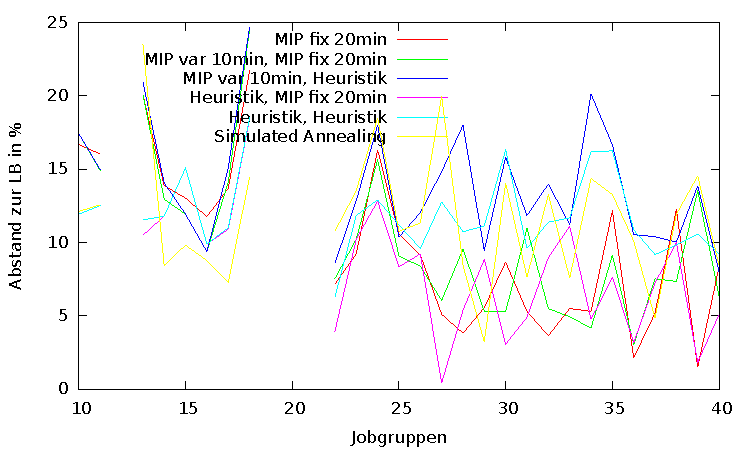
\includegraphics[width=.8\textwidth]{../prog/binpacking/results/plotrel.pdf}
    \end{center}
    \caption{
        \label{abb:plotrel}
        Relativer Abstand der Algorithmenvarianten zur unteren Schranke (LB).
    }
\end{figure}

In Abbildung \ref{abb:plotmipdiff} ist zu sehen, um wie viel die Heuristik und das MIP mit fixierten Bins das Resultat des MIPs mit variablen Bins verbessern konnten.
\begin{figure}
    \begin{center}
        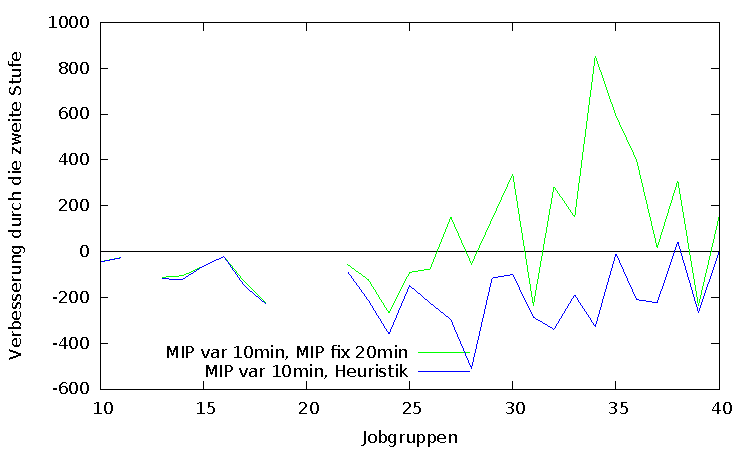
\includegraphics[width=.8\textwidth]{../prog/binpacking/results/plotmipdiff.pdf}
    \end{center}
    \caption{
        \label{abb:plotmipdiff}
        Vergleich der Algorithmenvarianten mit dem MIP mit freien Bins in erster Stufe.
    }
\end{figure}
Die Heuristik war offenbar nie in der Lage, auf Grundlage der vom MIP mit freien Bins generierten Binreihenfolge die Lösung dieses MIPs wieder zu erreichen.
Das MIP mit fixierten Bins hingegen konnte vor allem bei großen Instanzen diesen Wert teils deutlich verbessern.
Das kann dadurch erklärt werden, dass das MIP mit freien Bins bei kleinen Instanzen noch in der Lage ist, in relativ kurzer Zeit gute Lösungen zu erarbeiten.
Bei großen Instanzen hingegen kann das MIP mit fixierten Bins oft noch weit bessere Lösungen (basierend auf derselben Binreihenfolge) erzeugen.

\subsubsection{Vergleich}
Zum Vergleich sind in Abbildung \ref{abb:plotcomp} die Summen der Zykluszeiten zweier Repräsentanten je eines der beiden Dekompositionsansätze nebeneinander aufgetragen.
Für den ersten Dekompositionsansatz wurde $H_2$ gewählt, da dort die Anzahl der Ressourcenwechsel meist am niedrigsten war.
Für den zweiten Dekompositionsansatz fiel die Wahl auf die Algorithmenvariante mit der Heuristik in der ersten Stufe und dem MIP mit fixierten Bins in der zweiten.
Wie dort zu sehen ist, ist selbst bei $s=0$ der zweite Dekompositionsansatz fast bei allen Instanzen besser als der erste, wenn auch nur sehr gering.
\begin{figure}
    \begin{center}
        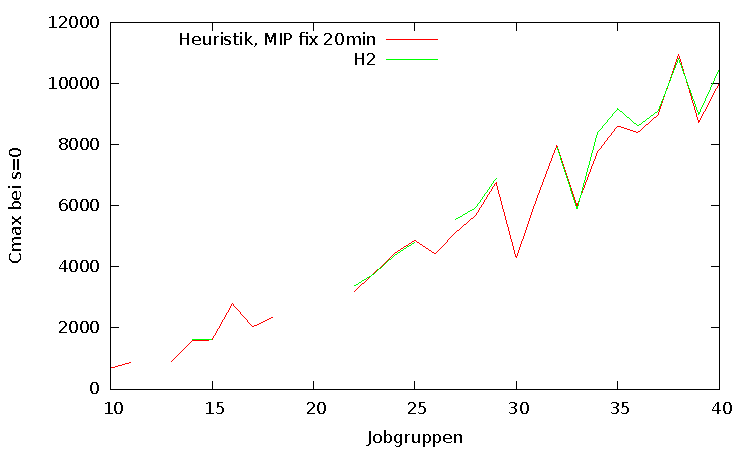
\includegraphics[width=.8\textwidth]{../prog/binpacking/results/plotcomp.pdf}
    \end{center}
    \caption{
        \label{abb:plotcomp}
        Direkter Vergleich von $C_{\max}$ zwischen zwei Vertretern der beiden Dekompositionsansätze bei $s=0$.
    }
\end{figure}
\begin{figure}
    \begin{center}
        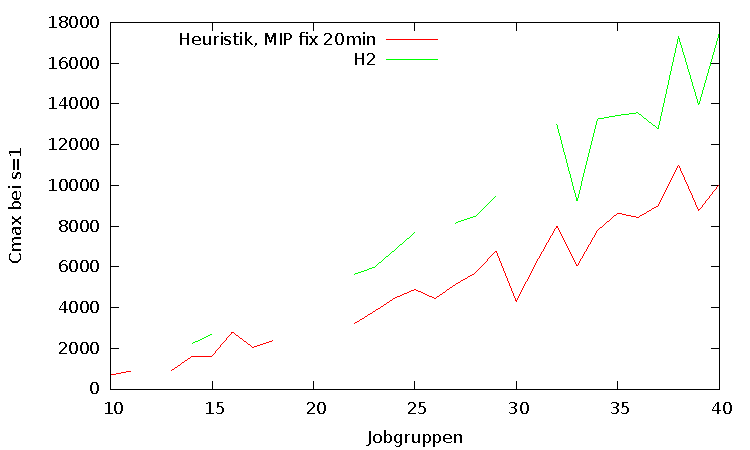
\includegraphics[width=.8\textwidth]{../prog/binpacking/results/plotcomp2.pdf}
    \end{center}
    \caption{
        \label{abb:plotcomp2}
        Direkter Vergleich von $C_{\max}$ zwischen zwei Vertretern der beiden Dekompositionsansätze bei $s=1$.
    }
\end{figure}
Ist $s=1$ (s. Abbildung \ref{abb:plotcomp2}), wird der Unterschied deutlich größer.

Es sollte daher bei Instanzen, die diesen generierten ähneln, der zweite Dekompositionsansatz gewählt werden.
Bei den realen Instanzen in Unterabschnitt \ref{subsec:RealeInstanzen} wäre der erste Dekompositionsansatz wenigstens für sehr 
geringe Rüstkosten im Vorteil gewesen.

\chapter{Fazit und Ausblick}
Die beiden Dekompositionsansätze liefern die erwarteten Ergebnisse:
Der erste eignet sich gut, wenn die Rüstkosten sehr viel kleiner sind als die Prozesszeiten und wenn viele Ressourcen vorhanden sind.
Bei seinen Lösungen muss regelmäßig die Ressource gewechselt werden.
Der Fall, dass eine Ressource wiederverwendet werden kann, bildet die Ausnahme.
Der zweite Dekompositionsansatz kommt hingegen mit einer minimalen Anzahl an Ressourcenwechseln aus und benötigt entsprechend wenige Ressourcen.
In der Praxis genügt es, wenn für die meisten Jobgruppen (die nicht größer als $\frac{n}{m}$ sind) nur eine Ressource 
und für einige wenige Jobgruppen noch eine zweite vorhanden ist für den Fall, dass Jobgruppen getrennt werden müssen.
Erstaunlich beim ersten Dekompositionsansatz ist, dass die Wahl der Methode zur Berechnung einer initialen Reihenfolge nahezu keine Rolle spielt,
obwohl die getesteten Heuristiken teilweise sehr unterschiedliche Ergebnisse produzieren.
Die Qualität der Lösung ist erst nach der Korrektur der initial erzeugten Reihenfolge absehbar.
Auch beim zweiten Dekompositionsansatz lässt sich nicht eindeutig sagen, welche Variante die beste ist.
Es lässt sich lediglich festhalten, dass Simulated Annealing, welches als einziges der vorgestellten Verfahren auf eine zeitliche Trennung der beiden Schritte
"`Anordnung der Bins"' und "`Anordnung der Jobgruppen in den Bins"' verzichtet, oft die besten Lösungen liefert und darüber hinaus eine weit bessere Laufzeit hat als die
Verfahren, in denen ein MIP involviert ist.

Da sowohl im zweiten Dekompositionsansatz als auch bei der Berechnung einer Jobreihenfolge ohne Ressourcen und Rüstkosten
die Simulated-Annealing-Ansätze sehr gute Lösungen liefern, wäre es interessant, 
weitere Verfahren zu entwickeln und zu verfeinern, die auf einer Nachbarschaftssuche basieren.
Gerade für den zweiten Dekompositionsansatz, der dem ersten zwar häufig überlegen scheint, 
aber in dieser Arbeit fast ausschließlich (bis auf Simulated Annealing) für den Spezialfall mit zwei dominierenden Maschinen, 
konstanten Rüstkosten und disjunkten Ressourcenmengen erarbeitet wurde,
ist ein Ansatz von Interesse, der diesen Restriktionen nicht unterliegt.
Auch scheint es vielversprechend, für beide Dekompositionsansätze die jeweiligen Heuristiken in CPLEX zu integrieren, 
damit beim Lösen der MIPs schneller besseren Schranken gefunden werden.
Da generell Heuristiken gute Lösungen in beiden Dekompositionsansätzen liefern, könnte auch über gänzlich andere Ansätze als den der Dekomposition nachgedacht werden,
etwa Heuristiken, die das gesamte Problem auf einmal lösen.

\newpage
\bibliographystyle{alphadin}
\bibliography{quellen}

\chapter*{Erklärung}
\noindent
Ich erkläre eidesstattlich, dass ich die vorliegende Arbeit selbstständig und ohne fremde Hilfe verfasst, 
andere als die angegebenen Quellen nicht benutzt und die den benutzten Quellen entnommenen Stellen als 
solche gekennzeichnet habe. Die Arbeit wurde bisher in gleicher oder ähnlicher Form keiner anderen 
Prüfungsbehörde vorgelegt.
\par
\vspace{10mm}
\noindent
Osnabrück, den 26. September 2014
\par
\vspace{12mm}
\noindent
Sebastian Brockmeyer

\end{document}
